\documentclass[12pt,a4paper,oneside]{book}
\usepackage[utf8]{vietnam}
\usepackage{amsmath}
\usepackage{graphicx}
\usepackage{algorithm2e}
\usepackage{fancyhdr}
\usepackage{algorithm2e}
\usepackage{mathtools}
\usepackage{tikz}
\usetikzlibrary{matrix}
\usepackage{nicematrix}
\usepackage{siunitx}
\usepackage{pgfplots}
\usepackage{graphicx}
\usepackage{multirow}
\usepackage[table,xcdraw]{xcolor}
\usepackage{bkthesis}

\addbibresource{refs.bib}

\title{Báo cáo thực tập ngoài trường} %Title of your type of project/Thesis (For example, Project 1, Milestone, Capstone...
\subtitle{FPGA Implementation of LDPC Decoder Architecture for Wireless Communication Standards} %Title of your type of project/Thesis
\csSupervise{ThS. Nguyễn Trung Hiếu} %Your supervise ofc
\cstuname{Vũ Nhật Huy} %Your name
\cstuid{2311267} %Your stu/id

\cttime{\today} %Date
\cttimeSpacing{5.25cm}

\thesislayout

\begin{document}

\coverpage

\frontmatter

\pagestyle{fancy}

% \begin{acknowledgments}
% Write the Acknowledgment here.
% \end{acknowledgments}

\newpage
\begin{abstract}
\textit{Em xin gửi lời cảm ơn chân thành và sự tri ân sâu sắc đối với thầy Nguyễn Trung Hiếu, giảng viên Bộ môn Điện tử trường Đại học Bách khoa - Đại học Quốc gia Thành phố Hồ Chí Minh, đã tạo điều kiện cho em có nhiều thời gian cho Báo cáo thực tập ngoài trường này. Và đồng thời em cũng xin chân thành cảm ơn thầy đã nhiệt tình hướng dẫn hướng dẫn giúp em hoàn thành tốt báo cáo này.}

\textit{Trong quá trình học tập, cũng như là trong quá trình làm bài báo cáo, do điều kiện khó khăn khó tránh khỏi sai sót, rất mong Thầy có thể thông cảm. Đồng thời do trình độ lý luận cũng như kinh nghiệm thực tiễn còn hạn chế nên bài báo cáo không thể tránh khỏi những thiếu sót, em rất mong nhận được ý kiến đóng góp từ Thầy để em học thêm được nhiều kinh nghiệm và sẽ hoàn thành tốt những Đồ án, Luận văn tốt nghiệp trong tương lai.}

\textit{EM xin chân thành cảm ơn Thầy!}

\textit{Chúc Thầy nhiều sức khỏe.}

\end{abstract}

\tableofcontents
%%\listofsymbols
%\newpage
\listoffigures
%\newpage
\listoftables

\mainmatter

%%%%%%%%%%%%%%%%%%%%

\chapter{Giới thiệu}
\section{Động lực nghiên cứu}
Mã kiểm tra chẵn lẻ mật độ thấp (Low-Density Parity-Check - LDPC) đóng vai trò quan trọng trong các hệ thống thông tin hiện đại nhờ khả năng sửa lỗi tối ưu. Cụ thể, các nghiên cứu \cite{1} đã chỉ rằng các mã LDPC bất thường nếu được thiết kế tối ưu có thể đạt ngưỡng hiệu suất chỉ cách giới hạn Shannon một khoảng cực kỳ nhỏ là $0.0045\text{ dB}$ ở tỷ lệ lỗi bit $\text{BER} = 10^{-6}$. Thậm chí, trong các mô phỏng thực tế với chiều dài khối lên tới $10^7$ thì các bộ giải mã này vẫn duy trì khả năng hoạt động cực kỳ ổn định và đạt mức cách giới hạn Shannon chỉ $0.04\text{ dB}$ ở mức $\text{BER} = 10^{-6}$. Nhờ đặc tính vượt trội này mà mã LDPC đã trở thành một phần không thể thiếu trong các chuẩn truyền thông không dây băng thông rộng phổ biến như IEEE 802.11n/ad/ay/ax (Wifi), IEEE 802.16e (WiMAX) và mạng di động thế hệ mới ETSI 5G.

Trong thực tế triển khai, các ứng dụng truyền thông hiện đại đòi hỏi tốc độ dữ liệu ngày càng cao và khả năng tương thích linh hoạt với nhiều tiêu chuẩn khác nhau. Tuy nhiên, phần lớn các kiến trúc giải mã song song hiện nay chỉ được thiết kế cố định cho một tiêu chuẩn truyền thông duy nhất hoặc một chiều dài từ mã cụ thể, dẫn đến sự thiếu linh hoạt. Bên cạnh đó, các nghiên cứu trước đây \cite{2}, \cite{3}, \cite{4} thường lạm dụng tài nguyên bộ nhớ khối (BRAM) để lưu trữ các giá trị nội bộ mà chưa chú trọng đến việc tối ưu hóa cách thức lưu trữ ma trận kiểm tra chẵn lẻ thưa (Sparse Parity-Check Matrix), gây lãng phí tài nguyên phần cứng trên chip. Để giải quyết triệt để, kiến trúc bộ giải mã đề xuất chỉ lưu trữ ma trận kiểm tra chẵn lẻ cơ sở (base parity-check matrix) $H_b$. Khối dữ liệu này được nén thông qua 3 vector nội bộ: \textit{vals} (chứa các phần tử có giá trị khác -1), \textit{pos} (chứa chỉ số cột tương ứng) và \textit{elementSize} (chứa số lượng phần tử khác -1 trong mỗi hàng). Phương pháp này giúp giảm thiểu đột phá dung lượng BRAM cần thiết. 

Việc giải quyết bài toán tối ưu hóa tài nguyên lưu trữ đồng thời tăng cường khả năng cấu hình cho bộ giải mã là vô cùng cấp thiết. Một kiến trúc giải mã QC-LDPC có thể tái cấu hình linh hoạt sẽ giúp giảm thiểu chi phí thiết kế phần cứng và đẩy nhanh tốc độ xử lý. Kết quả của nghiên cứu này có thể ứng dụng trực tiếp vào các hệ thống hạ tầng viễn thông không dây tốc độ cao và các thiết bị lưu trữ thế hệ mới, đáp ứng đồng thời cả hai tiêu chuẩn phổ biến là WiMAX và WiFi trên cùng một nền tảng phần cứng.

\section{Tình hình nghiên cứu}
Trong kỷ nguyên truyền thông tốc độ cao, yêu cầu khắt khe về băng thông đã thúc đẩy vô số công trình nghiên cứu về kiến trúc giải mã LDPC song song được công bố trong thập kỷ qua. Dù các kiến trúc này đã chứng minh được hiệu năng xử lý ở các mức độ nhất định, chúng vẫn tồn tại những nhược điểm về kiến trúc lưu trữ và độ linh hoạt, cụ thể:  
\begin{itemize}
    \item Hạn chế về tính linh hoạt phần cứng. Tiêu biểu như nghiên cứu của C. Kun \cite{2}, kiến trúc giải mã được thiết kế cố định cho một khung tiêu chuẩn cụ thể. Điều này đồng nghĩa với việc khi hệ thống cần chuyển đổi từ giao thức WiFi sang WiMAX thì toàn bộ phần cứng phải được thiết kế và tổng hợp lại từ đầu, gây lãng phí thời gian và tốn kém chi phí triển khai.
    \item Ngoài ra trước đây có khá nhiều thiết kế đã áp dụng phương pháp lưu trữ dữ liệu tính toán nội bộ trực tiếp lên BRAM mà không nén dữ liệu. Nghiên cứu của S. Mhaske \cite{3} là một ví dụ minh họa rõ nét. Dù kiến trúc giải mã thuật toán này đạt được tốc độ băng thông lên tới $2.48 Gb/s$, nhưng lại tiêu tốn một lượng BRAM do không tối ưu hóa việc lưu trữ ma trận thưa. Việc lạm dụng BRAM theo cách truyền thống không chỉ gây lãng phí mà còn làm phức tạp hóa quá trình truy xuất dữ liệu song song, dễ tạo ra các điểm nghẽn băng thông khi mở rộng số lượng lõi giải mã.  
    \item Mặc dù đã có một số ít các công trình nghiên cứu bắt đầu chú ý đến việc tối ưu hóa bộ nhớ,như công trình của S. Nimara \cite{4} đề xuất một kiến trúc giải mã đa từ mã với hiệu suất sử dụng BRAM tốt hơn. Tuy nhiên thì công trình này vẫn thiếu đi khả năng tham số hóa để hỗ trợ đa chuẩn truyền thông băng thông rộng trên cùng một thiết kế nguyên khối. Ngoại trừ số ít nghiên cứu cung cấp được bộ giải mã linh hoạt nhưng phần lớn các kiến trúc hiện hành vẫn chưa giải quyết được bài toán cân bằng giữa tối ưu bộ nhớ và tính linh hoạt đa chuẩn.  
\end{itemize}

Chính từ những nhược điểm này thì việc phát triển một kiến trúc giải mã QC-LDPC kết hợp sử dụng thuật toán Min-Sum và có khả năng cấu hình bằng tham số là vô cùng cấp thiết. Kiến trúc đề xuất trong báo cáo này kỳ vọng giải quyết toàn diện các nhược điểm trên, đạt được băng thông giải mã lên tới $1.2 Gbps$ ở tần số hoạt động $240 MHz$ mà vẫn giữ mức tiêu thụ tài nguyên phần cứng cực kỳ tối ưu trên FPGA.

% Fig. \ref{fig:logoyrgb} illustrates an example Image in the report. The Image should have a caption, and the caption must be placed after the Image. The "label" for figures should begin with "fig:name" and the name should be related to the content of the figure.

% \begin{figure}[H]
%     \centering
%     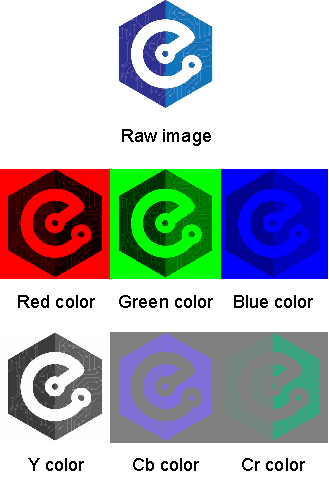
\includegraphics[width=.35\linewidth]{images/RGBtoYUV.pdf}  
%     \caption{The logo of the Department of Electronics in RGB and YCbCr color spaces}
%     \label{fig:logoyrgb}
% \end{figure}

% \section{Thesis Contributions}
% This section should outline the specific contributions of your thesis, such as:

% \begin{itemize}
%     \item New theories, models, or frameworks developed.
%     \item Novel methodologies or approaches proposed.
%     \item Significant findings or insights.
%     \item Practical implementations or applications.
% \end{itemize}

\section{Cấu trúc báo cáo}
Tổng quan toàn bộ quá trình thực hiện và triển khai bộ giải mã LDPC của bản báo cáo này được cấu trúc thành 7 chương như sau:
\begin{itemize}
    \item[] Chương 1: Giới thiệu.
    \item[] Chương 2: Cơ sở lý thuyết.
    \item[] Chương 3: Thiết kế và thực hiện phần mềm.
    \item[] Chương 4: Thiết kế và thực hiện phần cứng.
    \item[] Chương 5: Mô phỏng phần cứng.
    \item[] Chương 6: Kết quả thực hiện.
    \item[] Chương 7: Kết luận và hướng phát triển.
\end{itemize}
%%%%%%%%%%%%%%%%%%%%

\chapter{Cơ sở lý thuyết}
\section{Tổng quan về Mã Kiểm Tra Chẵn Lẻ Mật Độ Thấp (LDPC)}
LDPC là một lớp mã khối tuyến tính được phát triển ban đầu bởi Gallager vào năm 1963 \cite{5}. Đặc tính tuyến tính này cho phép mã được áp dụng trực tiếp lên các khối dữ liệu nguồn để thực hiện chức năng phát hiện và sửa lỗi trên kênh truyền nhiễu. Dù từng bị lãng quên trong nhiều thập kỷ do giới hạn phần cứng, mã LDPC đã trỗi dậy mạnh mẽ sau khi được MacKay và Neal khám phá lại vào cuối những năm 1990 \cite{6}.

Khái niệm mật độ thấp xuất phát từ đặc điểm cấu trúc hình học của ma trận kiểm tra chẵn lẻ $H$ (parity-check matrix) đại diện cho mã. Ma trận $H$ là một ma trận thưa, nghĩa là số lượng phần tử có giá trị bằng `1' chiếm tỷ lệ rất nhỏ so với số lượng phần tử mang giá trị bằng `0' bên trong ma trận. 

Một mã khối tuyến tính LDPC đều loại $(N, K)$ được biểu diễn cấu trúc thông qua ma trận kiểm tra $H$ có kích thước $M \times N$, với $M \ge N - K$ hàng và $N$ cột. Khi biểu diễn dưới dạng đồ thị hai phía Tanner, cấu trúc này bao gồm 2 thành phần chính sau:  
\begin{itemize}
    \item Các nút kiểm tra (Check Nodes - CN): Đại diện bởi $M$ hàng của ma trận $H$, đóng vai trò kiểm tra tính ràng buộc chẵn lẻ của các phương trình toán học.  
    \item Các nút biến (Variable Nodes - VN): Đại diện bởi $N$ cột của ma trận $H$, tương ứng trực tiếp với các phần tử bit cấu thành nên một từ mã. 
\end{itemize}

Trong các ứng dụng thực tế, các tiêu chuẩn truyền thông không dây băng thông rộng như WiFi và WiMAX không sử dụng mã LDPC mà sử dụng một biến thể gọi là mã LDPC tuần hoàn (QC-LDPC). Đây là nền tảng toán học cốt lõi cho phép triển khai kiến trúc giải mã song song trên phần cứng FPGA. Đặc tính tựa vòng thể hiện ở chỗ ma trận kiểm tra chẵn lẻ $H$ được cấu trúc từ nhiều ma trận con vuông. Các ma trận con này được tạo ra bằng cách dịch vòng một ma trận đơn vị theo các giá trị dịch chuyển xác định.

Nhờ tính chất này, quá trình triển khai phần cứng không cần phải lưu trữ toàn bộ ma trận $H$ khổng lồ. Thay vào đó, bộ giải mã chỉ cần lưu trữ ma trận kiểm tra chẵn lẻ cơ sở $H_b$ (base parity-check matrix). Việc biểu diễn $H_b$ giúp giảm thiểu đáng kể tài nguyên bộ nhớ BRAM cần thiết trên chip. Bên cạnh đó, kích thước của các ma trận con tựa vòng được ký hiệu là hệ số khai triển từ mã $z$ (codeword circulant size), quyết định trực tiếp đến mức độ song song hóa của bộ giải mã. Cụ thể, kiến trúc phần cứng có thể cập nhật đồng thời dữ liệu của $z$ nút biến, cho phép tăng tốc độ thông lượng lên gấp nhiều lần.

\section{Thuật Toán Giải Mã Min-Sum}
Thuật toán giải mã Min-Sum là một phiên bản đơn giản hóa của thuật toán Belief Propagation (BP). Sự đơn giản hóa này được thực hiện bằng cách giảm thiểu tối đa độ phức tạp tính toán tại các khối chức năng chịu trách nhiệm cập nhật nút kiểm tra (Check Node Update - CNU). So với thuật toán BP gốc, việc ứng dụng thuật toán Min-Sum giúp giảm thiểu đáng kể tài nguyên phần cứng tiêu thụ cũng như làm giảm độ phức tạp xử lý toán học của khối CNU \cite{7} mà vẫn duy trì được hiệu suất sửa lỗi ổn định.

Hệ thống giải mã quy ước các đại lượng toán học cơ bản bao gồm:
\begin{itemize}
    \item $c_n$: Biểu thị cho bit thứ $n$ của một từ mã phát đi từ nguồn.
    \item $y_n$: Giá trị tín hiệu thu được từ kênh truyền ở đầu vào bộ giải mã.
    \item $r_{mn}[k]$: Thông điệp truyền từ nút kiểm tra $m$ đến nút biến $n$ tại vòng lặp thứ $k$ (thông điệp Check-to-Variable - CTV).
    \item $q_{mn}[k]$: Thông điệp truyền từ nút biến $n$ đến nút kiểm tra $m$ tại vòng lặp thứ $k$ (thông điệp Variable-to-Check - VTC).
    \item $N(m)$: Tập hợp các nút biến tham gia vào phương trình kiểm tra của nút kiểm tra $m$.
    \item $M(n)$: Tập hợp các nút kiểm tra liên kết trực tiếp với nút biến $n$.
    \item $N(m) \setminus n$: Tập hợp các nút biến thuộc $N(m)$ ngoại trừ chính nút biến vị trí $n$.
    \item $M(n) \setminus m$: Tập hợp các nút kiểm tra thuộc $M(n)$ ngoại trừ chính nút kiểm tra vị trí $m$.
\end{itemize}
Thuật toán giải mã Min-Sum được vận hành tuần tự qua hai giai đoạn chính: 

\textbf{Bước 1: Khởi tạo (Initialization).} Tại bước này, giá trị xác suất kênh truyền $p_n$ (thông tin nội tại) của nút biến $n$ được xác định dựa trên tỷ số của xác suất tiên nghiệm:
\begin{equation}
    p_n = \log \frac{P(y_n | c_n = 0)}{P(y_n | c_n = 1)}
    \label{eq:1}
\end{equation}
Đồng thời, giá trị ban đầu của các thông điệp CTV được thiết lập bằng không: $r_{mn}[0] = 0$. 
  
\textbf{Bước 2: Giải mã lặp (Iterative Decoding).} Tại vòng lặp thứ $k$, thông điệp VTC là $q_{mn}[k]$ được tổng hợp bằng cách cộng thông tin nội tại của kênh với tổng các thông điệp phản hồi từ các nút kiểm tra liên kết còn lại thông qua công thức:
\begin{equation}
    q_{mn}[k] = p_n + \sum_{m' \in \{M(n) \setminus m\}} r_{m'n}[k-1]  
\end{equation}

Bộ giải mã tiến hành thực hiện phép quyết định cứng bằng cách tính toán giá trị xác suất hậu nghiệm (A-Posterior Probability - APP) $\Lambda_n[k]$ tại nút biến $n$ hiện tại:
\begin{equation}
    \Lambda_n[k] = p_n + \sum_{m' \in M(n)} r_{m'n}[k-1]
\end{equation}

Giá trị của bit kết quả $x_n$ thuộc vectơ từ mã ước lượng sẽ được xác định theo quy tắc:
\begin{equation}
    x_n = \begin{cases} 0 & \text{nếu } \Lambda_n[k] > 0 \\ 1 & \text{ngược lại} \end{cases}
    \label{eq:5}
\end{equation}

Vòng lặp giải mã sẽ kết thúc hoàn toàn khi vectơ kết quả $x = [x_1, x_2, \dots, x_N]$ thỏa mãn đồng thời tất cả các phương trình kiểm tra chẵn lẻ mang tính tuyến tính của ma trận:
\begin{equation}
    H \cdot x = 0
    \label{eq:6}
\end{equation}

Hoặc tiến trình lặp cũng sẽ tự động dừng lại nếu số vòng lặp hiện tại đạt đến giá trị ngưỡng tối đa được thiết lập từ trước trong cấu hình phần cứng hệ thống. Nếu từ mã hợp lệ, chế độ xuất kết quả được kích hoạt để đưa dữ liệu đã sửa lỗi ra ngoài đầu ra.  

Nếu phép toán kiểm tra ma trận không thỏa mãn ($H \cdot x \neq 0$), thông điệp kiểm tra phản hồi ngược lại $r_{mn}[k]$ gửi đến nút biến $m$ sẽ được tính toán dựa trên tích các dấu và giá trị cực tiểu của các thông điệp VTC thuộc tập liên kết loại trừ:
\begin{equation}
    r_{mn}[k] = \left( \prod_{n' \in \{N(m) \setminus n\}} sign(q_{mn'}[k]) \right) \times \left( \alpha \times \min_{n' \in \{N(m) \setminus n\}} \{|q_{mn'}[k]|\} \right)
\end{equation}

Trong đó, $\alpha$ là hệ số tỷ lệ điều chỉnh cố định ($\alpha \le 1$) nhằm bù đắp cho sự suy giảm biên độ do việc đơn giản hóa từ BP sang Min-Sum.
\subsection{Biểu thức rút gọn phục vụ tối ưu hóa phần cứng}
Để tối ưu hóa kiến trúc đọc/ghi song song dữ liệu từ bộ nhớ cổng kép (Dual-port BRAM) trên FPGA, cấu trúc toán học của thuật toán được tinh chỉnh lại. Các phép tính được đưa về quan hệ trực tiếp giữa giá trị APP tổng thể và các thông điệp cập nhật nhằm giảm độ trễ logic.  
\begin{itemize}
    \item Thay vì thực hiện phép cộng tích lũy, VTC được trích xuất trực tiếp bằng cách trừ thông điệp CTV của vòng trước khỏi APP hiện tại:
    \begin{equation}
        VTC_n=APP_n-CTV_n, \quad n=1...d_r
        \label{eq:2}
    \end{equation}
    với $d_r$ là trọng số hàng của ma trận kiểm tra.  
    \item Tính toán CTV mới:
    \begin{equation}
        CTV_{new\_n}=\prod_{k=1}^{N}\text{sign}(VTC_k)\times\text{sign}(VTC_n)\times\min(\vert{}VTC\vert{})
        \label{eq:3}
    \end{equation}
    Biểu thức này được hiện thực hóa bằng mạng so sánh logic kết hợp với các cổng logic XOR để xử lý dấu. 
    \item Cập nhật giá trị APP mới cho vòng lặp kế tiếp:
    \begin{equation}
        APP_{new\_n}=VTC_n+CTV_{new\_n}, \quad n=1...d_r
        \label{eq:4}
    \end{equation}
    Kết quả APP mới này sẽ được ghi đè trở lại BRAM, chuẩn bị cho chu kỳ giải mã tiếp theo.  
\end{itemize}
\subsection{Ví dụ tổng quát về thuật toán Min-Sum}
Giả sử ta có từ mã $c = [0\ 0\ 1\ 0\ 1\ 1],$ được truyền qua kênh truyền với xác suất lai chéo $p=0.2$ và giá trị tín hiệu thu được từ kênh truyền $y = [1\ 0\ 1\ 0\ 1\ 1]$. \cite{8}

Đầu tiên, ta tiến hành thiết lập ma trận kiểm tra chẵn lẻ $H$ với kích thước $4\times 6$ (4 phương trình kiểm tra và 6 bit từ mã) để tiện quan sát:
\begin{equation}
    H = \begin{bmatrix} 1 & 1 & 0 & 1 & 0 & 0 \\ 0 & 1 & 1 & 0 & 1 & 0 \\ 1 & 0 & 0 & 0 & 1 & 1 \\ 0 & 0 & 1 & 1 & 0 & 1\end{bmatrix}
\end{equation}

Từ \ref{eq:1} ta có giá trị xác suất kênh truyền như sau:
\begin{equation}
    p_n = \begin{cases} 
P(y_n|c_n=0)=\log \dfrac{p}{1-p}, & \text{nếu } y_i = 1, \\
P(y_n|c_n=1)=\log \dfrac{1-p}{p}, & \text{nếu } y_i = 0.
\end{cases}
\end{equation}
Như vậy đối với kênh truyền này ta lần lượt có giá trị như sau:
\begin{equation}
    P(y_n|c_n=0) = \log \frac{0.2}{1-0.2} = -1.3863,\ P(y_n|c_n=1) = \log \frac{1-0.2}{0.2} = 1.3863
\end{equation}
Từ đó ta có dãy Log-Likelihood Ratio (LLR) thu được từ kênh truyền như sau:
\begin{equation}
    p = [-1.3863, 1.3863, -1.3863, 1.3863, -1.3863, -1.3863]
\end{equation}

Tại vòng lặp 0, các thông điệp VTC chưa qua xử lý, nên sẽ nhận chính giá trị LLR ban đầu này:
\begin{itemize}
    \item[]$n = 1$: $VTC_{1,1} = -1.3863,\ VTC_{1,3} = -1.3863$
    \item[]$n = 2$: $VTC_{2,1} =\ \ 1.3863,\ VTC_{2,2} =\ \ 1.3863$
    \item[]$n = 3$: $VTC_{3,2} = -1.3863,\ VTC_{3,4} = -1.3863$
    \item[]$n = 4$: $VTC_{4,1} =\ \ 1.3863,\ VTC_{4,4} =\ \ 1.3863$
    \item[]$n = 5$: $VTC_{5,2} = -1.3863,\ VTC_{5,3} = -1.3863$
    \item[]$n = 6$: $VTC_{6,3} = -1.3863,\ VTC_{6,4}= -1.3863$
\end{itemize}

Tiếp đến, ta cập nhật giá trị CTV thông qua công thức \ref{eq:3} ứng với 3 nút kiểm tra:
\begin{itemize}
    \item[]$m = 1$: $CTV_{1,1} = 1.3863$, $CTV_{1,2} = -1.3863$, $CTV_{1,4} = -1.3863$
    \item[]$m = 2$: $CTV_{2,2} = 1.3863$, $CTV_{2,3} = -1.3863$, $CTV_{2,5} = -1.3863$
    \item[]$m = 3$: $CTV_{3,1} = 1.3863$, $CTV_{3,5} =\ \ 1.3863$, $CTV_{3,6} =\ \ 1.3863$
    \item[]$m = 4$: $CTV_{4,3} = -1.3863$, $CTV_{4,4} = 1.3863$, $CTV_{4,6} = -1.3863$
\end{itemize}

Tiếp theo, ta tiến hành cập nhật giá trị APP mới thông qua \ref{eq:4} cho vòng lặp tiếp theo:
\begin{itemize}
    \item[] $APP_1 = p_1 + CTV_{1,1} + CTV_{3,1} = -1.3863 + 1.3863 + 1.3863 = 1.3863$
    \item[] $APP_2 = p_2 + CTV_{1,2} + CTV_{2,2} = 1.3863 -1.3863 + 1.3863 = 1.3863$
    \item[] $APP_3 = p_3 + CTV_{2,3} + CTV_{4,3} = -1.3863 -1.3863 -1.3863= -4.1589$
    \item[] $APP_4 = p_4 + CTV_{1,4} + CTV_{4,4}= 1.3863 - 1.3863 + 1.3863= 1.3863$
    \item[] $APP_5 = p_5 + CTV_{2,5} + CTV_{3,5} = -1.3863 - 1.3863 + 1.3863 = -1.3863$
    \item[] $APP_6 = p_6 + CTV_{3,6} + CTV_{4,6}= -1.3863 + 1.3863 -1.3863= -1.3863$
\end{itemize}

Căn cứ vào dấu của bộ giá trị APP mới, hệ thống đưa ra phép quyết định cứng dựa vào quy tắc \ref{eq:5}. Khi ấy ta có từ mã dự đoán:
\begin{equation}
    x = [0\ 0\ 1\ 0\ 1\ 1]
\end{equation}
Để kiểm tra nếu từ mã $x$ đã đúng hay chưa, ta áp dụng \ref{eq:6} và thu được:
\begin{equation}
    \mathbf{x}H^T = [0 \quad 0 \quad 1 \quad 0 \quad 1 \quad 1] \begin{bmatrix} 1 & 0 & 1 & 0 \\ 1 & 1 & 0 & 0 \\ 0 & 1 & 0 & 1 \\ 1 & 0 & 0 & 1 \\ 0 & 1 & 1 & 0 \\ 0 & 0 & 1 & 1 \end{bmatrix} = [0 \quad 0 \quad 0 \quad 0]
\end{equation}
Như vậy $x$ là từ mã hợp lệ.
% This chapter should cover foundational concepts and background information necessary for understanding your research. Include:

% \begin{itemize}
%     \item Basic theories and principles.
%     \item Key terminology and definitions.
%     \item Relevant technologies and tools.
%     \item Any assumptions or limitations.
% \end{itemize}

% Anything you want to cite should be cited with the "cite{}" command. For example, This is a sentence from \cite{networkworld2023idc} (A Website) or this is a sentence from \cite{xu2022improving} (A paper). You can put the citing bib in the file "refs.bib", you can write the bib information yourself, get it from Google Scholar, or use Zotero (free) the best bib library software. The cite name is usually automatically generated, but you can change it to some name you remember, but don't number it. \cite{9493380}

% Table \ref{tab:example} is an example table in the report. The Table also needs a caption, and the caption must be placed before the Table. The "label" for table should begin with "tab:name" and the name should be related to the content of the table. You could try to ask ChatGPT combine data to a \LaTeX \ table for you or use \url{https://www.tablesgenerator.com}. Here' another basic table, Table \ref{tab:basic}.

% \begin{table}[H]
% \caption{JPEG specification defined compression process}\label{tab:example}
% \resizebox{\columnwidth}{!}{%
% \begin{tabular}{|
% >{\columncolor[HTML]{FFCCC9}}l |
% >{\columncolor[HTML]{EFEFEF}}l |}
% \hline
% \multicolumn{1}{|c|}{\cellcolor[HTML]{FFCCC9}\textbf{Baseline}}                                                                                                                                                                              & \multicolumn{1}{c|}{\cellcolor[HTML]{EFEFEF}\textbf{Lossless}}                                                                                                                                   \\ \hline
% \begin{tabular}[c]{@{}l@{}}- DCT-based process\\ - 8-bit samples\\ - Sequential\\ - Huffman coding with up to 2 \\ AC tables and 2 DC tables\\ - Up to 4 components\end{tabular}                                                                & \begin{tabular}[c]{@{}l@{}}- Predictive process\\ - Between 2-bit and 16-bit samples\\ - Huffman or Arithmetic coding with up to \\4 AC tables and 4 DC tables\\ - Up to 4 components\end{tabular} \\ \hline
% \multicolumn{1}{|c|}{\cellcolor[HTML]{EFEFEF}\textbf{Extended DCT based}}                                                                                                                                                                    & \multicolumn{1}{c|}{\cellcolor[HTML]{EFEFEF}\textbf{Hierarchical}}                                                                                                                               \\ \hline
% \cellcolor[HTML]{EFEFEF}\begin{tabular}[c]{@{}l@{}}- DCT-based process\\ - 8-bit or 12-bit samples\\ - Sequential or Progressive\\ - Huffman or Arithmetic coding with up to \\4 AC tables and 4 DC tables\\ - Up to 4 components\end{tabular} & \begin{tabular}[c]{@{}l@{}}- Extended DCT-based or lossless process\\ - Multiple Frames\\ - Up to 4 components\end{tabular}                                  \\ \hline
% \end{tabular}%
% }
% \end{table}

% \begin{table}[h]
% \centering
% \caption{Example Table}
% \label{tab:basic}
% \begin{tabular}{|c|c|c|}
% \hline
% \textbf{Column 1} & \textbf{Column 2} & \textbf{Column 3} \\ \hline
% Data 1            & Data 2            & Data 3            \\ \hline
% Data 4            & Data 5            & Data 6            \\ \hline
% Data 7            & Data 8            & Data 9            \\ \hline
% \end{tabular}
% \end{table}

% Pay attention to equation, it should use a "begin\{equation\}" and use its number. Then label it with "eq:name" a name that suggest to you the content. For example, see Equation \ref{eq:basic}.

% \begin{equation}
%     1 + 1 = 2
%     \label{eq:basic}
% \end{equation}

% Other than that, small math equation, note, ... should be written in dollar sign "\$\$" such as $a=b+c$. You can also write algorithm. Here is a basic example of pseudocode using the algorithm2e package, Algorithm \ref{alg:example}:

% \begin{algorithm}[H]
% \caption{Example Algorithm}
% \label{alg:example}
% \KwData{Input data}
% \KwResult{Output result}
% Initialization\;
% \While{condition}{
%     perform action\;
%     \eIf{condition}{
%         perform action 1\;
%     }{
%         perform action 2\;
%     }
% }
% \end{algorithm}




%%%%%%%%%%%%%%%%%%%%

\chapter{Thiết kế và thực hiện phần cứng}
\section{Tổng quan hoạt động hệ thống}
\begin{figure}[h!]
    \centering
    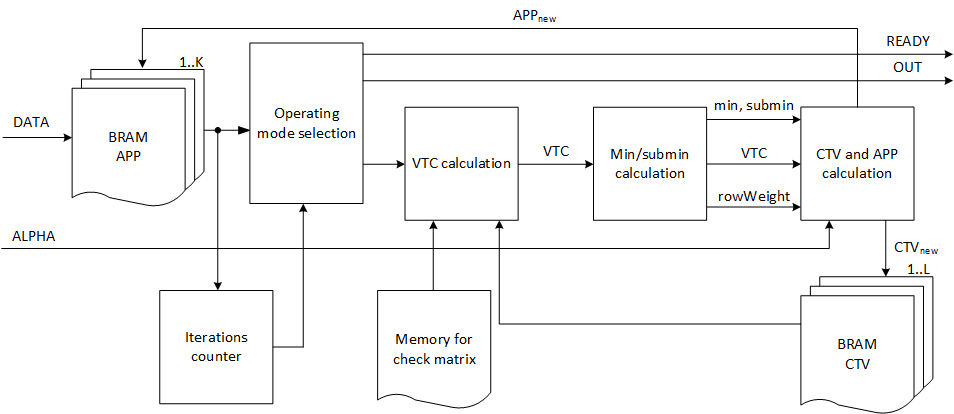
\includegraphics[width=0.9\textwidth]{./images/FPGA LDPC decoder.png}
    \caption{Kiến trúc bộ giải mã LDPC}
\end{figure}

Luồng dữ liệu bên trong bộ giải mã diễn ra theo một chu trình khép kín, được đồng bộ chặt chẽ qua từng vòng lặp:

\begin{itemize}
    \item Khởi tạo: Dòng bit dữ liệu đầu vào dạng nối tiếp được chuyển đổi thành dạng song song và ghi vào khối bộ nhớ BRAM APP. 
    \item Bắt đầu vòng lặp: Tại mỗi chu kỳ lặp, dữ liệu xác suất hậu nghiệm APP được đọc ra từ BRAM APP. Đồng thời, các thông tin về vị trí cấu trúc mạng được truy xuất từ bộ nhớ lưu trữ ma trận kiểm tra để định tuyến chính xác dữ liệu.  
    \item Tính toán VTC: Khối VTC calculation nhận APP và các giá trị CTV từ vòng lặp trước (lưu trong BRAM CTV), thực hiện phép trừ để tạo ra thông điệp VTC gửi đến các nút kiểm tra.  
    \item Tìm cực tiểu (Min/submin): Các giá trị VTC này được đẩy vào khối Min/submin calculation để tách biệt phần dấu và phần độ lớn, sau đó chạy qua một mạng lưới mạch so sánh nhằm tìm ra hai giá trị có độ lớn nhỏ nhất và nhỏ thứ hai của mỗi hàng.  
    \item Tính toán cập nhật: Khối CTV and APP calculation sử dụng các giá trị cực tiểu này, kết hợp với phép XOR các bit dấu và hệ số tỉ lệ $\alpha$ để tính ra thông điệp CTV mới ($CTV_{new}$). Ngay lập tức, khối này cộng ngược VTC với $CTV_{new}$ để tạo ra xác suất hậu nghiệm mới ($APP_{new}$).  
    \item Phản hồi và xuất dữ liệu: $APP_{new}$ được ghi đè trở lại BRAM APP và $CTV_{new}$ được ghi vào BRAM CTV cho vòng lặp tiếp theo. Nếu bộ đếm xác định đã đạt số vòng lặp tối đa, luồng dữ liệu phản hồi bị ngắt, tín hiệu READY được kích hoạt và từ mã đã được giải mã sẽ được đẩy ra đường OUT. 
\end{itemize}
\newpage
\section{Khối BRAM}
\subsection{Khối BRAM APP}
\begin{figure}[h!]
    \centering
    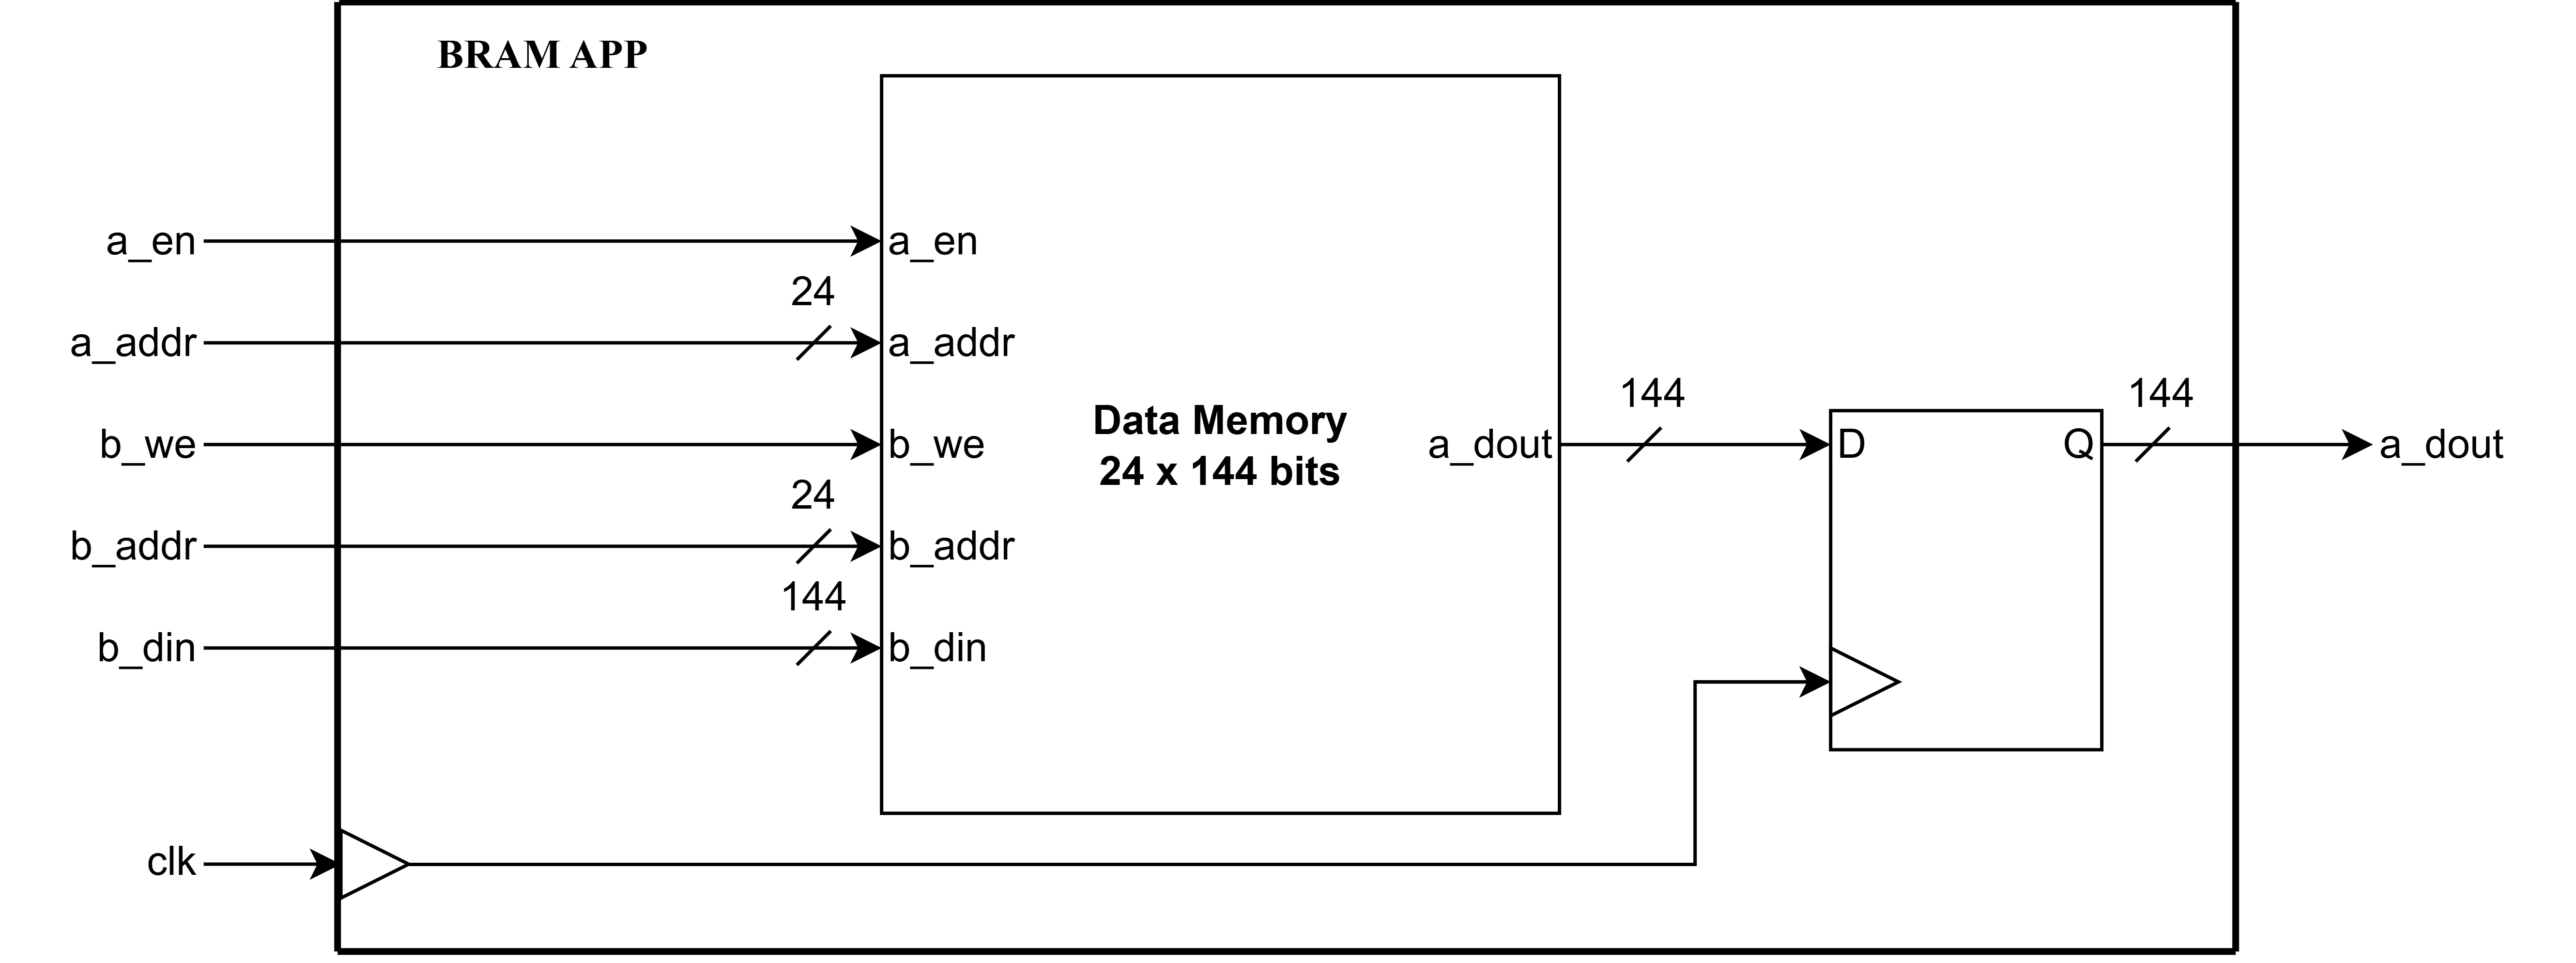
\includegraphics[width=0.9\textwidth]{./images/LDP_DECODER-BRAM_APP.drawio.png}
    \caption{Kiến trúc khối BRAM APP}
\end{figure}

Về mặt yêu cầu thiết kế, khối BRAM APP đóng vai trò chứa các giá trị APP trong suốt quá trình lặp của thuật toán Min-Sum. Các giá trị này ban đầu chính là các quyết định mềm thu được từ bộ giải điều chế của kênh truyền. Nhằm giải quyết bài toán về băng thông dữ liệu trong các thiết kế giải mã tốc độ cao, bộ nhớ này bắt buộc phải được thiết kế dưới dạng bộ nhớ RAM cổng kép (dual-port). Điều này cho phép phần cứng có thể đọc và ghi các giá trị một cách độc lập trong cùng một chu kỳ xung nhịp. 

Kiến trúc tổng quan và các thông số kỹ thuật chi tiết bao gồm:
\begin{itemize}
    \item Mã nguồn định nghĩa sẵn hai tham số cơ bản là độ sâu bộ nhớ $DEPTH = 24$ và độ rộng dữ liệu $WIDTH = 144$ bit. Không gian lưu trữ thực tế là một mảng thanh ghi hai chiều mang tên \textit{mem}.  
    \item Để hỗ trợ việc đọc và ghi song song các giá trị APP, tổng thể bộ nhớ không nằm ở một khối duy nhất mà được chia nhỏ thành $K = N/z$ khối. Trong đó, $N$ là chiều dài của từ mã và $z$ là kích thước của ma trận con tuần hoàn.
    \item Kích thước của mỗi khối BRAM APP phụ thuộc trực tiếp vào số lượng ký hiệu trong ma trận con tuần hoàn $z$ và độ rộng của dữ liệu đầu vào. Cụ thể, dung lượng được cấp phát tính bằng $(z \times \text{weight\_of\_input\_data}) \times (N/z)$.
    \item Giao tiếp Cổng A (Cổng Đọc): Cổng này chịu sự điều khiển của tín hiệu cho phép đọc \textit{a\_en}. Dữ liệu đầu ra \textit{a\_dout} được trích xuất từ vị trí \textit{a\_addr}. Giao tiếp Cổng B (Cổng Ghi): Cổng này nhận tín hiệu cho phép ghi \textit{b\_we} để nạp dữ liệu \textit{b\_din} vào địa chỉ \textit{b\_addr}.
\end{itemize}

Nguyên lý hoạt động của khối BRAM APP diễn ra như sau:
\begin{itemize}
    \item Trong pha giải mã: Tại mỗi cạnh lên của xung nhịp clk, hệ thống chỉ trích xuất một phần các khối bộ nhớ BRAM APP thông qua Cổng A. Việc khối nào được đọc hoàn toàn phụ thuộc vào cấu trúc của ma trận kiểm tra chẵn lẻ LDPC. Dữ liệu này được đẩy vào khối "VTC calculation". Đồng thời, các giá trị APP cập nhật ($APP\_{new}$) được tính toán xong sẽ ngay lập tức được ghi đè ngược lại vào bộ nhớ thông qua Cổng B.
    \item Trong pha xuất kết quả: Khi khối "Iterations counter" báo hiệu đã hoàn thành số vòng lặp tối đa, khối "Operating mode selection" sẽ chuyển trạng thái hệ thống. Lúc này, toàn bộ các khối của bộ nhớ BRAM APP sẽ được đọc và đẩy thẳng ra ngõ ra \textit{READY OUT} để cung cấp từ mã đã được giải mã hoàn chỉnh.
\end{itemize}
\subsection{Khối BRAM CTV}
\begin{figure}[h!]
    \centering
    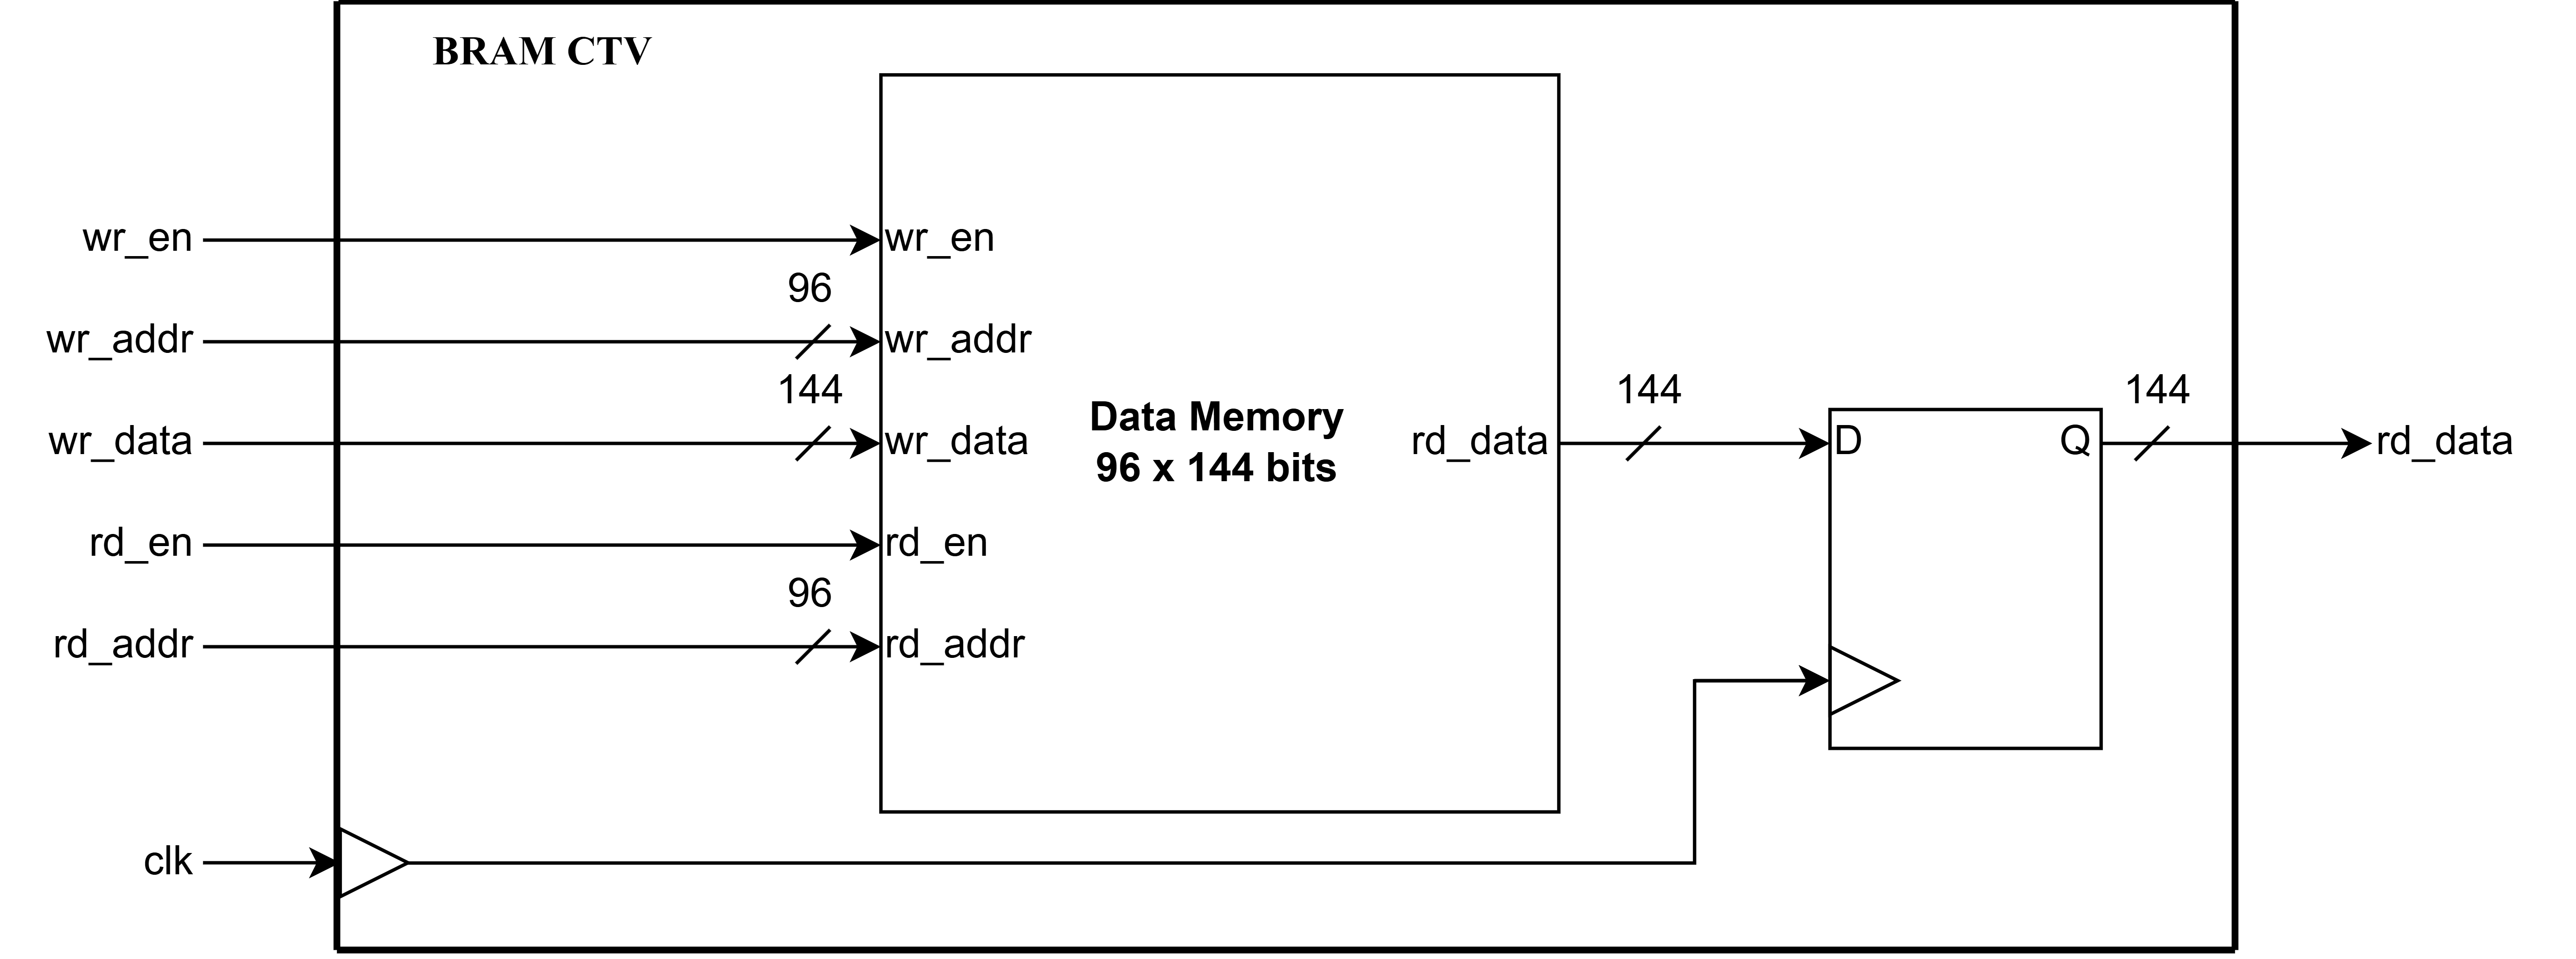
\includegraphics[width=0.9\textwidth]{./images/LDP_DECODER-BRAM_CTV.drawio.png}
    \caption{Kiến trúc khối BRAM CTV}
\end{figure}

Về mặt yêu cầu thiết kế, khối BRAM CTV là thành phần lưu trữ các bản tin CTV, tương đương với thông điệp $r\_{mn}[k]$ truyền từ nút kiểm tra $m$ đến nút biến $n$ trong thuật toán đồ thị Tanner. Vì ma trận QC-LDPC của các chuẩn WiFi (IEEE 802.11n) và WiMAX (IEEE 802.16e) có tính chất tuần hoàn, kiến trúc bộ giải mã yêu cầu phải cập nhật đồng thời tất cả các giá trị APP cho một hàng hiện tại của ma trận. Do đó, hệ thống bắt buộc phải khởi tạo $z$ phiên bản bộ nhớ CTV chạy hoàn toàn song song (với $z$ là số nhân lõi tương đương kích thước ma trận con).  

Kiến trúc tổng quan và các thông số kỹ thuật chi tiết bao gồm:
\begin{itemize}
    \item Khác với BRAM APP, dung lượng của BRAM CTV được thiết kế để tránh lãng phí tài nguyên trên FPGA. Cụ thể, độ sâu của bộ nhớ được quy định bằng đúng số lượng hàng khối nhân với trọng số hàng tối đa là $96$.
    \item Mã nguồn định nghĩa độ sâu mặc định $DEPTH = 96$ và độ rộng $WIDTH = 144$ bit. Tương đương với $z \times DW$, tức $z$ làn dữ liệu song song, mỗi làn rộng $DW$ bit.
    \item Kích thước chính xác của nhóm bộ nhớ này được ánh xạ theo cấu trúc ma trận LDPC với công thức: Trọng số hàng của ma trận $\times$ Kích thước dữ liệu đầu vào $\times$ Số lượng hàng của ma trận.
    \item Mảng thanh ghi mem được truy cập qua hai tiến trình phần cứng độc lập. Tiến trình đọc được kiểm soát bởi \textit{rd\_en, rd\_addr} để xuất \textit{rd\_data}. Tiến trình ghi được kiểm soát bởi \textit{wr\_en, wr\_addr} để nạp \textit{wr\_data}. 
\end{itemize}

Nguyên lý hoạt động của khối BRAM CTV diễn ra như sau:
\begin{itemize}
    \item Cung cấp dữ liệu (Pha Đọc): Khởi đầu mỗi chu kỳ lặp, các giá trị CTV ban đầu được thiết lập bằng 0, sau đó sẽ được xuất ra thông qua ngõ \textit{rd\_data} khi có tín hiệu \textit{rd\_en} tại cạnh lên của xung clk. Các giá trị CTV cũ này được đưa trực tiếp vào khối "VTC calculation" để thực hiện phép toán $VTC\_n = APP\_n - CTV\_n$.
    \item Cập nhật dữ liệu (Pha Ghi): Tại cuối chu trình của một hàng, khối "CTV and APP calculation" sẽ tổng hợp các giá trị VTC cực tiểu min và cực tiểu phụ submin, sau đó khối sẽ xử lý dấu (Signs XORing) để tạo ra bản tin $CTV_{new}$. Ngay lập tức, khi có xung clk và tín hiệu \textit{wr\_en} tích cực, tập dữ liệu $CTV_{new}$ này được nạp vào chân \textit{wr\_data} và ghi đè vào địa chỉ \textit{wr\_addr} tương ứng. Quá trình này đảm bảo dữ liệu luôn sẵn sàng cho vòng lặp giải mã tiếp theo.
\end{itemize}
\section{Khối Iterations Counter}
\begin{figure}[h!]
    \centering
    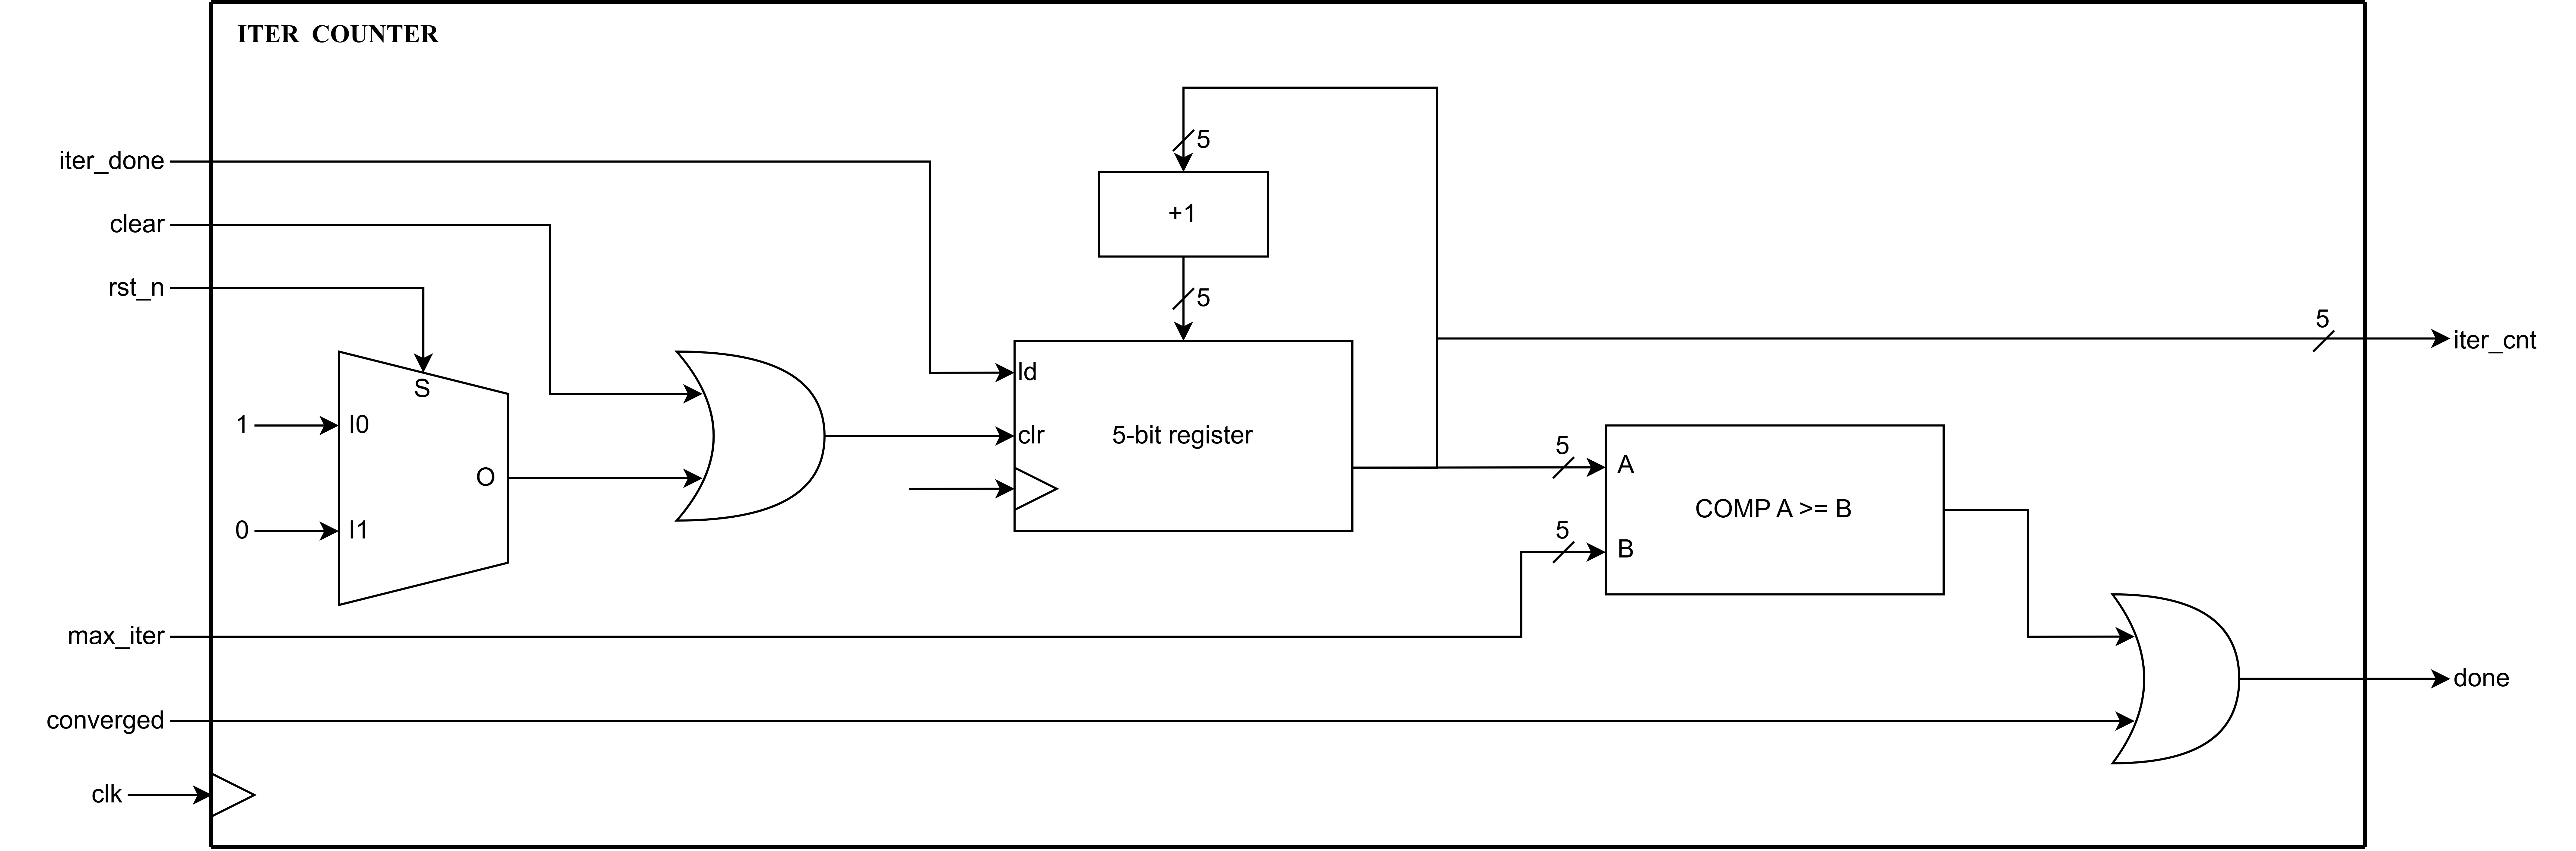
\includegraphics[width=0.9\textwidth]{./images/LDP_DECODER-ITER COUNTER.drawio.png}
    \caption{Kiến trúc khối Iterations Counter}
\end{figure}

Về mặt yêu cầu thiết kế, khối iter counter là thành phần kiểm soát số vòng lặp giải mã, tương đương với biến đếm số lần lặp trong các thuật toán lặp. Vì thuật toán giải mã yêu cầu lặp đi lặp lại quá trình cập nhật thông điệp để hội tụ, kiến trúc bộ giải mã yêu cầu phải giới hạn số vòng lặp tối đa và có khả năng dừng sớm khi đã tìm ra từ mã đúng. Do đó, hệ thống bắt buộc phải khởi tạo bộ đếm này để theo dõi tiến trình và phát tín hiệu hoàn thành (\textit{done}) chuyển khối "Operating mode selection" sang chế độ xuất kết quả. 

Kiến trúc tổng quan và các thông số kỹ thuật chi tiết bao gồm:
\begin{itemize}
    \item Khác với các khối lưu trữ dữ liệu, khối iter counter được thiết kế dưới dạng một bộ đếm đồng bộ kết hợp logic tổ hợp để tránh giải mã mắc kẹt trong vòng lặp vô tận.
    \item Mã nguồn định nghĩa độ rộng mặc định \textit{ITER\_W} = 5 bit và cờ cho phép dừng sớm \textit{DONE} = 1. Tương đương với việc phần cứng có thể đếm và quản lý tối đa 32 vòng lặp, mỗi vòng được biểu diễn trên 5 bit dữ liệu. 
    \item Giới hạn lặp chính xác của hệ thống được ánh xạ theo cấu hình động với đầu vào \textit{max\_iter} có độ rộng \textit{ITER\_W} bit, quy định số vòng lặp tối đa cho từng phiên chạy.
    \item Khối đếm được cập nhật qua một tiến trình phần cứng tuần tự độc lập. Tiến trình này được kiểm soát bởi tín hiệu đồng hồ clk và tín hiệu reset không đồng bộ \textit{rst\_n} để xuất ra giá trị vòng lặp hiện tại \textit{iter\_cnt} và cờ trạng thái done.
\end{itemize}

Nguyên lý hoạt động của khối iter counter diễn ra như sau:
\begin{itemize}
    \item Khởi tạo và làm mới dữ liệu (Pha Khởi tạo): Khởi đầu hệ thống (tín hiệu \textit{rst\_n} ở mức thấp) hoặc khi hệ thống bắt đầu xử lý một khung giải mã mới (tín hiệu clear tích cực), các giá trị của bộ đếm \textit{iter\_cnt} và cờ \textit{done} ban đầu được thiết lập bằng 0.
    \item Cập nhật và đánh giá (Pha Đếm): Tại quá trình giải mã, khi có xung \textit{iter\_done} báo hiệu kết thúc một vòng lặp, khối sẽ thực hiện phép toán \textit{iter\_cnt} + 1'b1 để tăng biến đếm. Ngay lập tức, khối sẽ tổng hợp các điều kiện để xét duyệt hoàn thành: nếu giá trị lặp tiếp theo đạt tới ngưỡng \textit{max\_iter} hoặc nếu cờ \textit{DONE} tích cực đi kèm với việc bật sáng sớm thì tín hiệu \textit{done} sẽ được nạp mức cao. Quá trình này đảm bảo tín hiệu hoàn thành luôn sẵn sàng để hệ thống dừng giải mã đúng thời điểm. 
\end{itemize}

\section{Khối Operating Mode Selection}
Trong hệ thống bộ giải mã LDPC, quá trình giải mã thông thường sẽ kết thúc khi toàn bộ từ mã thỏa mãn phương trình kiểm tra chẵn lẻ $Hx = 0$, hoặc khi mạch đếm vòng lặp đạt đến giới hạn số vòng lặp tối đa được thiết lập từ trước. Dựa trên nguyên lý đó, khối \texttt{mode\_select\_top} được thiết kế theo cấu trúc phân rã nhằm quản lý việc chuyển đổi trạng thái giữa quá trình lặp và quá trình xuất dữ liệu. Thiết kế này tách biệt rõ ràng luồng điều khiển (đếm vòng lặp, kiểm tra điều kiện dừng) và luồng định tuyến dữ liệu thông qua 5 module con hoạt động phối hợp như sau:

\textbf{Khối đếm vòng lặp (\texttt{iteration\_counter}):} Đây là một mạch tuần tự chịu trách nhiệm theo dõi số lượng vòng lặp hiện tại của bộ giải mã. Thay vì sử dụng toán tử cộng (\texttt{+}) thông thường, module này tái sử dụng khối tính toán toán học lõi \texttt{fa\_calc} với chân chọn chế độ $Sel = 0$ (tương đương phép cộng) nhằm đồng bộ hóa việc sử dụng tài nguyên với các module khác trong hệ thống. Khi tín hiệu \texttt{enable} ở mức cao, giá trị bộ đếm được cập nhật:
\begin{equation}
    count\_plus\_one = count + 1
\end{equation}
Bên cạnh đó, mạch được trang bị cờ \texttt{start} kết hợp với reset bất đồng bộ (\texttt{reset\_n}), cho phép hệ thống chủ động khởi tạo lại số đếm về 0 khi bắt đầu xử lý một khung dữ liệu mới.

\begin{figure}[h!]
    \centering
    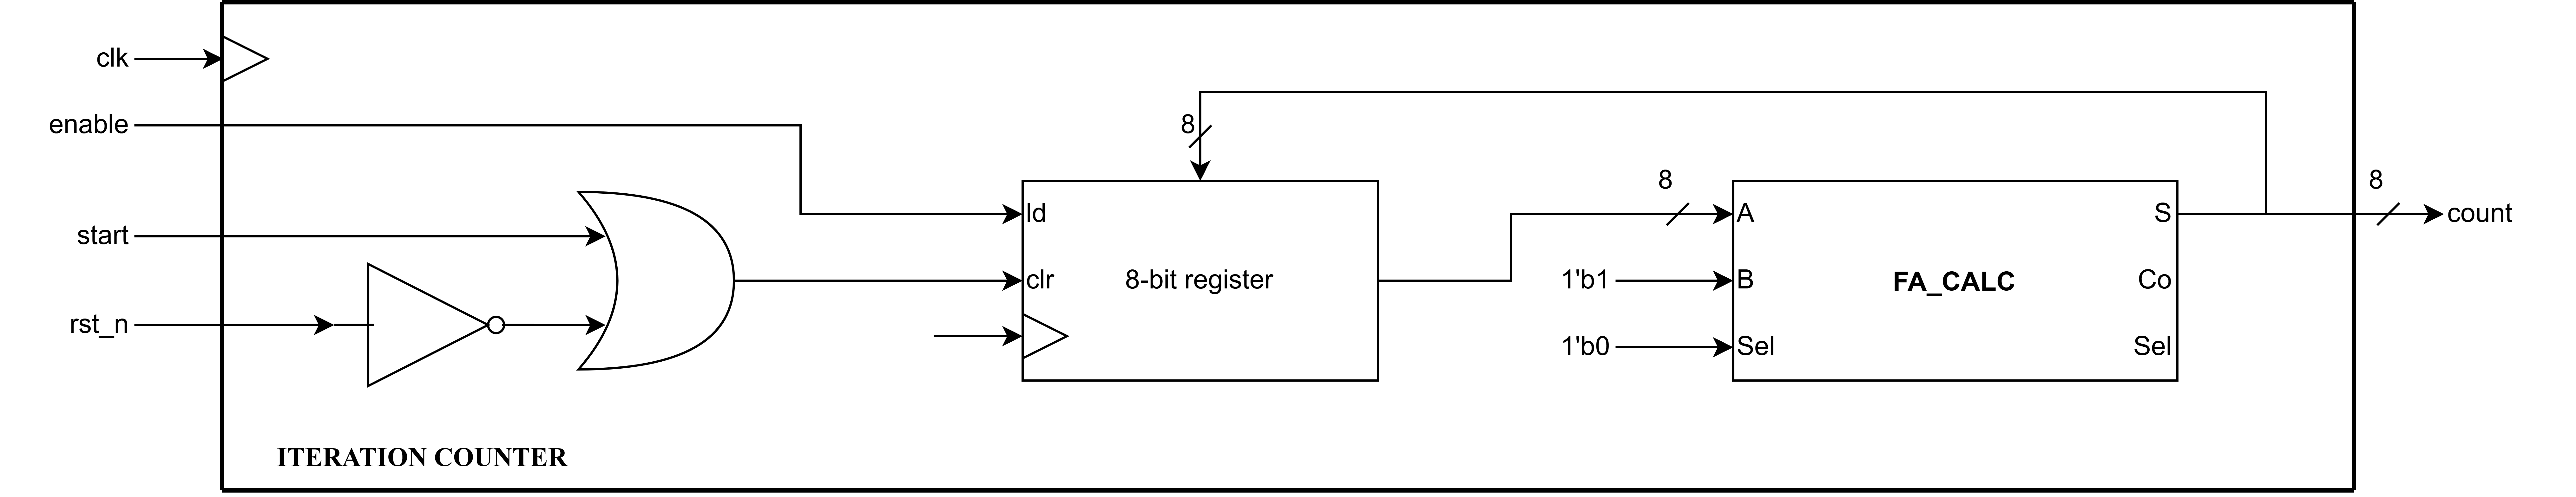
\includegraphics[width=0.9\textwidth]{./images/LDP_DECODER-MODE_SELECT.drawio (1).png}
    \caption{Kiến trúc khối Iterations Counter}
\end{figure}

\textbf{Khối so sánh điều kiện dừng (\texttt{iter\_compare}):} Mô-đun này có nhiệm vụ phát hiện thời điểm bộ giải mã đã đạt đến ngưỡng $max\_iteration$. Để tối ưu hóa cổng logic, mạch tiếp tục sử dụng khối \texttt{fa\_calc} nhưng được cấu hình như một bộ trừ ($Sel = 1$). Bằng cách thực hiện phép trừ giữa số vòng lặp hiện tại và giới hạn tối đa, tín hiệu hoàn tất (\texttt{done}) được trích xuất trực tiếp thông qua cờ nhớ $C_o$:
\begin{equation}
    done = C_o (iteration\_count - max\_iteration)
\end{equation}
Ngay khi $iteration\_count$ bằng hoặc vượt mức $max\_iteration$, cờ tràn $C_o$ sẽ lên mức 1, báo hiệu hệ thống cần kết thúc quá trình lặp.
\newpage

\begin{figure}[h!]
    \centering
    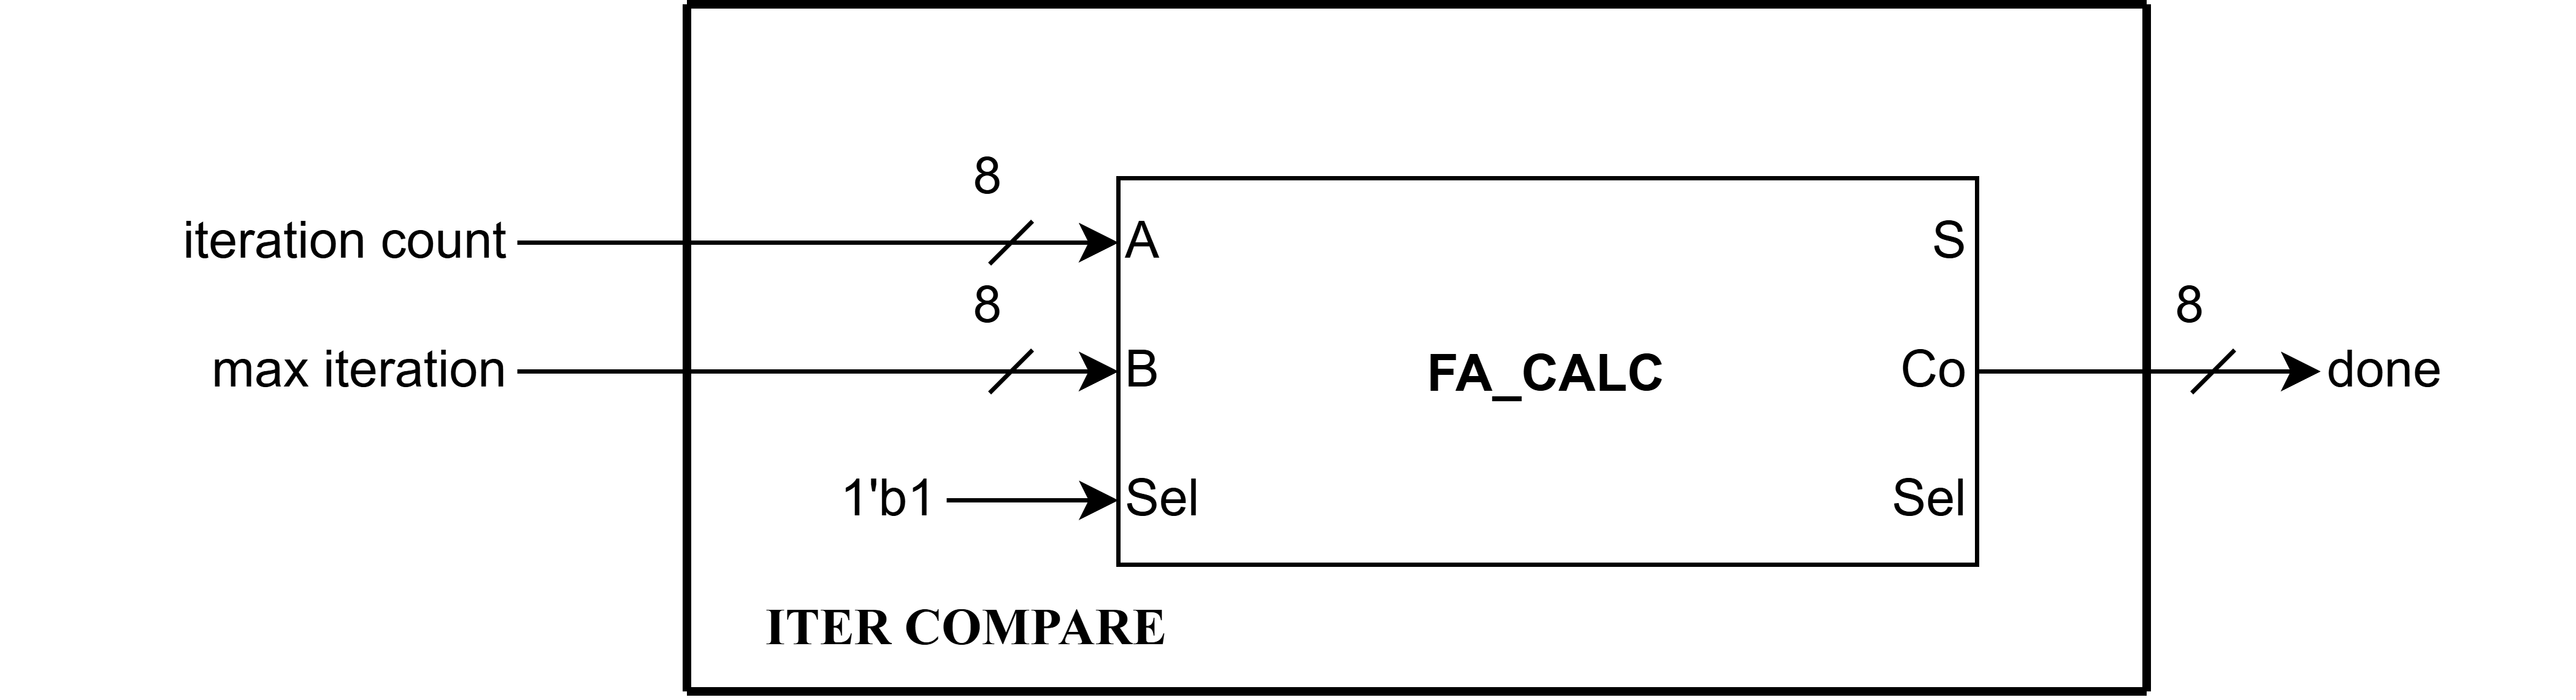
\includegraphics[width=0.8\textwidth]{./images/LDP_DECODER-MODE_SELECT.drawio.png}
    \caption{Kiến trúc khối Iterations Compare}
\end{figure}

\textbf{Khối giao diện mức cao nhất (\texttt{mode\_select\_top}):} Module \texttt{mode\_select\_top} thực hiện chức năng wrapper. Việc đóng gói khối dãy (\texttt{iteration\_counter}) cùng với các khối tổ hợp (\texttt{iter\_compare}) thành một IP duy nhất giúp thiết lập ranh giới rõ ràng cho kiến trúc. Điều này tạo thuận lợi cho việc synthesis, đồng thời giúp công cụ thiết kế dễ dàng đánh giá timing analysis của toàn bộ module mà không bị nhiễu bởi các khối bên ngoài. 

\begin{figure}[h!]
    \centering
    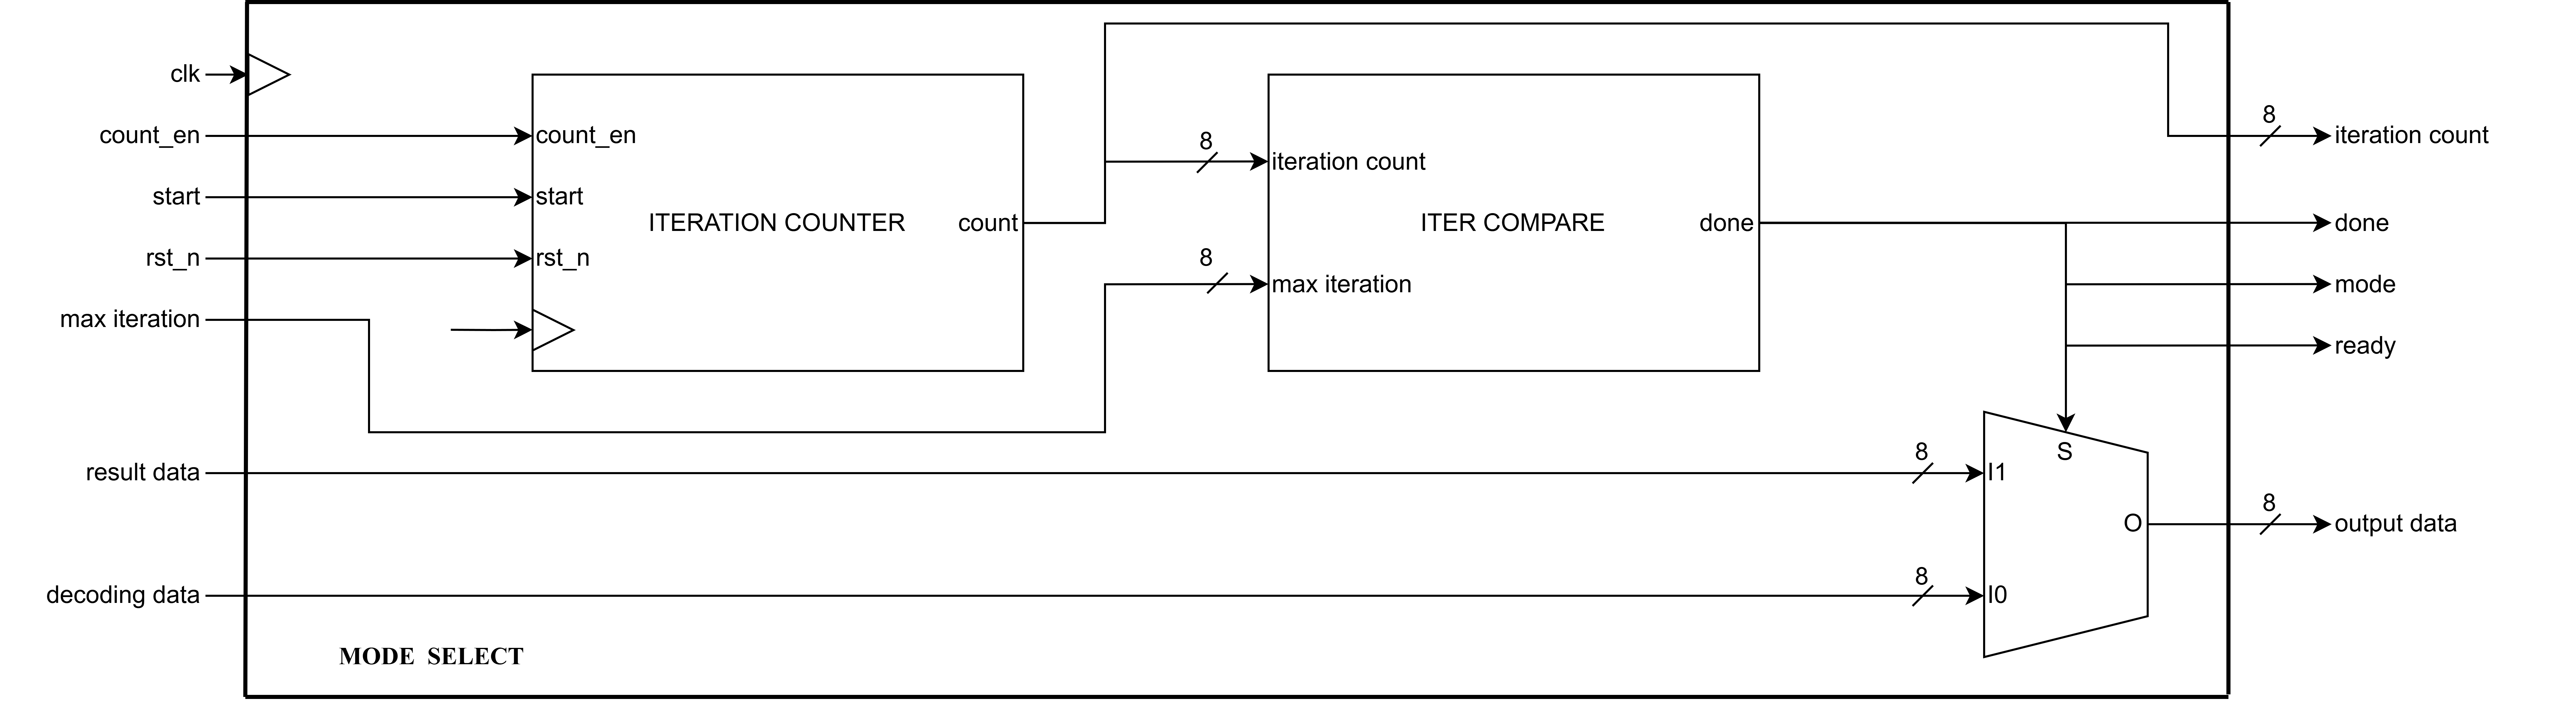
\includegraphics[width=\textwidth]{./images/LDP_DECODER-MODE_SELECT.drawio (2).png}
    \caption{Kiến trúc khối Mode Select}
\end{figure}

\textbf{Bộ định tuyến dữ liệu:} Đóng vai trò là một bộ ghép kênh 2-to-1 thuần tổ hợp. Chức năng chính của bộ này là lựa chọn nguồn dữ liệu ngõ ra dựa vào tín hiệu cờ trạng thái \texttt{mode}:
\begin{align}
    output\_data &= \begin{cases}
        result\_data & \text{nếu } mode = 1 \\
        decoding\_data & \text{nếu } mode = 0
    \end{cases}
\end{align}
Kiến trúc này đảm bảo mạch luôn giữ ổn định luồng dữ liệu trung gian (\texttt{decoding\_data}) trong suốt quá trình giải mã, và chỉ chuyển qua luồng đầu ra cuối cùng (\texttt{result\_data}) khi hệ thống nhận được lệnh kết thúc.

\textbf{Bộ quản lý trạng thái trung gian:} Đây là cầu nối đảm nhận vai trò liên kết logic điều khiển (\texttt{iter\_compare}) và phần tử định tuyến datapath (\texttt{mode\_mux}). Nó tiếp nhận cờ \texttt{done} từ bộ so sánh và phân phối thành các tín hiệu điều khiển toàn cục, bao gồm \texttt{mode} và \texttt{ready} dùng để thông báo cho các khối xử lý ở tầng cao hơn về trạng thái dữ liệu:
\begin{equation}
    mode = ready = done
\end{equation}

\section{Khối VTC Calculation}
\begin{figure}[h!]
    \centering
    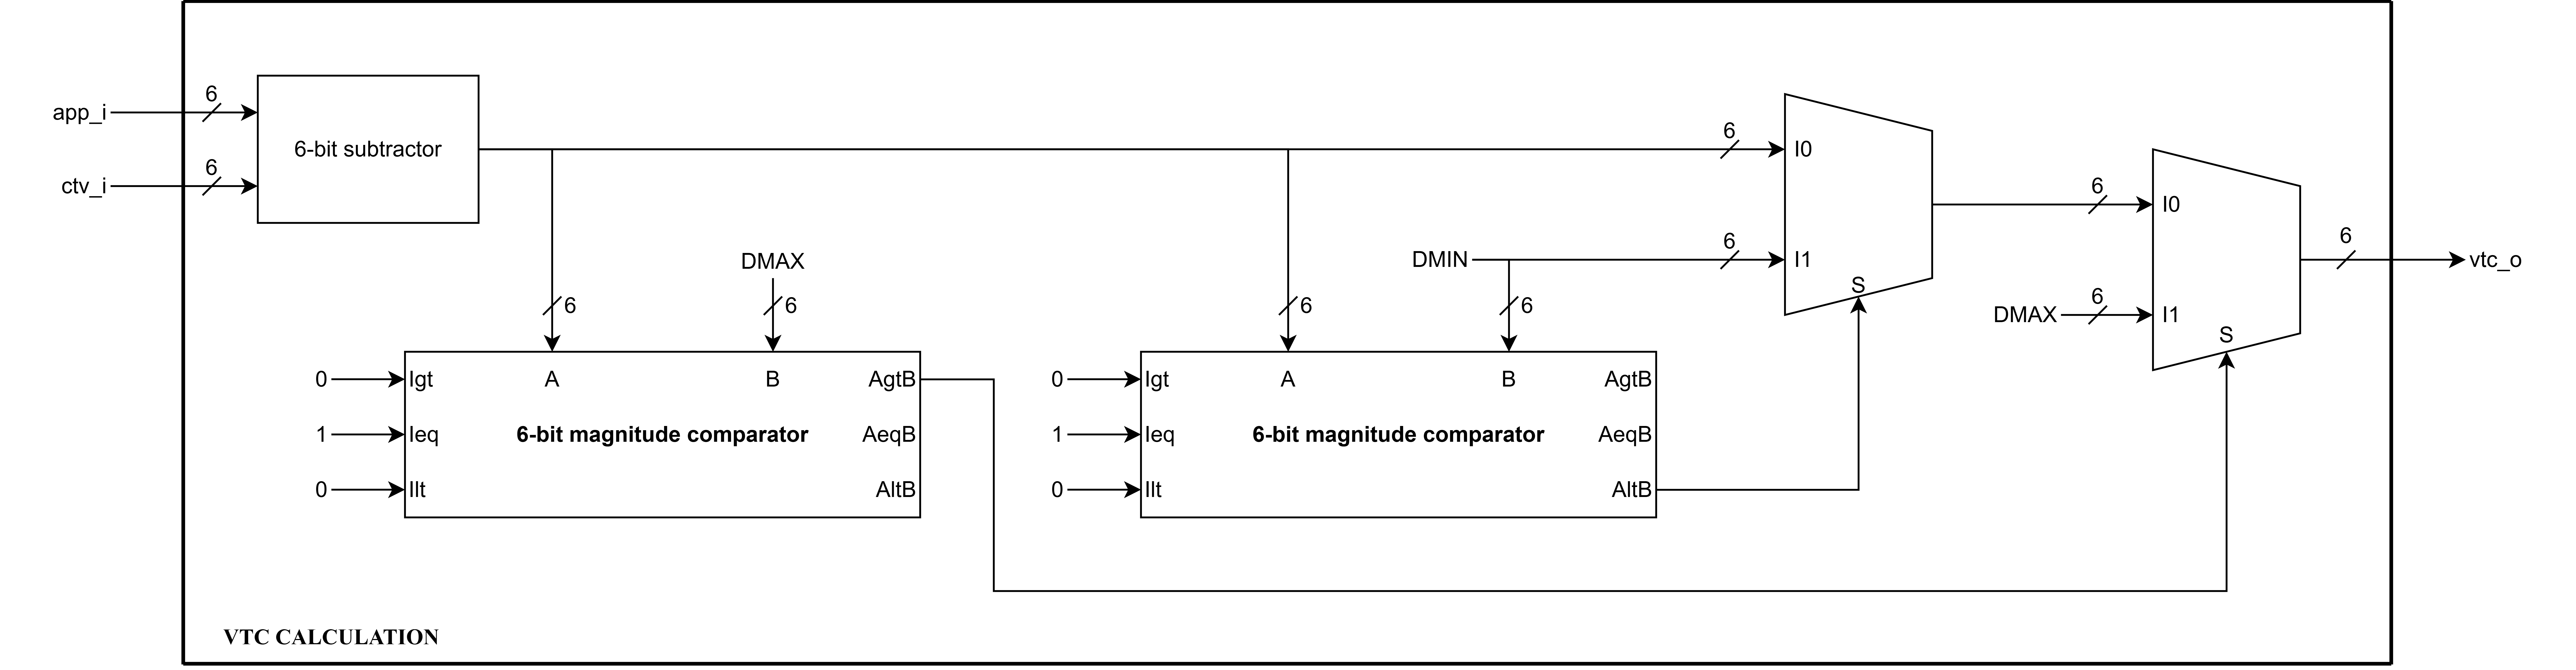
\includegraphics[width=\textwidth]{./images/LDP_DECODER-VTC_CALC.drawio.png}
    \caption{Kiến trúc khối VTC Calculation}
\end{figure}

Khối VTC calculation chịu trách nhiệm tính toán các thông điệp VTC trong cấu trúc của bộ giải mã LDPC. Khối này nhận đầu vào là các giá trị xác suất hậu nghiệm APP từ khối bộ nhớ BRAM APP. Dựa trên APP và giá trị thông điệp CTV tương ứng, khối sẽ tính toán ra tín hiệu VTC. Đầu ra VTC sau đó sẽ được chuyển tiếp đến khối tính toán Min/submin để thực hiện các bước tiếp theo của thuật toán giải mã Min-Sum. Khối được thiết kế để xử lý song song, trong đó số lượng bộ xử lý tương đương với kích thước ma trận con $Z$, cho phép cập nhật đồng thời tất cả các giá trị APP được sử dụng bởi hàng hiện tại của ma trận kiểm tra. Nguyên lý hoạt động của khối dựa trên việc hiện thực hóa công thức tính toán bản tin VTC ~\ref{eq:2}.

Trong phần cứng, các bản tin APP được biểu diễn dưới dạng số nguyên có dấu với độ rộng $DW = 8$ bit. Phép trừ trực tiếp giữa hai số có dấu dễ dẫn đến hiện tượng tràn số, khiến một giá trị mang độ tin cậy cao bị đảo dấu thành độ tin cậy thấp. Để khắc phục, thiết kế tích hợp mạch trừ bão hòa kẹp giá trị ngõ ra trong dải $[-128, 127]$ theo logic:
\begin{equation}
    VTC_o[i] = 
    \begin{cases} 
        D_{MAX}, & \text{nếu } (APP_i - CTV_i) > D_{MAX} \\
        D_{MIN}, & \text{nếu } (APP_i - CTV_i) < D_{MIN} \\
        APP_i - CTV_i, & \text{ngược lại}
    \end{cases}
\end{equation}
Đối với trường hợp thiết kế tham số $DW = 8$ bit, hai ngưỡng giới hạn bão hòa được xác định là $D_{MAX} = +127$ và $D_{MIN} = -128$.

\begin{figure}[h!]
    \centering
    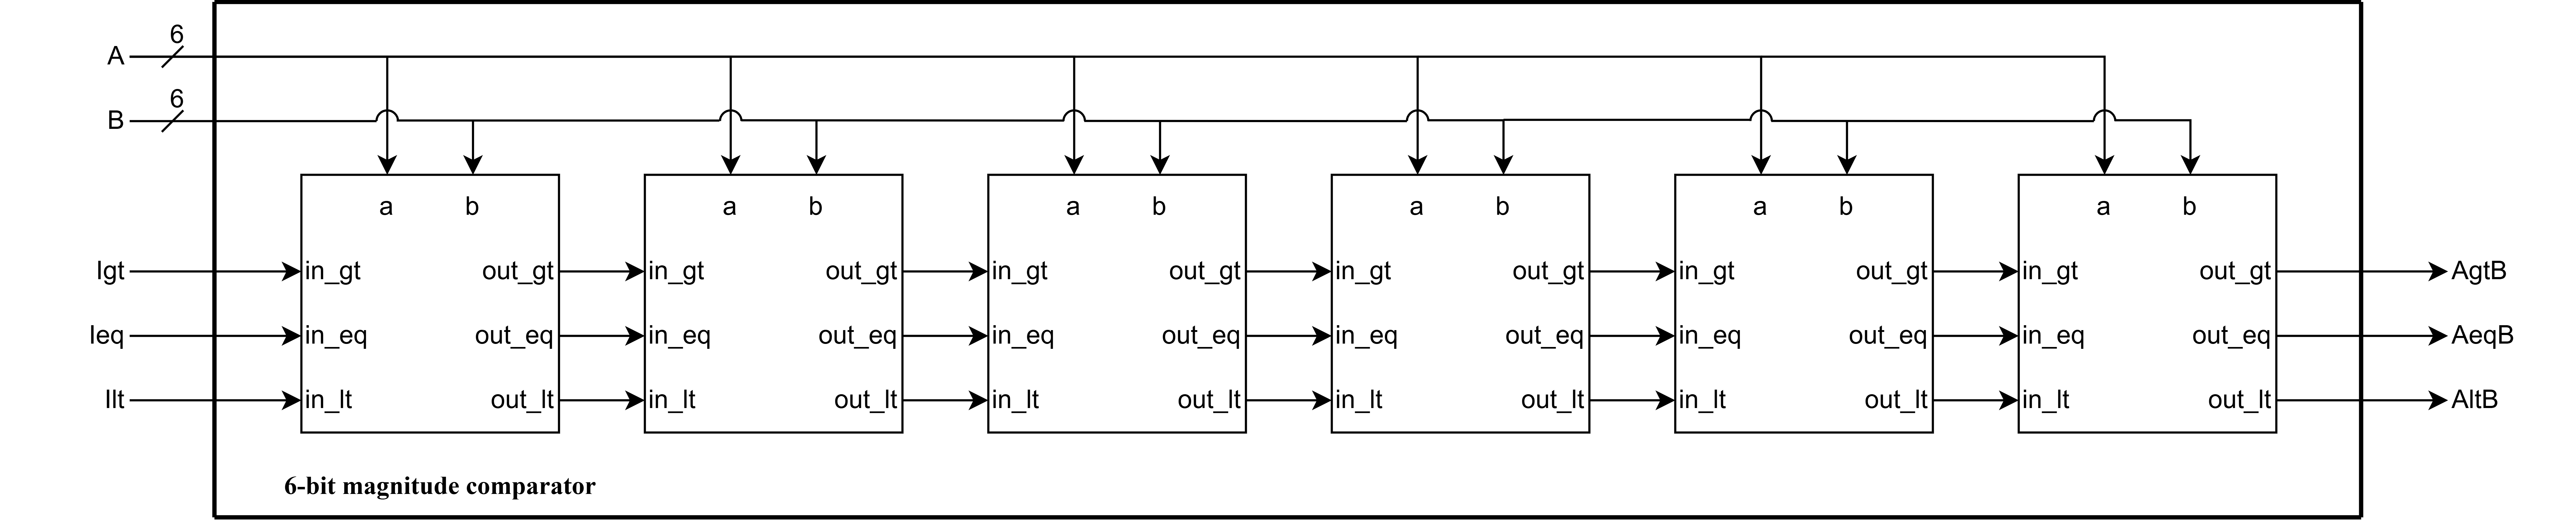
\includegraphics[width=\textwidth]{./images/LDP_DECODER-VTC_CALC(1).drawio.png}
    \caption{Kiến trúc Bộ so sánh độ lớn số 6 bit}
\end{figure}

Kiến trúc phần cứng mức logic của khối \texttt{vtc\_calc} được hiện thực hóa thông qua các thành phần liên kết chặt chẽ:
\begin{itemize}
    \item \textbf{Bộ trừ có dấu 6-bit:} Thực hiện phép trừ giữa hai làn dữ liệu ngõ vào $diff = APP_i - CTV_i$. Giá trị hiệu số $diff$ được mở rộng dải bit trung gian nhằm đảm bảo không mất mát thông tin bit dấu khi xảy ra tràn số.
    \item \textbf{Chuỗi bộ so sánh độ lớn 6-bit (6-bit Magnitude Comparator):} Tín hiệu hiệu số $diff$ được đưa song song vào hai bộ so sánh 6-bit để kiểm tra điều kiện bão hòa:
    \begin{itemize}
        \item Bộ so sánh thứ nhất đối chiếu $diff$ với ngưỡng cực đại $D_{MAX} = +31$.
        \item Bộ so sánh thứ hai đối chiếu $diff$ với ngưỡng cực tiểu $D_{MIN} = -32$.
    \end{itemize}
    Mỗi bộ so sánh độ lớn 6-bit được cấu tạo từ một chuỗi nối tầng của 6 ô so sánh 1-bit từ bit có trọng số cao nhất MSB đến bit thấp nhất LSB. Tại mỗi bit $i$, ô so sánh tiếp nhận hai bit dữ liệu đầu vào $a_i, b_i$ cùng các cờ trạng thái từ tầng trước là $in\_gt, in\_eq, in\_lt$ để cập nhật cờ ngõ ra $out\_gt, out\_eq, out\_lt$ theo các biểu thức Boolean:
    \begin{align}
        out\_gt &= in\_gt \lor (in\_eq \land a_i \land \bar{b}_i) \\
        out\_eq &= in\_eq \land \overline{(a_i \oplus b_i)} \\
        out\_lt &= in\_lt \lor (in\_eq \land \bar{a}_i \land b_i)
    \end{align}
    \item \textbf{Bộ dồn kênh MUX:} Tín hiệu điều khiển ngõ ra $AgtB$ và $AltB$ từ các bộ so sánh 6-bit sẽ điều khiển mạng MUX chọn lựa giá trị xuất ra $VTC_o$. Nếu phát hiện tràn trên ($diff > D_{MAX}$), MUX chuyển ngõ ra về $D_{MAX}$; nếu tràn dưới ($diff < D_{MIN}$), ngõ ra chọn $D_{MIN}$; trường hợp không tràn, giá trị hiệu $diff$ ban đầu được truyền trực tiếp ra ngõ ra.
\end{itemize}

\section{Khối Min/Submin Calculation}
Khối \texttt{min\_submin\_calc} đóng vai trò là lõi toán học trung tâm của quá trình cập nhật nút kiểm tra trong thuật toán MSA của bộ giải mã LDPC. Đối với một hàng có trọng số $d_r = 7$ (nhận 7 bản tin đầu vào), chức năng cốt lõi của khối là xử lý tập hợp các bản tin $VTC$ để tạo ra các bản tin $CTV$ phản hồi. 

Để tối ưu hóa tài nguyên và tăng cường hiệu năng trên FPGA/ASIC, thiết kế phần cứng của khối xử lý nút kiểm tra này được phân rã thành các module con hoạt động theo chuỗi dữ liệu, được xây dựng từ các khối tính toán cơ sở bao gồm bộ cộng toàn phần \texttt{fa}, bộ toán học \texttt{fa\_calc}, và bộ so sánh \texttt{comp\_min}.

\begin{figure}[h!]
    \centering
    
\includegraphics[width=\textwidth]{./images/LDP_DECODER-ABS.drawio.png}
    \caption{Kiến trúc phần tử con full adder 8 bit}
\end{figure}

\textbf{Khối tách dấu và biên độ (\texttt{abs\_calc}):} Bước đầu tiên của thuật toán Min-Sum yêu cầu tách bản tin $VTC$ (biểu diễn dưới dạng số có dấu bù 2 - 8 bit) thành hai thành phần độc lập: bít dấu (sign) và biên độ (magnitude). Khối này sử dụng các bộ tính toán \texttt{fa\_calc} (dựa trên chuỗi nối tiếp các bộ cộng toàn phần \texttt{fa}) để thực hiện việc chuyển đổi bù 2 nếu dữ liệu là số âm. Với tín hiệu chọn $Sel$ được gán bằng bít có trọng số cao nhất (MSB), biên độ $y_i$ và bít dấu $sign\_o_i$ được xác định theo biểu thức:
\begin{align}
    sign\_o_i &= x_i[7] \nonumber \\
    y_i &= \begin{cases} 
        x_i & \text{nếu } sign\_o_i = 0 \\
        \sim x_i + 1 & \text{nếu } sign\_o_i = 1 
    \end{cases}
\end{align}
\textit{(Lưu ý: Phép toán $\sim x_i + 1$ được thực hiện tối ưu bằng cách đưa tín hiệu MSB vào chân Carry-in ($C_i$) và cổng XOR của \texttt{fa\_calc}).}

\begin{figure}[h!]
    \centering
    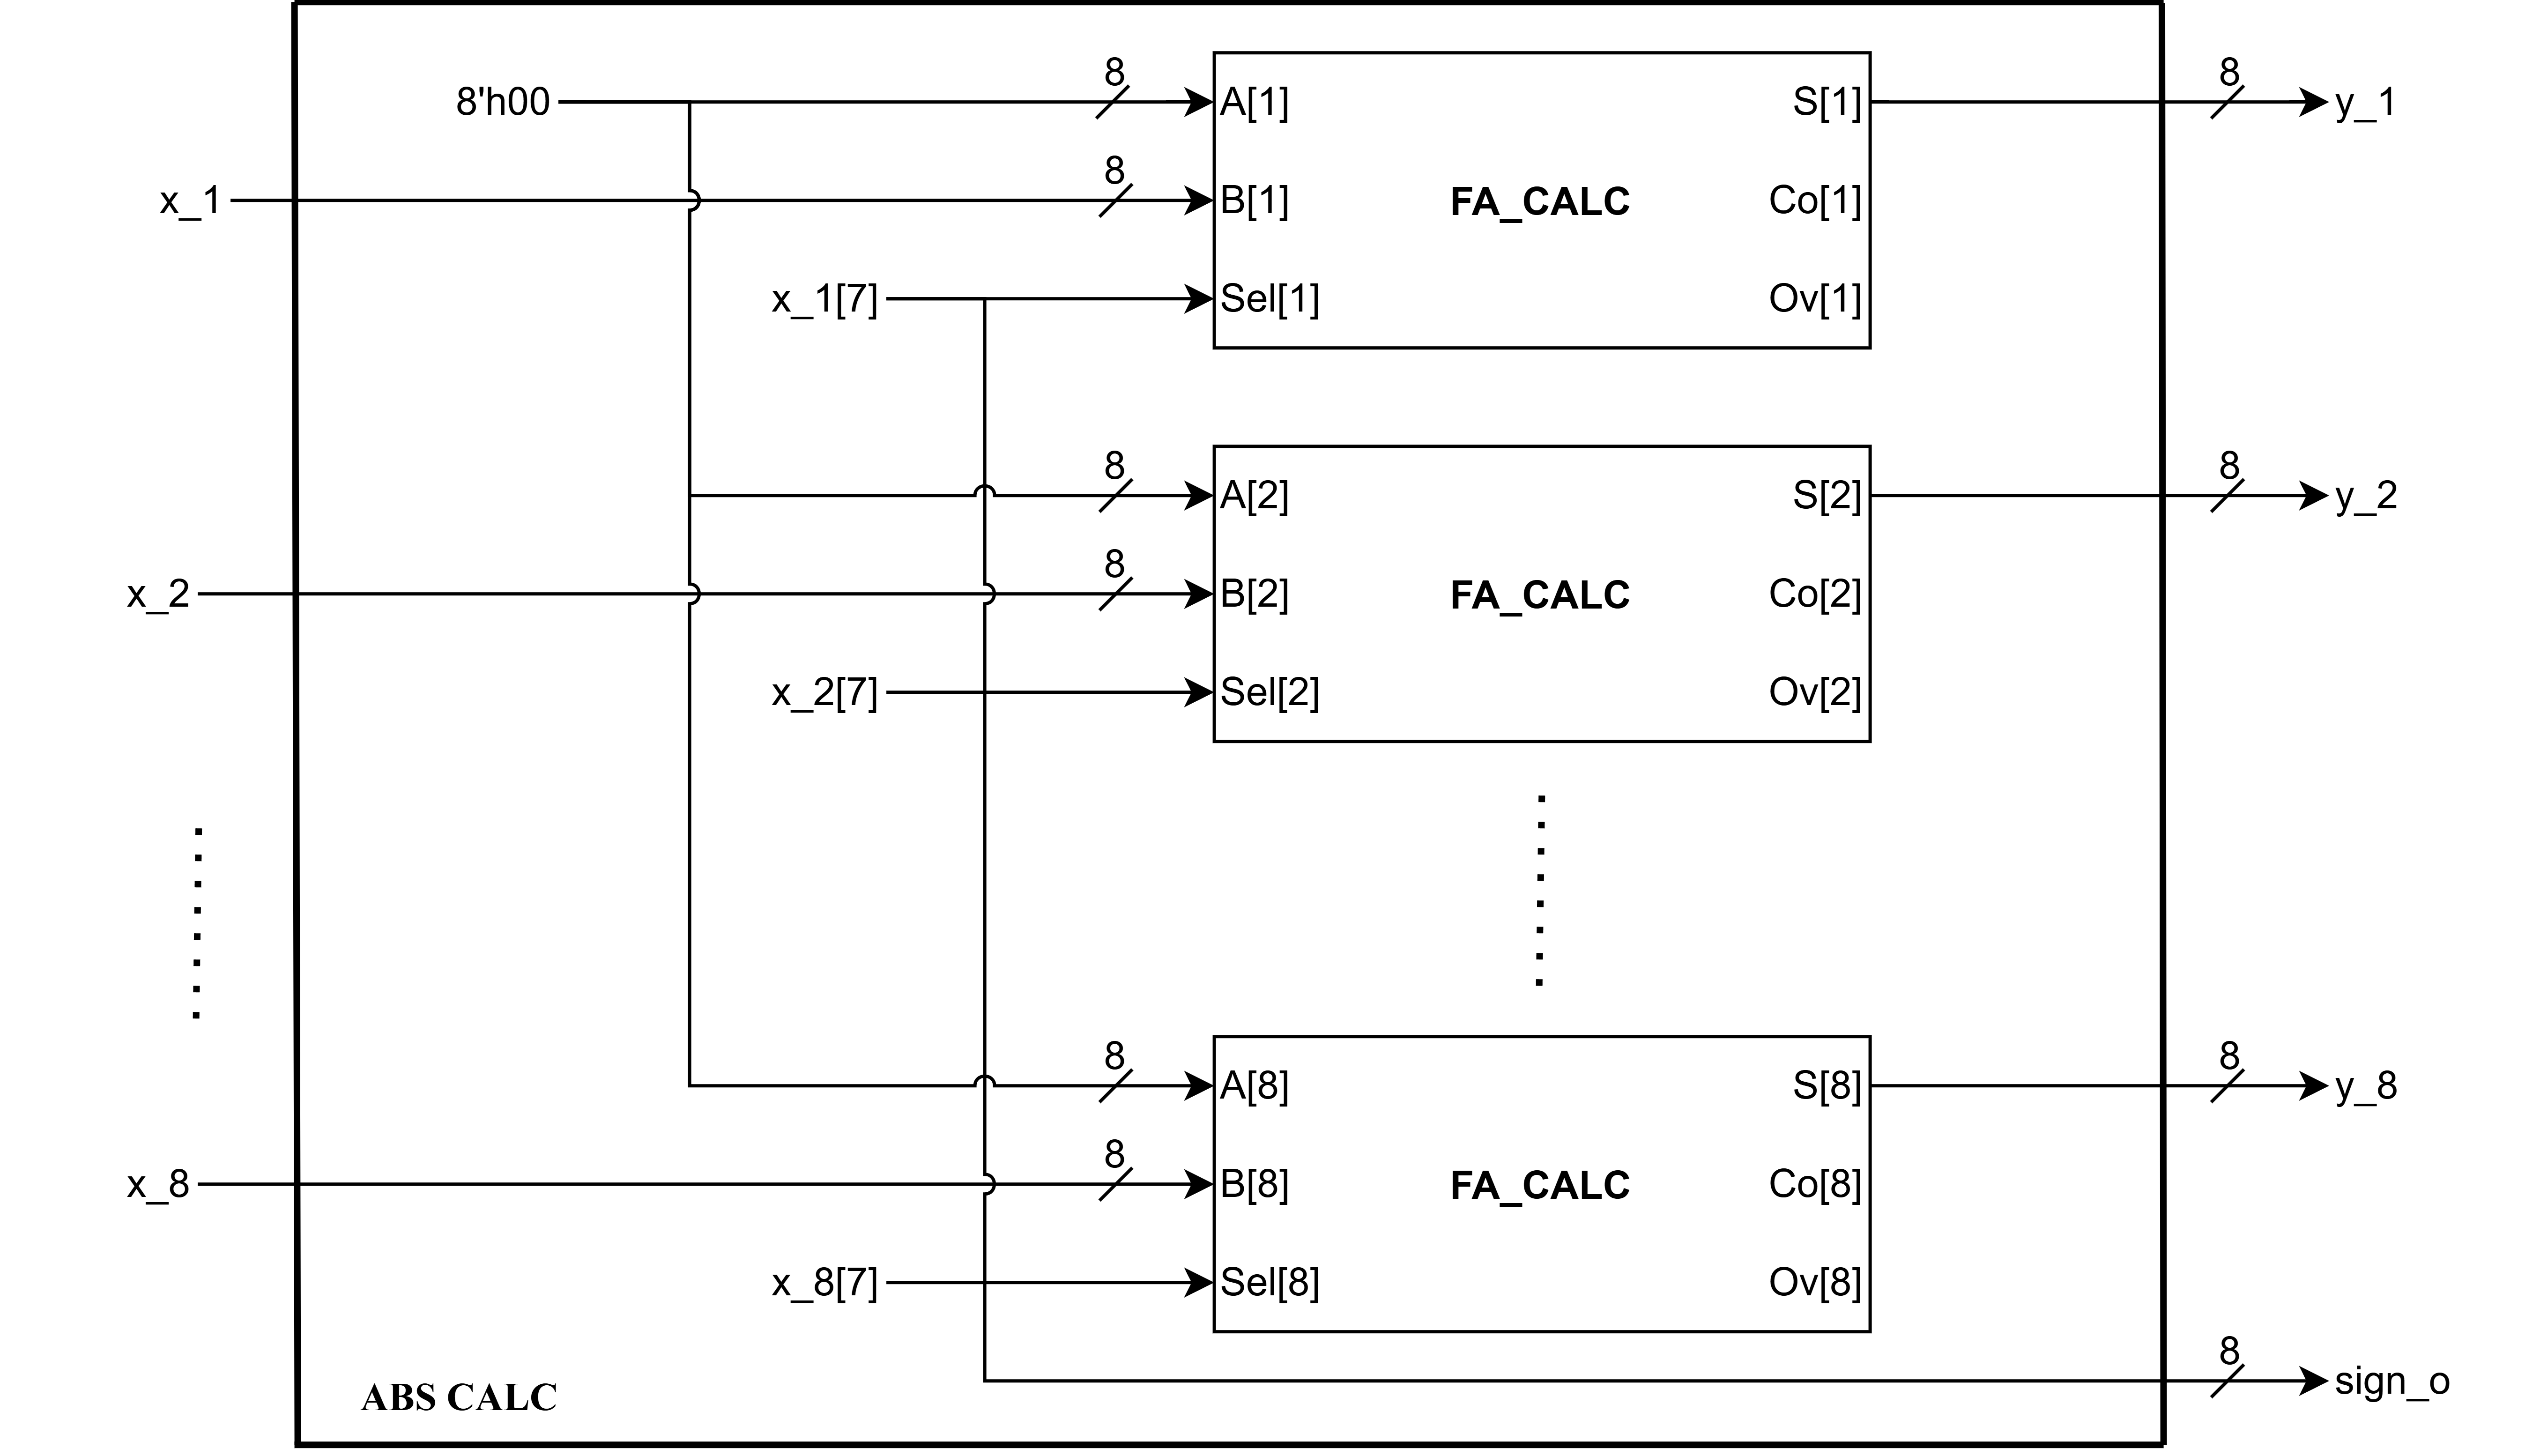
\includegraphics[width=0.8\textwidth]{./images/LDP_DECODER-ABS.drawio (1).png}
    \caption{Kiến trúc Khối ABS}
\end{figure}

\textbf{Khối tính toán bít dấu tổng (\texttt{signs\_xoring}):} Đồng thời với quá trình xử lý biên độ, các bít dấu của 7 bản tin đầu vào được đưa qua một chuỗi các cổng XOR để tìm ra bít dấu tích lũy toàn cục ($sign\_total$). Điểm đặc biệt trong thiết kế phần cứng ở đây là việc tái sử dụng cấu trúc bộ cộng toàn phần (\texttt{fa}) với chân $C_{in} = 0$, biến chân $Sum$ thành cổng XOR 2 ngõ vào để tạo thành một chuỗi XOR liên tiếp:
\begin{equation}
    sign\_total = \bigoplus_{i=1}^{7} sign\_o_i
\end{equation}

\begin{figure}[h!]
    \centering
    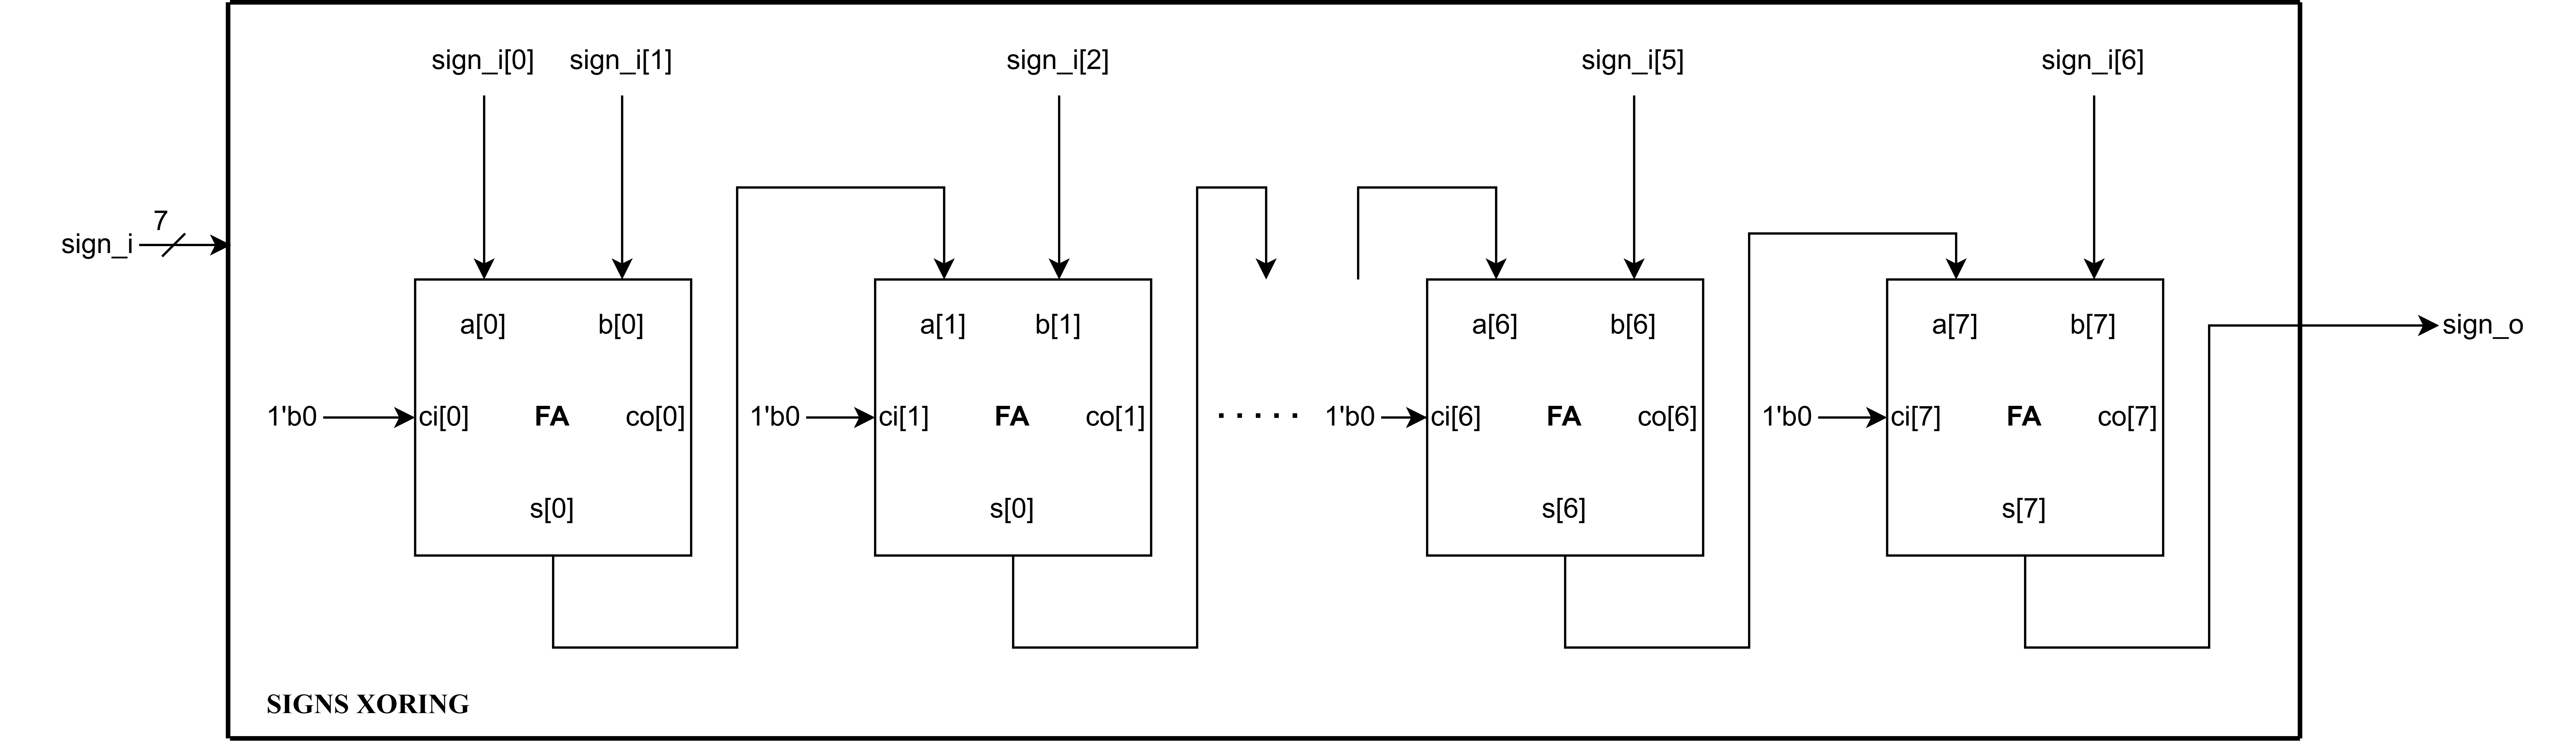
\includegraphics[width=0.9\textwidth]{./images/LDP_DECODER-ABS.drawio (2).png}
    \caption{Kiến trúc Khối SignsXoring}
\end{figure}

\textbf{Cây so sánh tìm biên độ cực tiểu (\texttt{comp\_tree} \& \texttt{comp\_min}):} Đây là thành phần đóng vai trò tìm giá trị biên độ nhỏ nhất (Min) và nhỏ nhì (Submin) để phân phối lại cho các ngõ ra. Thay vì duyệt tuần tự, thiết kế sử dụng cấu trúc cây so sánh được xây dựng từ 18 bộ \texttt{comp\_min}. 
    
Bộ \texttt{comp\_min} thực hiện phép trừ $A - B$ thông qua \texttt{fa\_calc} (với $Sel = 1$). Dựa vào cờ tràn $C_o$, phần cứng sẽ quyết định giá trị nhỏ hơn. Cây so sánh này không chỉ tìm ra giá trị cực tiểu toàn cục ($min\_all$), mà còn tính toán trước giá trị biên độ sẽ được gửi trả về cho từng nhánh thứ $i$ (gọi là $y_i$) theo nguyên tắc loại trừ chính nó:
\begin{align}
    y_i &= \min_{j \in \{1..7\}, j \neq i} \left( |VTC_j| \right)
\end{align}
Giá trị ngõ ra $y_i$ sẽ chính là cực tiểu thứ nhất ($min\_1$) nếu ngõ vào $x_i$ không phải là cực tiểu thứ nhất, và sẽ là cực tiểu thứ hai ($min\_2$ hay submin) nếu $x_i$ chính là giá trị cực tiểu thứ nhất. 

\begin{figure}[h!]
    \centering
    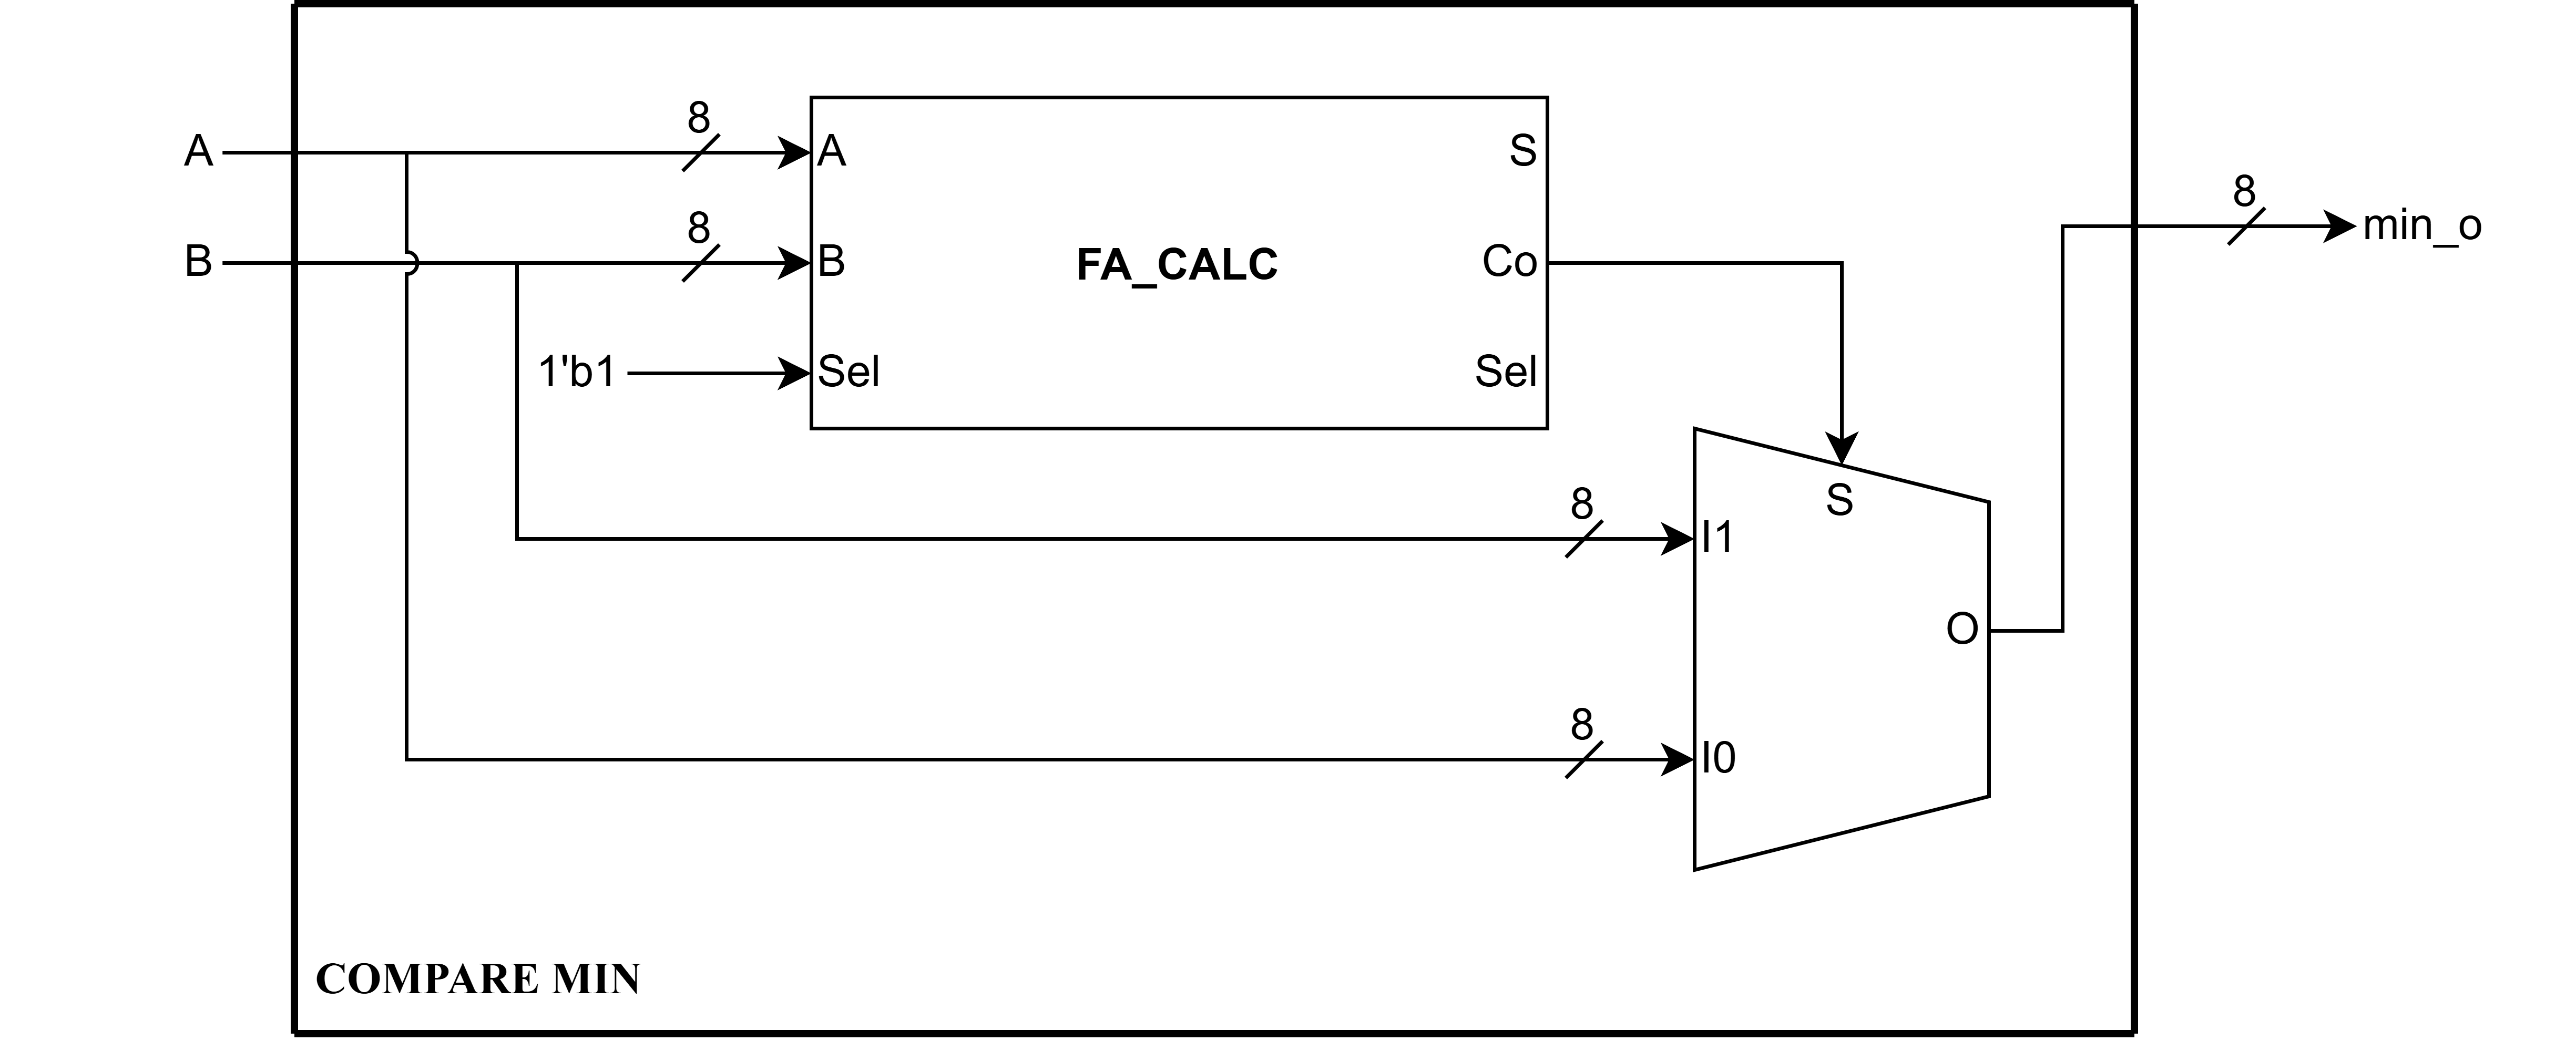
\includegraphics[width=0.7\textwidth]{./images/LDP_DECODER-ABS.drawio (3).png}
    \caption{Kiến trúc phần tử con Comp min}
\end{figure}

\begin{figure}[h!]
        \centering
    \includegraphics[width=0.9\textwidth]{./images/LDP_DECODER-ABS.drawio (4).png}
    \caption{Kiến trúc Khối Compare tree}
\end{figure}

\textbf{Khối khôi phục dấu và tạo bản tin CTV (\texttt{sign\_insertion}):}
    Bước cuối cùng của chuỗi xử lý là kết hợp bít dấu mới và biên độ để tạo thành bản tin hoàn chỉnh dạng bù 2. Bít dấu cho bản tin $CTV_i$ trên nhánh thứ $i$ được cập nhật bằng cách XOR bít dấu toàn cục với bít dấu ban đầu của chính nó. Sau đó, dựa vào bít dấu mới này, dữ liệu lại được đưa qua khối \texttt{fa\_calc} để chuyển đổi từ biên độ thuần túy sang số có dấu bù 2:
    \begin{align}
        Sign_{CTV_i} &= sign\_total \oplus sign\_o_i \nonumber \\
        CTV_i &= \begin{cases}
            y_i & \text{nếu } Sign_{CTV_i} = 0 \\
            \sim y_i + 1 & \text{nếu } Sign_{CTV_i} = 1
        \end{cases}
    \end{align}

Nhìn chung, bằng cách sử dụng chung một mô-đun toán học lõi (\texttt{fa\_calc}) cho cả quá trình lấy trị tuyệt đối, so sánh trừ, và khôi phục dấu, kiến trúc này giúp tiết kiệm đáng kể số lượng cell logic trên FPGA. Cấu trúc tổ hợp hoàn toàn (combinational logic) từ ngõ vào $VTC$ đến ngõ ra $CTV$ cho phép trễ lan truyền được tối ưu, phù hợp cho các thiết kế giải mã yêu cầu thông lượng cao.

\begin{figure}[h!]
        \centering
    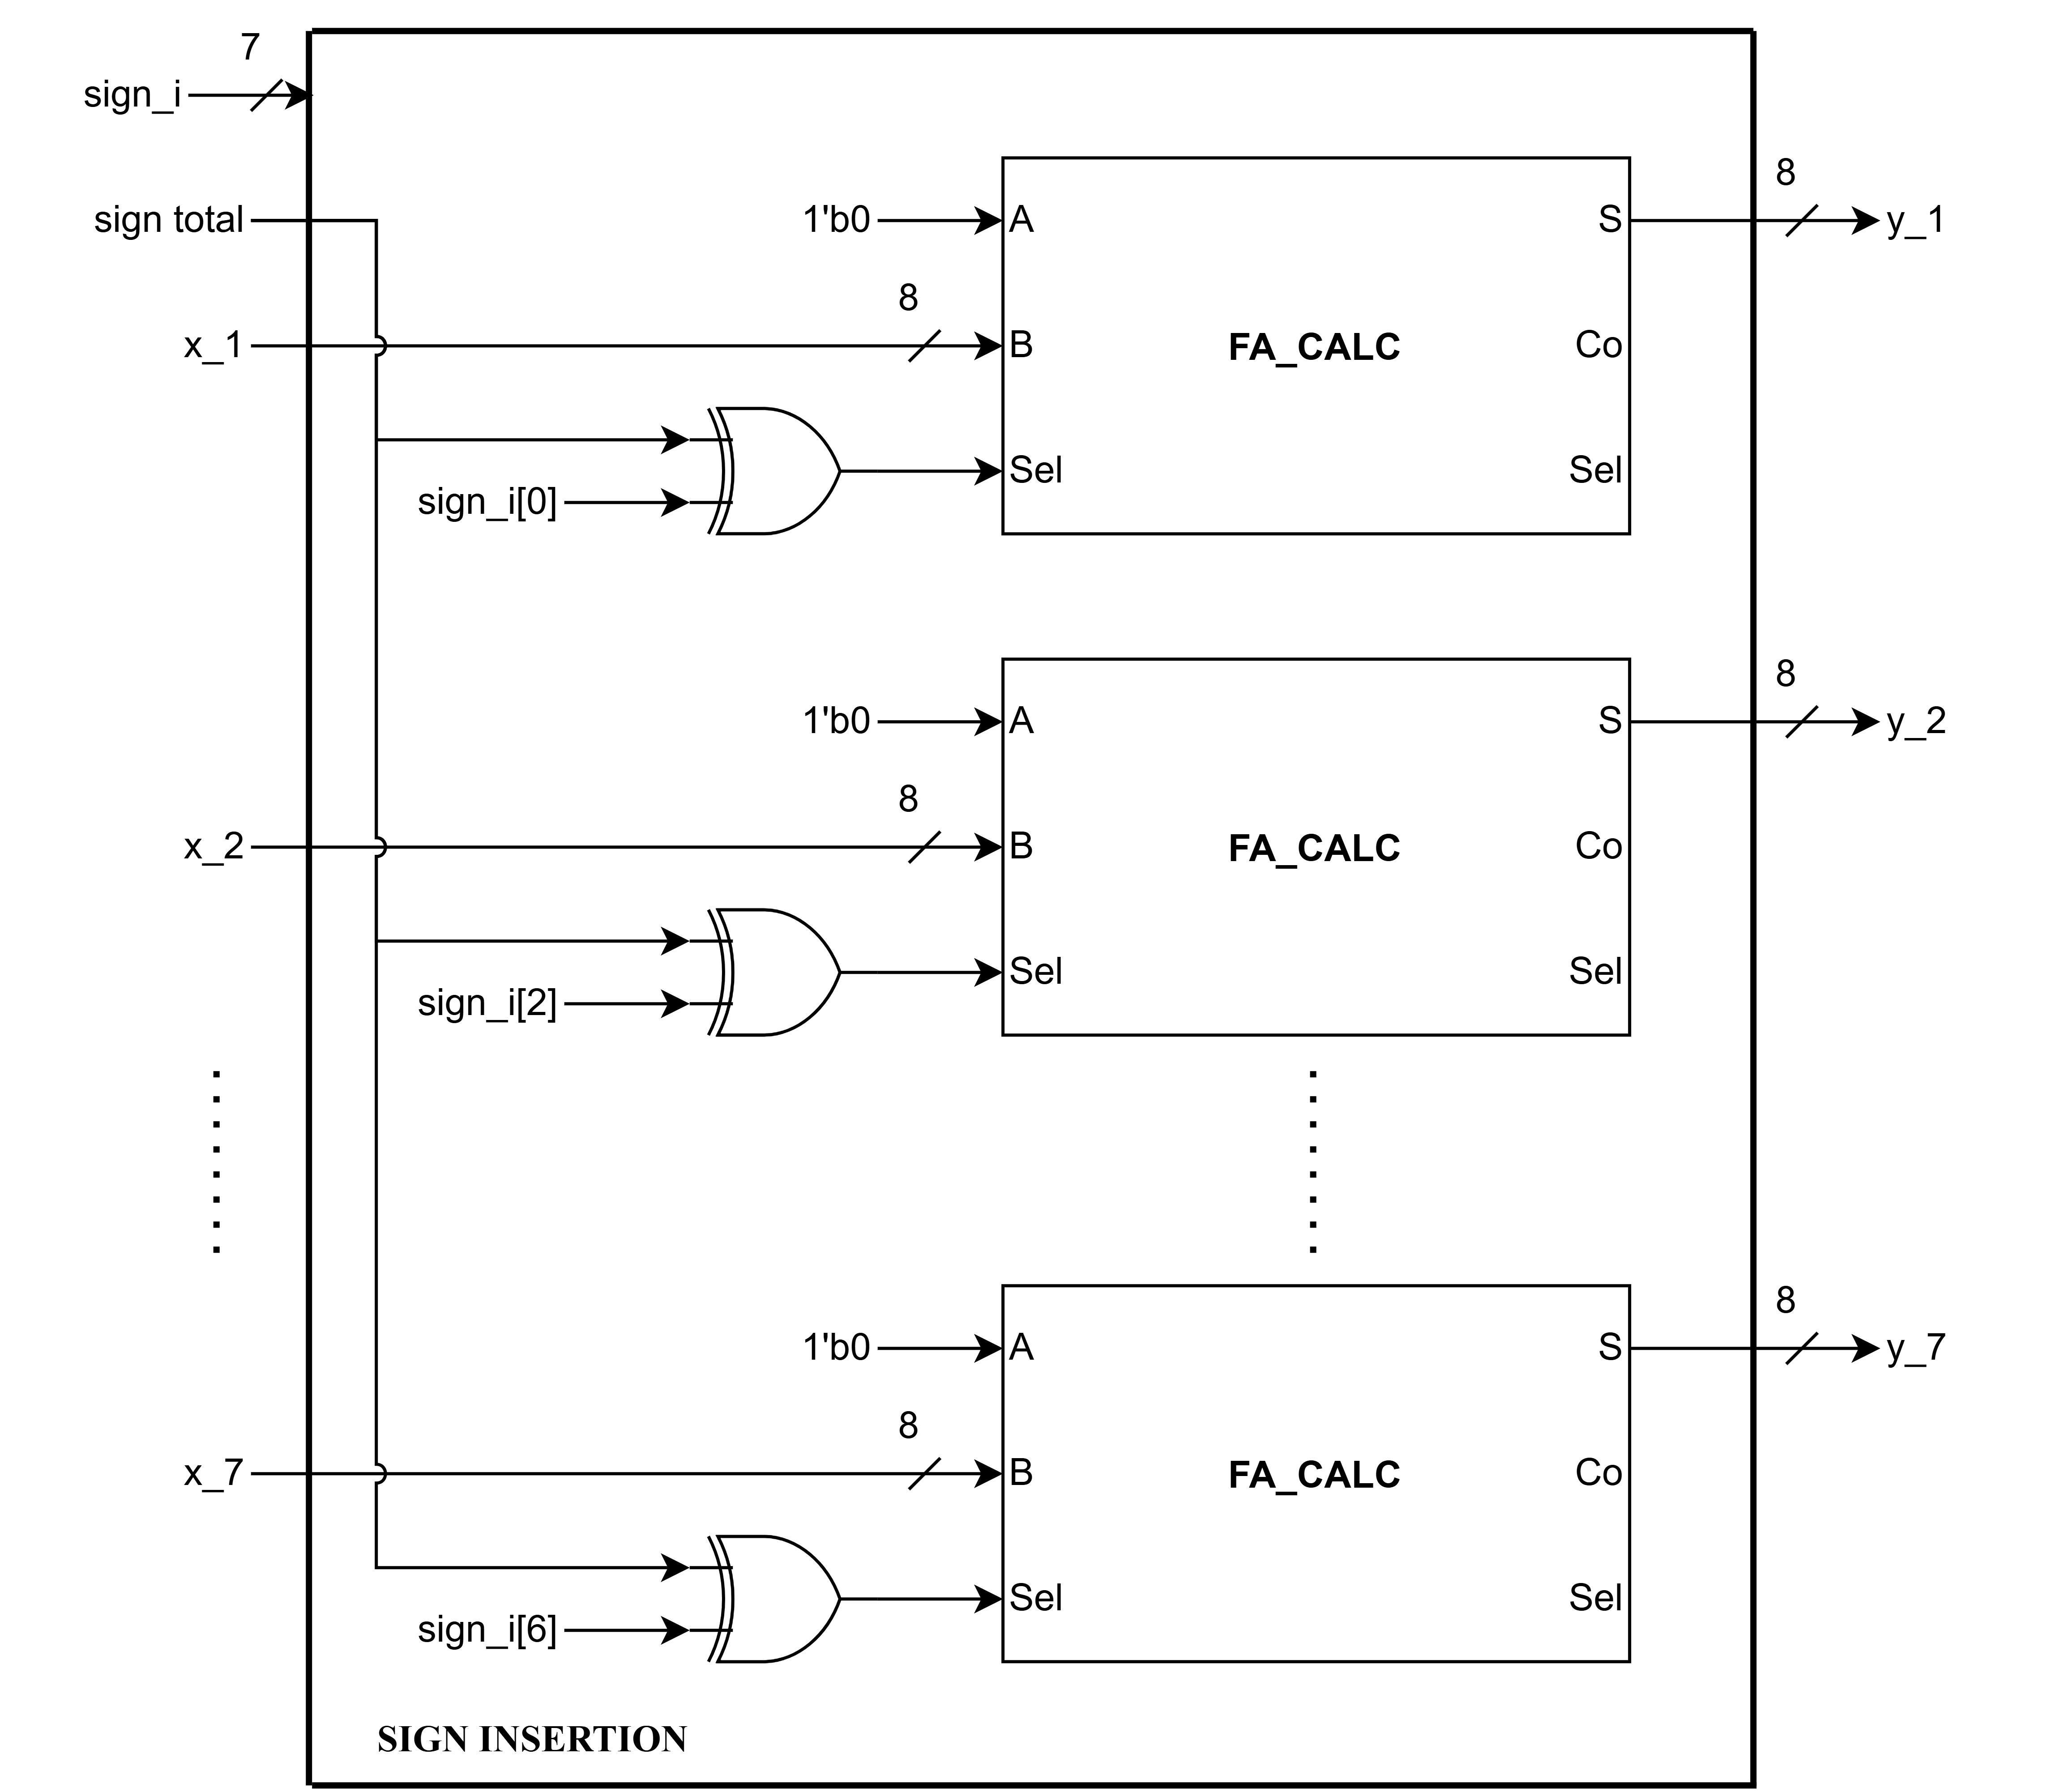
\includegraphics[width=0.9\textwidth]{./images/LDP_DECODER-SIGN.INSERT.drawio.png}
    \caption{Kiến trúc Khối Sign Insertion}
\end{figure}
\newpage
\section{Khối CTV \& APP Calculation}
\begin{figure}[h!]
        \centering
    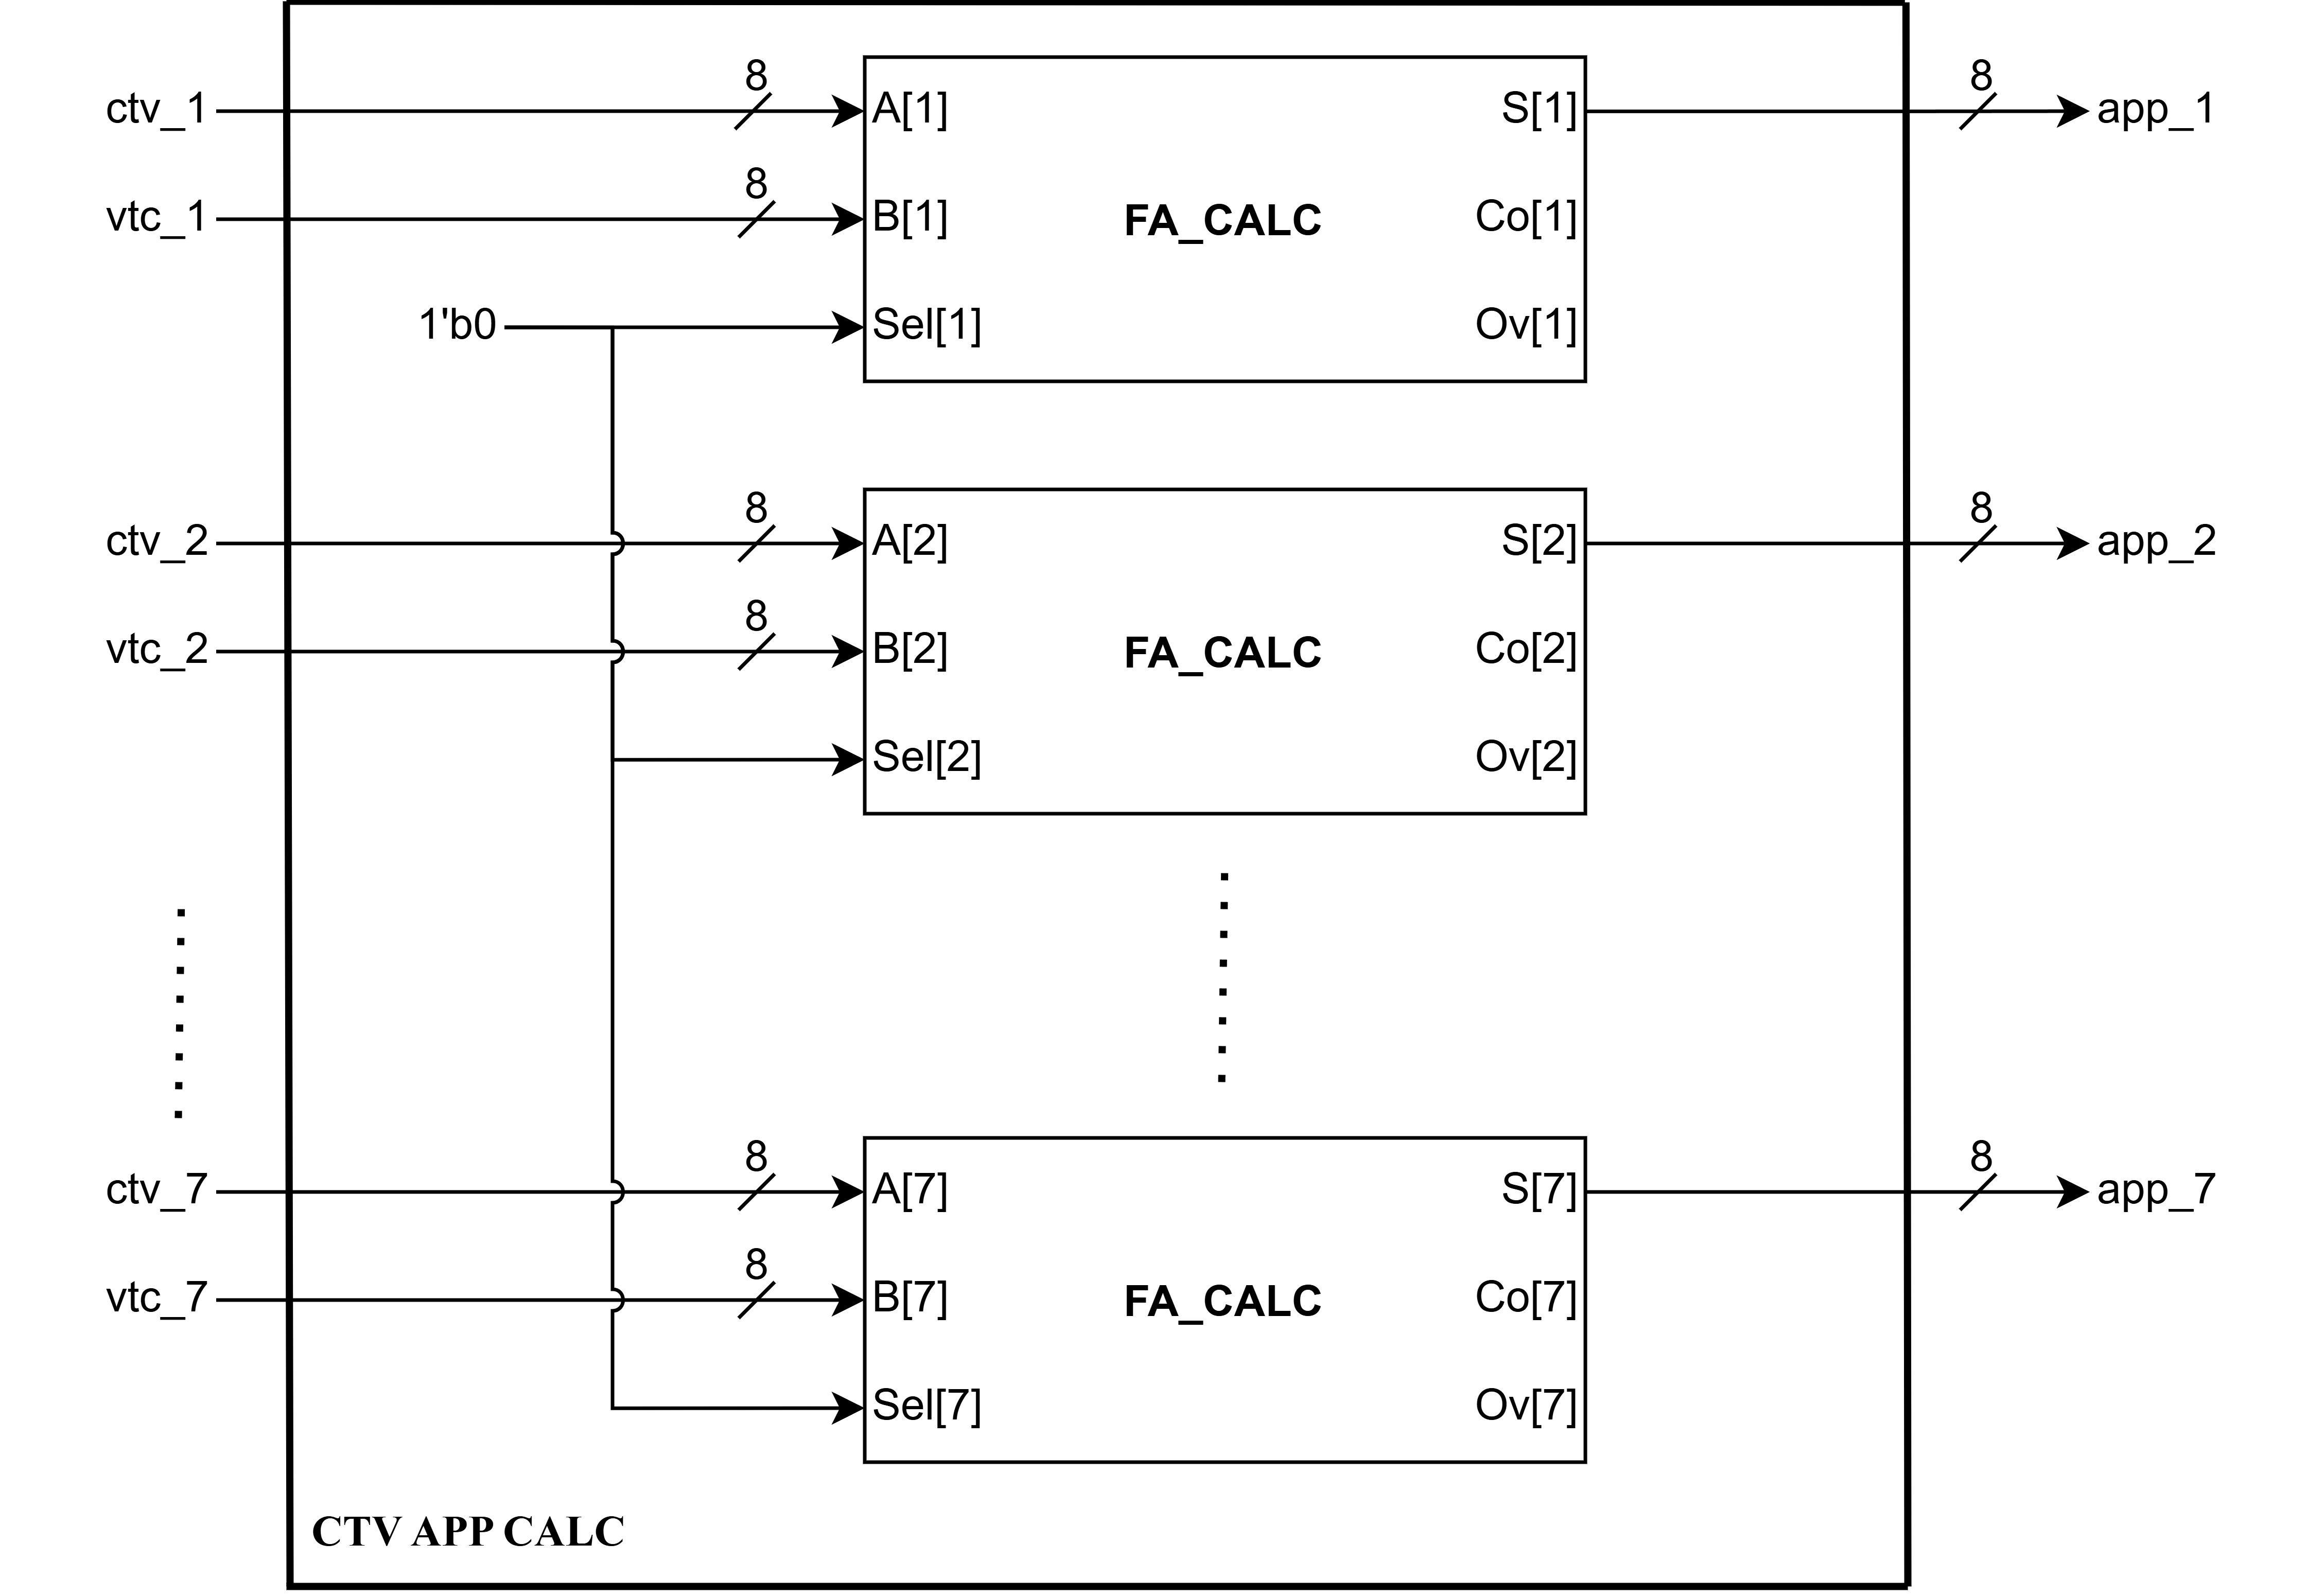
\includegraphics[width=0.85\textwidth]{./images/LDP_DECODER-CTV APP CALC.drawio.png}
    \caption{Kiến trúc Khối CTV APP CALC}
\end{figure}

Khối CTV \& APP Calculation có nhiệm vụ kết hợp các giá trị \textit{VTC} và \textit{CTV} tương ứng để tạo ra các giá trị \textit{APP} ở đầu ra. Trong thiết kế, bảy cặp dữ liệu $\left(VTC_i,CTV_i\right)$ được xử lý song song, với $i\in\{1,\ldots,7\}$. Mỗi phép tính được thực hiện bằng một module \texttt{fa\_calc} nhằm tận dụng cấu trúc bộ cộng dựa trên Full Adder đã được sử dụng trong các khối tính toán trước đó.

\textbf{Cấu trúc:} Khối \texttt{ctv\_app\_calc} gồm 7 instance \texttt{fa\_calc} hoạt động song song. Với mỗi nhánh $i$, hai dữ liệu $VTC_i$ và $CTV_i$ được đưa vào hai đầu vào của \texttt{fa\_calc}. Tín hiệu \texttt{Sel} được đặt bằng $0$ để lựa chọn phép cộng. Kết quả được đưa trực tiếp đến ngõ ra $APP_i$.

\textbf{Nguyên lý hoạt động:} Với mỗi nhánh $i$, khối thực hiện phép cộng giữa giá trị VTC và CTV tương ứng:

\begin{equation}
    APP_i = VTC_i + CTV_i,
    \qquad i\in\{1,\ldots,7\}.
\end{equation}

Do đó, toàn bộ bảy giá trị APP được tính độc lập theo:

\begin{align}
    APP_1 &= VTC_1 + CTV_1, &
    APP_2 &= VTC_2 + CTV_2, \nonumber\\
    APP_3 &= VTC_3 + CTV_3, &
    APP_4 &= VTC_4 + CTV_4, \nonumber\\
    APP_5 &= VTC_5 + CTV_5, &
    APP_6 &= VTC_6 + CTV_6, \nonumber\\
    APP_7 &= VTC_7 + CTV_7. &&
\end{align}

Các phép tính được thực hiện song song nhờ bảy module \texttt{fa\_calc}, giúp tạo đồng thời các giá trị APP tương ứng.

% \section{Hardware Design}

% In this section, cover the hardware design aspects, including:
% \begin{itemize}
%     \item The choice of FPGA platform.
%     \item Design specifications and requirements.
%     \item The hardware architecture and components.
%     \item The design process, including schematic and layout considerations.
%     \item Any simulations or analyses performed to validate the design.
% \end{itemize}

% \section{Software Design}
% Discuss the software design that complements the hardware implementation. Include:
% \begin{itemize}
%     \item The development environment and tools used.
%     \item The integration between hardware and software.
%     \item Firmware or drivers developed for the FPGA.
%     \item Software algorithms and their implementation.
%     \item Testing and debugging procedures.
% \end{itemize}

% %%%%%%%%%%%%%%%%%%%%

\chapter{Thực hiện phần mềm và mô phỏng}
% \section{Khối Full Adder}
% Bao gồm 2 module, trong đó module chính là fa\_calc đảm nhận việc cộng trừ 8 bit có điều khiển sử dụng module con là fa. Chức năng cơ bản chính của fa\_calc được xây dựng bằng cách ghép 8 khối fa ở trên (fa0 đến fa7). Tính năng đặc biệt thông qua tín hiệu Sel:
% \begin{itemize}
%     \item Khi Sel = 0 (Phép cộng): Tín hiệu vào $b$ của các khối fa giữ nguyên ($B[i] \oplus 0 = B[i]$). Ngõ vào chuyển mạch ban đầu $ci$ của khối fa0 bằng $0$.Khối thực hiện phép tính: $S = A + B + 0$.
%     \item Khi Sel = 1 (Phép trừ - Bù 2): Tín hiệu vào $b$ bị đảo trạng thái ($B[i] \oplus 1 = \overline{B[i]}$). Ngõ vào $ci$ của khối fa0 được gán bằng $1$.Theo nguyên lý bù 2, việc đảo bit và cộng thêm 1 tương đương với phép toán: $A + \overline{B} + 1 = A - B$.
%     \item Các ngõ ra mở rộng: Co (Carry out): Cờ nhớ tràn ở bit thứ 8 (temp[7]). Ov (Overflow): Cờ báo tràn số có dấu (signed overflow), được tính bằng phép XOR giữa cờ nhớ của bit thứ 7 và bit thứ 6 (temp[7] \^ temp[6]).
% \end{itemize}

% Sau đây là các dạng sóng thể hiện cách hoạt động của 2 khối:
% \begin{figure}[h!]
%     \centering
%     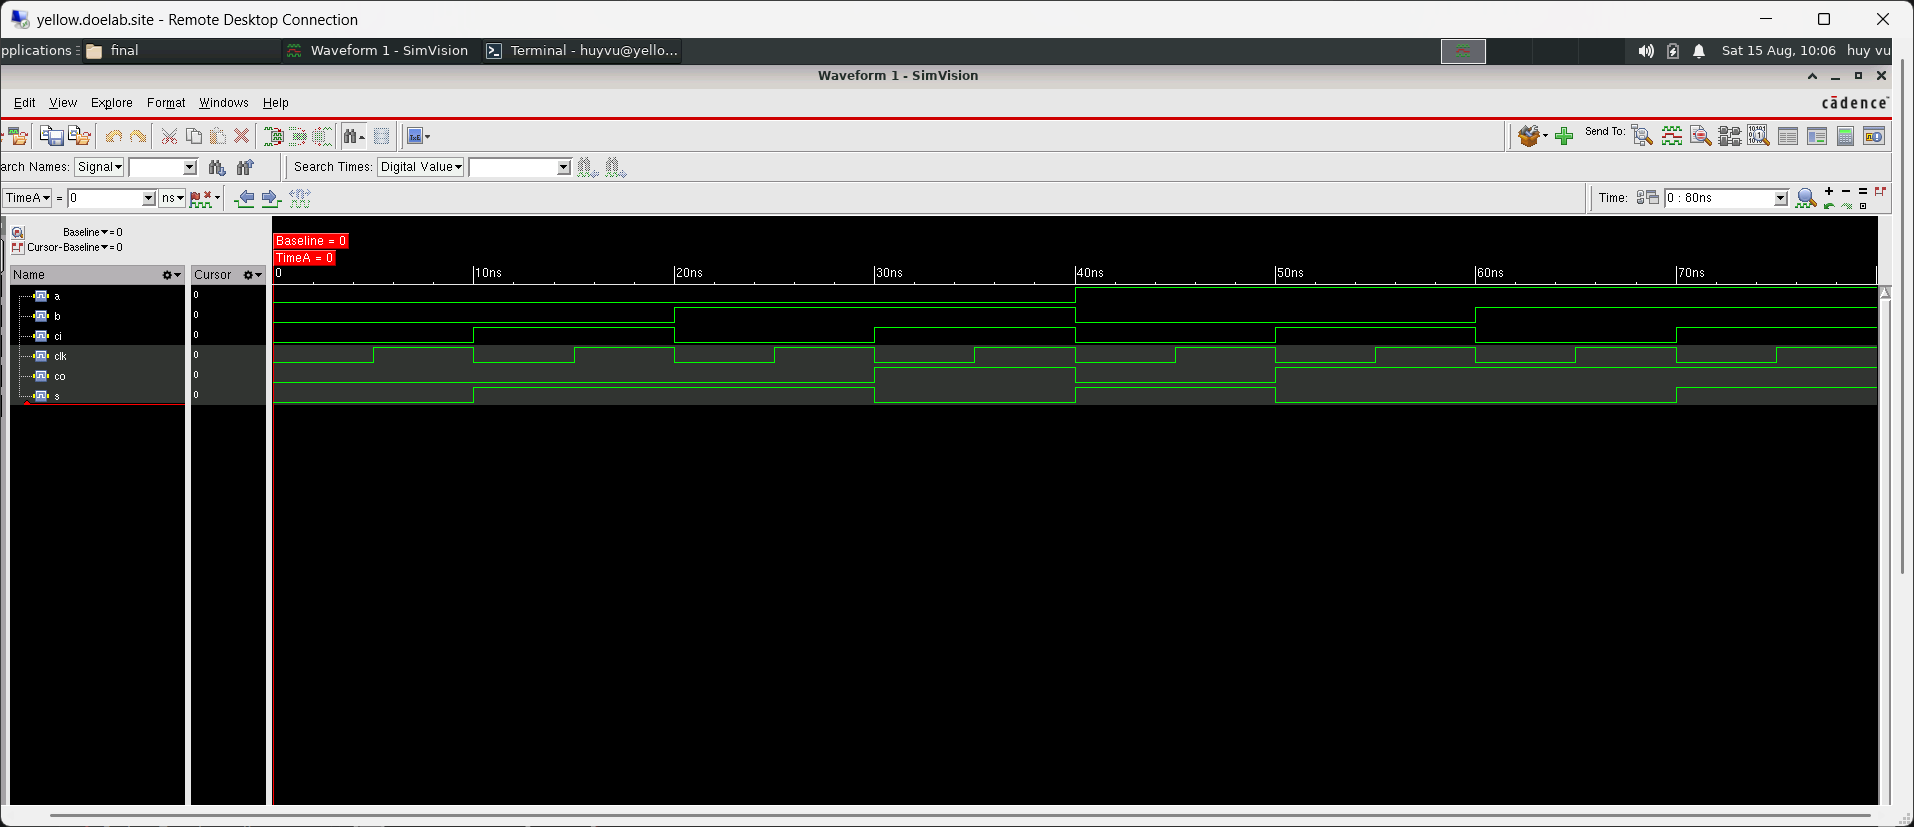
\includegraphics[width=\textwidth]{./images/fa_waveform.png}
%     \caption{Dạng sóng của khối fa}
% \end{figure}

% Nhận xét: Khối fa hoạt động hoàn toàn theo nguyên lý mạch logic tổ hợp thuần túy. Ngay khi các tín hiệu ngõ vào a, b, hoặc ci thay đổi trạng thái, các ngõ ra s và co sẽ phản hồi và cập nhật giá trị mới gần như tức thời (chỉ chịu một độ trễ lan truyền nhỏ của cổng logic), hoàn toàn không phụ thuộc vào xung nhịp clk.
% \newpage
% \begin{figure}[h!]
%     \centering
%     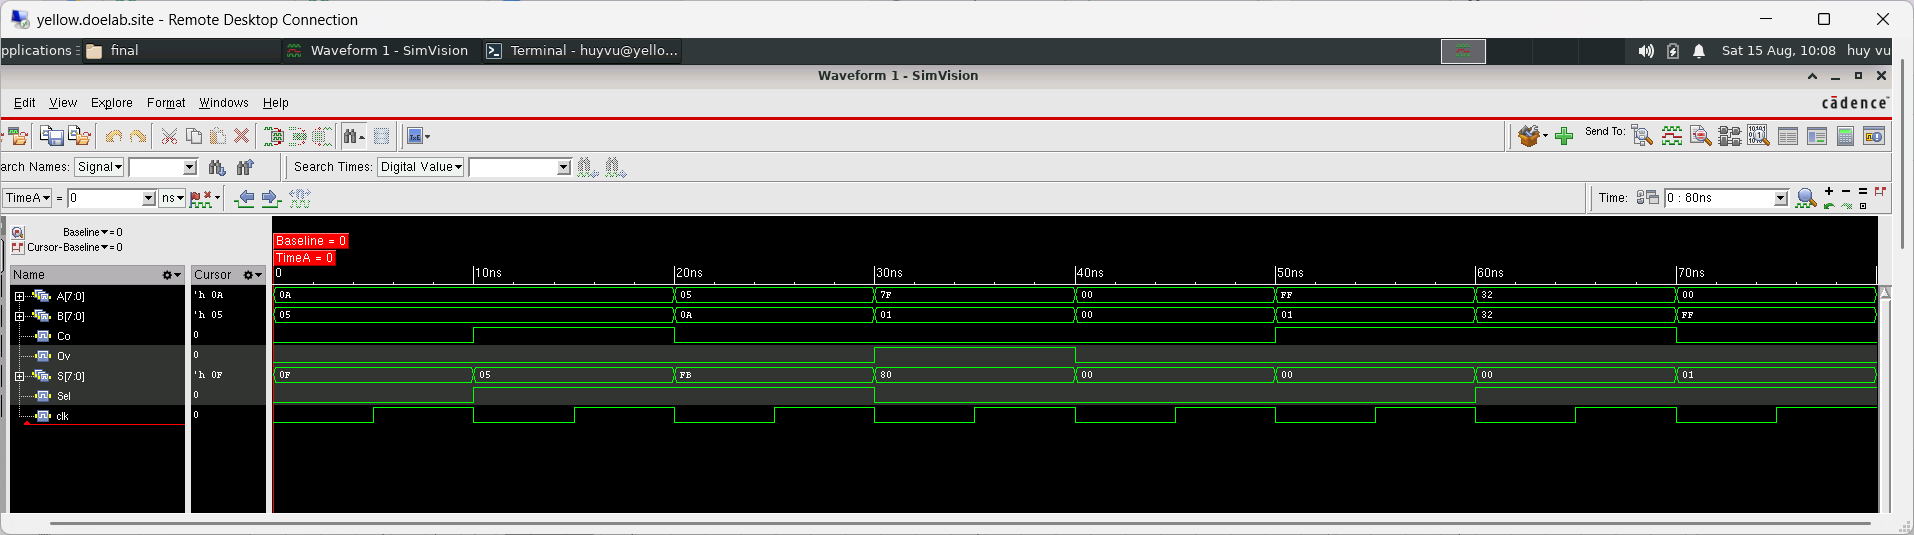
\includegraphics[width=\textwidth]{./images/fa_calc.waveform.png}
%     \caption{Dạng sóng của khối fa}
% \end{figure}

% Nhận xét: Khối fa\_calc thực hiện các phép toán số học 8-bit bằng cách ghép nối tuần tự 8 khối fa (fa0 đến fa7). Các ngõ vào A[7:0] và B[7:0] được xử lý đồng thời qua mạng lưới truyền nhớ lan truyền.
% \begin{itemize}
%     \item Trường hợp 1 ($0\text{ns} - 18\text{ns}$): $A = 0\text{x0A}$ (10), $B = 0\text{x05}$ (5), $\text{Sel} = 0$ (phép cộng). Kết quả: $S = 0\text{x0F}$ (15), $\text{Co} = 0, \text{Ov} = 0$ $\rightarrow$ Chính xác.
%     \item Trường hợp 2 ($18\text{ns} - 27\text{ns}$): Đảo vị trí $A = 0\text{x05}$, $B = 0\text{x0A}$, $\text{Sel} = 0$. Kết quả: $S = 0\text{x0F}$ (15), $\text{Co} = 0, \text{Ov} = 0$ $\rightarrow$ Tính giao hoán của phép cộng hoạt động đúng.
%     \item Trường hợp 3 ($27\text{ns} - 36\text{ns}$): $A = 0\text{x7F}$ (+127), $B = 0\text{x01}$ (+1), $\text{Sel} = 0$. Kết quả: $S = 0\text{x80}$ (-128 ở dạng có dấu), $\text{Co} = 0$, và Cờ tràn số có dấu Ov bật lên mức 1. Điều này hoàn toàn chính xác vì tổng vượt quá giới hạn dương của số có dấu 8-bit (+127), kích hoạt mạch phát hiện tràn (temp[7] $\wedge$ temp[6]).
%     \item Trường hợp 4 ($45\text{ns} - 54\text{ns}$): $A = 0\text{xFF}$ (255), $B = 0\text{x01}$ (1), $\text{Sel} = 0$. Kết quả: $S = 0\text{x00}$ và Cờ nhớ không dấu Co bật lên mức 1 do kết quả vượt quá 8-bit ($\text{255} + \text{1} = \text{256}$).
% \end{itemize}

% Thời gian đáp ứng: Tương tự khối fa, toàn bộ chuỗi 8-bit phản hồi tức thời theo sự thay đổi của bus dữ liệu ngõ vào mà không cần chờ chu kỳ xung nhịp
% \section{Khối ABS}

\section{Khối BRAM APP}
Bước đầu ta sẽ khảo sát dạng sóng waveform của thiết kế khối này.
\begin{figure}[h!]
    \centering
    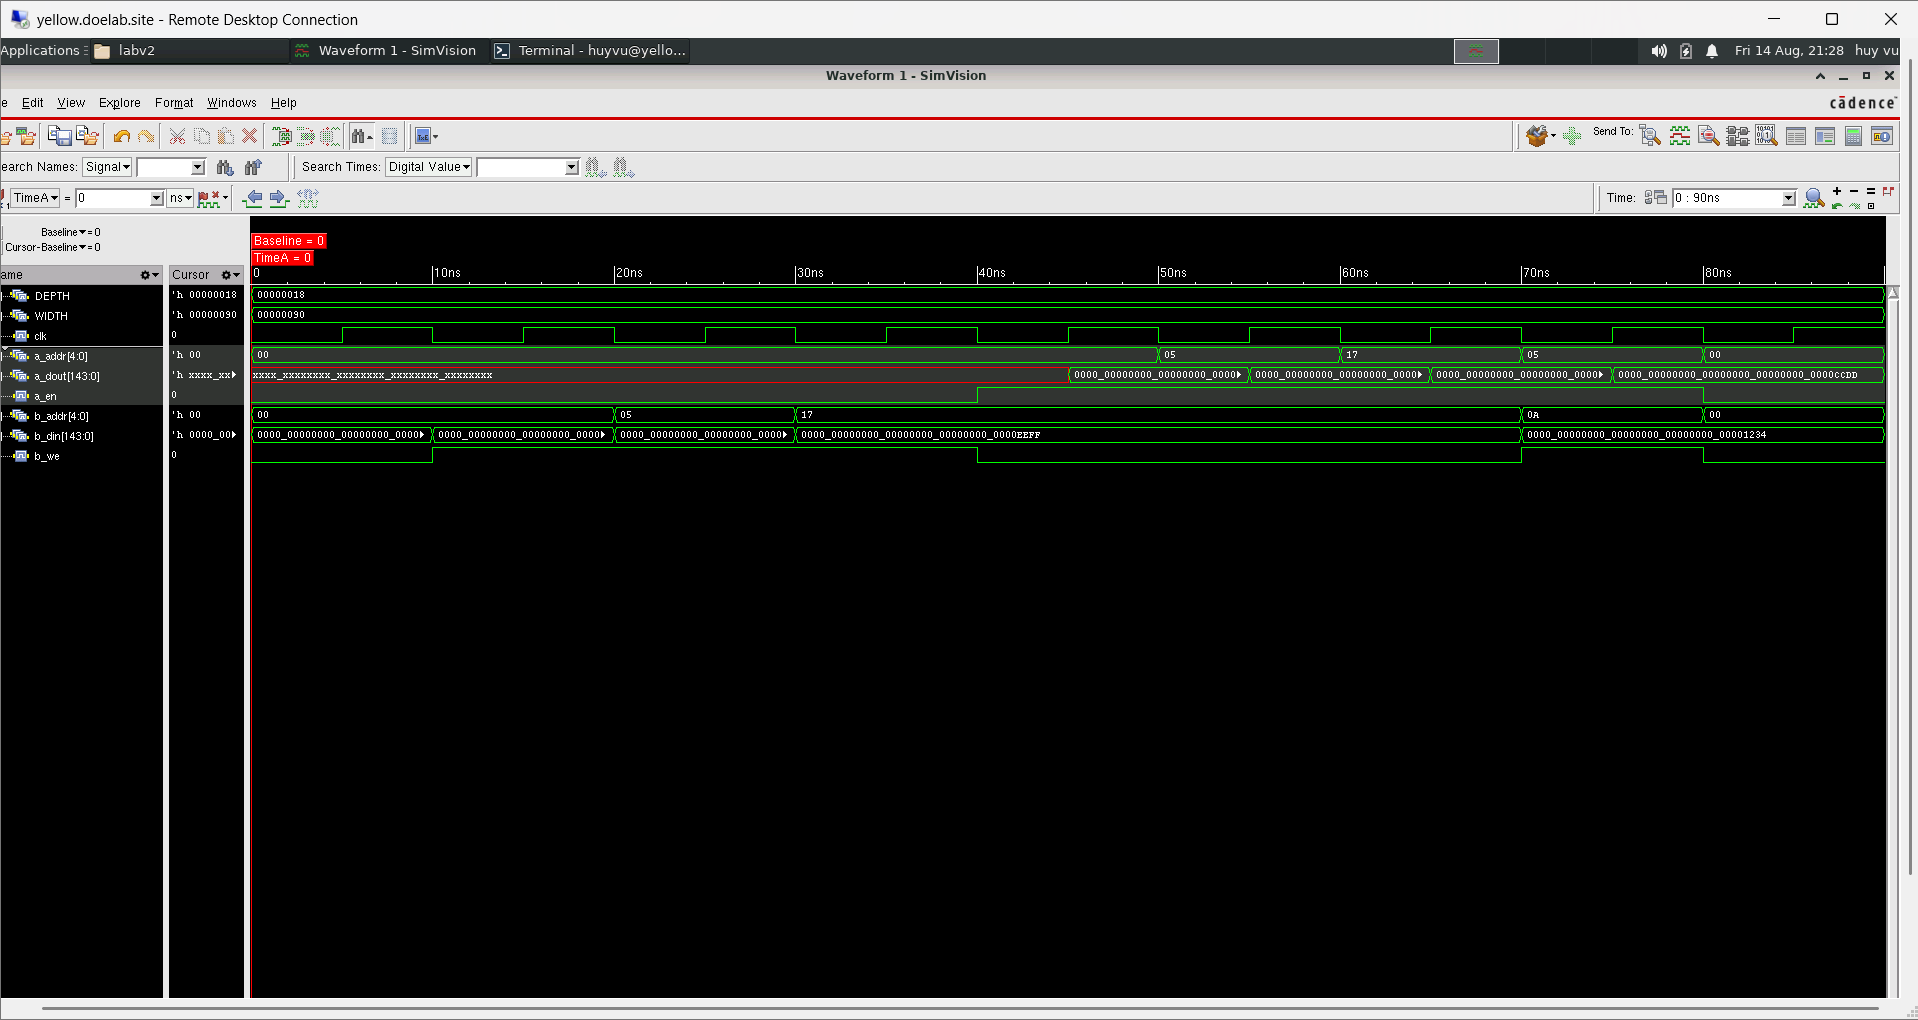
\includegraphics[width=\textwidth]{./images/bram_app_waveform.png}
    \caption{Dạng sóng của khối BRAM APP}
\end{figure}

Quan sát cửa sổ mô phỏng SimVision, ta có thể theo dõi rõ ràng mối quan hệ giữa các tín hiệu điều khiển và dữ liệu qua từng clk. Khởi tạo khối BRAM với tham số K trong trường hợp này là DEPTH = 24 và độ rộng bus dữ liệu WIDTH = 144 bits.
\begin{itemize}
    \item \textit{Hoạt động của Cổng B (Ghi dữ liệu - Write Port)}. 
    \begin{itemize}
        \item Tín hiệu điều khiển: Gồm b\_we (Write Enable), b\_addr[4:0] (Địa chỉ ghi), và b\_din[143:0] (Dữ liệu ngõ vào).
        \item Khi b\_we chuyển lên mức cao (logic 1), tại mỗi sườn dương của xung nhịp clk, dữ liệu xuất hiện trên bus b\_din sẽ được ghi vào mảng bộ nhớ mem tại vị trí địa chỉ tương ứng của b\_addr. Các giá trị dữ liệu như 0000\_00000000 \_00000000\_00000000\_0000EEFF, 0000
        \_00000000\_00000000 \_00000000\\ \_000001234,... được ghi lần lượt vào các địa chỉ 00, 05, 17, 0A khi b\_we được kích hoạt. 
    \end{itemize}
    \item \textit{Hoạt động của Cổng A (Đọc dữ liệu - Read Port)}.
    \begin{itemize}
        \item Tín hiệu điều khiển: Gồm a\_en (Read Enable), a\_addr[4:0] (Địa chỉ đọc), và a\_dout[143:0] (Dữ liệu ngõ ra).
        \item Ban đầu, khi chưa có lệnh đọc, ngõ ra a\_dout ở trạng thái không xác định (xxxx...). Khi a\_en được bật lên mức cao, tại sườn dương tiếp theo của clk, bộ nhớ thực hiện đọc dữ liệu tại ô nhớ có địa chỉ a\_addr và đưa ra ngõ ra a\_dout. Do sử dụng thanh ghi đồng bộ (always\_ff), dữ liệu ngõ ra a\_dout có độ trễ 1 chu kỳ xung nhịp so với thời điểm địa chỉ a\_addr và enable a\_en được thiết lập. Các giá trị lưu trữ (như 0000\_00000000\_00000000\_00000000\_0000ccdd) được xuất ra chính xác theo đúng yêu cầu địa chỉ đọc (00, 05, 17,...).
    \end{itemize}
     
\end{itemize}

Tiếp đến, ta tiến hành đo đạc các thông số thời gian, diện tích và công suất của khối.
\begin{table}[H]
\centering
\resizebox{0.8\textwidth}{!}{
\begin{tabular}{|l|c|c|}
\hline
\textbf{Library Name} 
& \textbf{Total Area} 
& \textbf{Total Power} \\
\hline

fast\_vdd1v0\_basicCells\_hvt & 31678.434 & 4.70108e-03 \\ \hline
fast\_vdd1v2\_basicCells\_hvt & 31678.571 & 6.95173e-03 \\ \hline
slow\_vdd1v0\_basicCells\_hvt & 32070.024 & 3.07382e-03 \\ \hline
slow\_vdd1v2\_basicCells\_hvt & 31725.972 & 4.48042e-03 \\ \hline
fast\_vdd1v0\_basicCells\_lvt & 34346.855 & 6.30073e-03 \\ \hline
fast\_vdd1v2\_basicCells\_lvt & 34313.202 & 9.34758e-03 \\ \hline
slow\_vdd1v0\_basicCells\_lvt & 31684.932 & 3.43799e-03 \\ \hline
slow\_vdd1v2\_basicCells\_lvt & 31688.010 & 5.09793e-03 \\ \hline

\end{tabular}
}
\caption{Tổng hợp thông số Diện tích và Công suất của khối BRAM APP qua các process corners.}
\end{table}

\begin{table}[h]
\centering
\resizebox{\textwidth}{!}{%
\begin{tabular}{@{}clp{8cm}cc@{}}
\toprule
\textbf{STT} & \textbf{Góc PVT} & \textbf{Đường đi tín hiệu (Critical Path)} & \textbf{Độ trễ (ps)} & \textbf{Thời gian dư (ps)} \\ \midrule
1 & fast\_1v2\_lvt & a\_en $\rightarrow$ INVX2LVT $\rightarrow$ NOR3X1LVT $\rightarrow$ AND3X2LVT $\rightarrow$ AOI22XLLVT $\rightarrow$ NAND4XLLVT $\rightarrow$ OR3XLLVT & 649 & 812 \\
2 & fast\_1v0\_lvt & a\_en $\rightarrow$ INVX2LVT $\rightarrow$ NOR3X1LVT $\rightarrow$ AND3X2LVT $\rightarrow$ AOI22XLLVT $\rightarrow$ NAND4XLLVT $\rightarrow$ OR3XLLVT & 893 & 539 \\
3 & fast\_1v2\_hvt & a\_addr[2] $\rightarrow$ INVX1LVT $\rightarrow$ OAI22XLLVT $\rightarrow$ AOI221X1LVT $\rightarrow$ AOI221X1LVT $\rightarrow$ OAI22XLLVT $\rightarrow$ MX2XLLVT & 303 & 1177 \\
4 & fast\_1v0\_hvt & a\_addr[1] $\rightarrow$ INVX2HVT $\rightarrow$ BUFX2HVT $\rightarrow$ INVX1HVT $\rightarrow$ OAI22X1LVT $\rightarrow$ AOI22XLLVT $\rightarrow$ MX2XLLVT & 477 & 997 \\
5 & slow\_1v2\_lvt & a\_en $\rightarrow$ INVX3HVT $\rightarrow$ NOR3X1HVT $\rightarrow$ AND3X4HVT $\rightarrow$ AOI22XLHVT $\rightarrow$ NAND4XLHVT $\rightarrow$ OR3XLHVT & 964 & 459 \\
6 & slow\_1v0\_lvt & a\_en $\rightarrow$ CLKINVX20HVT $\rightarrow$ NOR3X6HVT $\rightarrow$ CLKAND2X2HVT $\rightarrow$ AND2X8HVT $\rightarrow$ INVX2HVT $\rightarrow$ AOI211X1HVT $\rightarrow$ OR4X1HVT & 1301 & 2 \\
7 & slow\_1v2\_hvt & a\_en $\rightarrow$ INVX2HVT $\rightarrow$ NOR2X1HVT $\rightarrow$ AND2X1HVT $\rightarrow$ CLKAND2X2HVT $\rightarrow$ AOI22X1HVT $\rightarrow$ NAND4XLHVT $\rightarrow$ OR3XLHVT & 941 & 946 \\
8 & slow\_1v0\_hvt & a\_en $\rightarrow$ INVX2HVT $\rightarrow$ NOR2XLHVT $\rightarrow$ AND2X1HVT $\rightarrow$ AND2X2HVT $\rightarrow$ AOI222X1HVT $\rightarrow$ NAND4XLHVT $\rightarrow$ OR3XLHVT & 1025 & 854 \\ \bottomrule
\end{tabular}%
}
\caption{Thống kê độ trễ các góc phân tích (PVT corners) cho khối bram\_app.}
\end{table}

Đặc tính thời gian:
\begin{itemize}
    \item Ảnh hưởng của góc PVT: Thời gian trễ của đường truyền tới các tín hiệu ngõ ra (a\_dout\_reg) chịu ảnh hưởng mạnh mẽ bởi sự thay đổi của điện áp nguồn và ngưỡng chuyển mạch của transistor. Ở các góc slow, độ trễ tăng đáng kể do điện áp giảm xuống $1.0\text{V}$ và đặc tính dẫn của transistor suy giảm.
    \item Điểm tới hạn: Góc phân tích slow\_1v0\_lvt là góc ảnh hưởng nhất đối với toàn bộ thiết kế. Đường đi tín hiệu dài nhất đạt độ trễ lên đến 1301 ps với thời gian dư (Slack) chỉ còn vỏn vẹn 2 ps. Điều này cho thấy mạch hoạt động cực kỳ sát nút với giới hạn setup time, dễ dẫn đến vi phạm timing nếu có dao động nhỏ về nhiệt độ hoặc sụt áp trên thực tế.
    \item Ngược lại ở góc nhanh: Ở các góc nhanh (fast\_1v2\_hvt hoặc fast\_1v2\_lvt), độ trễ giảm mạnh (chỉ từ 303 ps đến 649 ps) và thời gian dư dồi dào (Slack lên tới trên 1100 ps), đảm bảo biên an toàn lớn cho tần số hoạt động cao.
\end{itemize}

Diện tích và công suất: 
\begin{itemize}
    \item Đặc tính Thư viện Cell (HVT và LVT):Các thiết kế sử dụng thư viện LVT có tốc độ chuyển mạch nhanh hơn nhưng đổi lại làm tăng tổng diện tích mạch (lên đến khoảng $34,346$ đơn vị) do yêu cầu kích thước transistor hoặc đệm lót tối ưu. Ngược lại, các góc sử dụng thư viện HVT giúp tối ưu diện tích tốt hơn (dao động quanh mức $31,678$ đến $32,070$ đơn vị) và kìm hãm dòng rò hiệu quả.
    \item Ảnh hưởng của Điện áp nguồn ($V_{DD}$):Khi nâng điện áp từ $1.0\text{V}$ lên $1.2\text{V}$, công suất tiêu thụ tăng lên rõ rệt do thành phần công suất động ($P_{dynamic} \propto C \cdot V^2 \cdot f$) tăng theo bình phương điện áp. Ví dụ, ở nhóm góc fast\_vdd1v2\_lvt, công suất đạt đỉnh lên tới khoảng $9.35 \times 10^{-3}\text{ W}$.
    \item Ngược lại, ở các góc hoạt động ở mức $1.0\text{V}$ kết hợp với cell HVT (slow\_vdd1v0\_ basicCells\_hvt), công suất tiêu thụ được hạ mức tối thiểu xuống còn khoảng $3.07 \times 10^{-3}\text{ W}$, giúp tiết kiệm năng lượng đáng kể cho hệ thống.
\end{itemize}
\section{Khối BRAM CTV}
Bước đầu ta sẽ khảo sát dạng sóng waveform của thiết kế khối này.
\begin{figure}[h!]
    \centering
    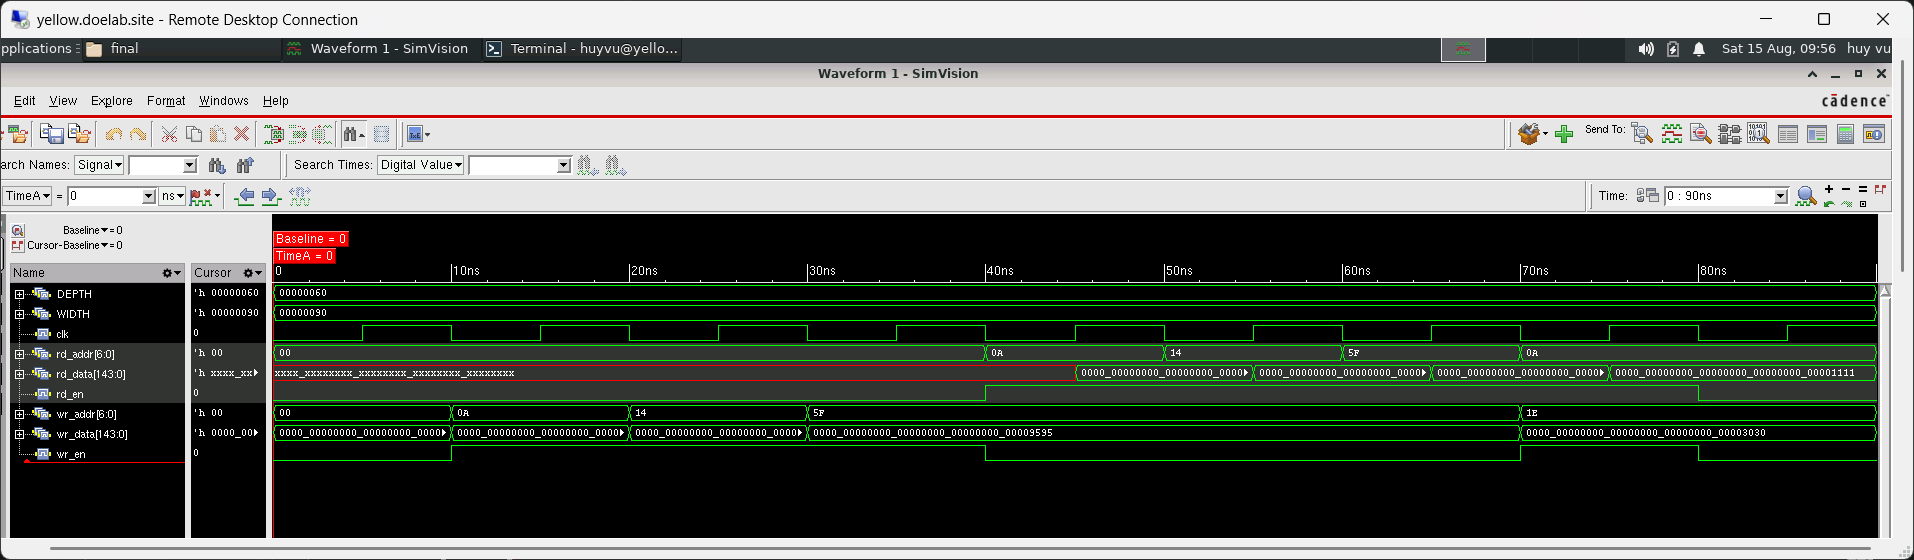
\includegraphics[width=\textwidth]{./images/bram_ctv_waveform.png}
    \caption{Dạng sóng của khối BRAM CTV}
\end{figure}

Khối sử dụng một mảng bộ nhớ mem được điều khiển đồng bộ qua posedge clk. Cả thao tác ghi (wr\_en) và đọc (rd\_en) đều được tích hợp chung trong một khối always\_ff, cho phép thực hiện ghi dữ liệu mới và đọc dữ liệu cũ tại các địa chỉ tương ứng trong cùng một chu kỳ xung nhịp. Dữ liệu đọc ra (rd\_data) được chốt qua thanh ghi (có độ trễ 1 chu kỳ xung nhịp). Khởi tạo khối BRAM với tham số K trong trường hợp này là DEPTH = 24 và độ rộng bus dữ liệu WIDTH = 144 bits. Quan sát cửa sổ mô phỏng SimVision cho khối bram\_ctv, ta thấy rõ sự tương tác giữa các tín hiệu điều khiển và dữ liệu:
\begin{itemize}
    \item \textit{Hoạt động ghi dữ liệu - Write Port}. 
    \begin{itemize}
        \item Tín hiệu điều khiển: Gồm wr\_en (Write Enable), wr\_addr[6:0] (Địa chỉ ghi), và wr\_data[143:0] (Dữ liệu ngõ vào).
        \item Nguyên lý trên sóng tín hiệu: Khi wr\_en lên mức cao (logic 1), tại sườn dương của clk, dữ liệu trên bus wr\_data được ghi vào ô nhớ tại địa chỉ chỉ định bởi wr\_addr. Ví dụ: Các từ dữ liệu lần lượt được ghi vào các địa chỉ 00, 0A, 14, 5F, 1E,... với các giá trị mẫu như 0000\_00000000\_0000\_0000\_0000\_0000\_00009595, 0000\_00000000\_0000\_0000\_0000\_0000\_00000303030,...
    \end{itemize}
    \item \textit{Hoạt động đọc dữ liệu - Read Port}.
    \begin{itemize}
        \item Tín hiệu điều khiển: Gồm rd\_en (Read Enable), rd\_addr[6:0] (Địa chỉ đọc), và rd\_data[143:0] (Dữ liệu ngõ ra).
        \item Nguyên lý trên sóng tín hiệu: Khi rd\_en được bật lên mức cao và rd\_addr được trỏ tới một địa chỉ hợp lệ (ví dụ: 0A, 14, 5F,...), dữ liệu tại ô nhớ đó sẽ được nạp vào thanh ghi đầu ra. Do đặc tính thanh ghi đồng bộ (always\_ff), ngõ ra rd\_data sẽ cập nhật giá trị chính xác sau độ trễ 1 chu kỳ xung nhịp so với thời điểm rd\_addr và rd\_en được xác lập (ví dụ: khi rd\_addr đổi thành 0A, ngõ ra rd\_data đổi sang giá trị tương ứng ở chu kỳ clock tiếp theo).
    \end{itemize}
\end{itemize}

\begin{table}[H]
\centering
\resizebox{0.8\textwidth}{!}{
\begin{tabular}{|l|c|c|}
\hline
\textbf{Library Name} 
& \textbf{Total Area} 
& \textbf{Total Power} \\
\hline

fast\_vdd1v0\_basicCells\_hvt & 31676.040 & 4.50174e-03 \\ \hline
fast\_vdd1v2\_basicCells\_hvt & 31675.698 & 6.64414e-03 \\ \hline
slow\_vdd1v0\_basicCells\_hvt & 32087.192 & 2.95640e-03 \\ \hline
slow\_vdd1v2\_basicCells\_hvt & 31721.184 & 4.28590e-03 \\ \hline
fast\_vdd1v0\_basicCells\_lvt & 34343.435 & 6.01528e-03 \\ \hline
fast\_vdd1v2\_basicCells\_lvt & 34319.358 & 8.85251e-03 \\ \hline
slow\_vdd1v0\_basicCells\_lvt & 31681.170 & 3.28968e-03 \\ \hline
slow\_vdd1v2\_basicCells\_lvt & 31685.274 & 4.87258e-03 \\ \hline

\end{tabular}
}
\caption{Tổng hợp thông số Diện tích và Công suất của khối BRAM CTV qua các process corners.}
\end{table}

\textbf{Phân tích Diện tích (Total Area):}
\begin{itemize}
    \item Diện tích tổng của khối \texttt{bram\_ctv} dao động trong khoảng từ $\sim 31,675.698\,\mu\text{m}^2$ đến $\sim 34,343.435\,\mu\text{m}^2$.
    \item Các cấu hình sử dụng thư viện \textbf{HVT} cho thấy khả năng tối ưu diện tích rất tốt và ổn định, duy trì ở mức khoảng $31,675 - 32,087\,\mu\text{m}^2$. Trong khi đó, các cấu hình sử dụng thư viện \textbf{LVT} có xu hướng chiếm diện tích lớn hơn ở một số góc (đặc biệt tại fast corner lên tới $34,343.435\,\mu\text{m}^2$), do công cụ tổng hợp tự động lựa chọn các cell có kích thước dòng lớn hơn nhằm đáp ứng các ràng buộc về thời gian.
    \item Sự biến động diện tích giữa các góc Fast và Slow trong cùng một nhóm thư viện tế bào là không đáng kể, chứng minh rằng cấu trúc datapath và mảng thanh ghi của khối được ánh xạ phần cứng ổn định.
\end{itemize}

\textbf{Phân tích Công suất tiêu thụ (Total Power):}
\begin{itemize}
    \item Công suất tổng chịu ảnh hưởng mạnh mẽ bởi điện áp nguồn $VDD$ và Process Corner.
    \item Xét về mức điện áp, ở điện áp cao hơn ($1.2\text{V}$), công suất tiêu thụ của mạch luôn lớn hơn đáng kể so với mức $1.0\text{V}$ (ví dụ ở cấu hình fast HVT, công suất tăng từ $4.50174 \times 10^{-3}\text{ mW}$ lên $6.64414 \times 10^{-3}\text{ mW}$).
    \item Xét về góc quá trình, các \textbf{Fast corners} tiêu thụ công suất cao hơn các \textbf{Slow corners} khi ở cùng một mức điện áp (ví dụ: Fast LVT ở $1.2\text{V}$ đạt $8.85251 \times 10^{-3}\text{ mW}$, trong khi Slow LVT ở $1.2\text{V}$ chỉ là $4.87258 \times 10^{-3}\text{ mW}$). Nguyên nhân là do các cell ở góc fast có dòng rò lớn hơn và tốc độ chuyển mạch cao hơn, dẫn đến năng lượng tiêu tán trên chu kỳ xung nhịp tăng lên.
\end{itemize}

Nhìn chung, kết quả phân tích qua các process corners cung cấp cơ sở quan trọng để nhà thiết kế lựa chọn cấu hình thư viện phù hợp với mục tiêu bài toán (ví dụ: sử dụng HVT ở dải điện áp thấp để ưu tiên tiết kiệm năng lượng, hoặc LVT để đảm bảo biên độ thời gian cho các hệ thống xung nhịp cao).

\begin{table}[h]
\centering
\resizebox{\textwidth}{!}{%
\begin{tabular}{@{}clp{8cm}cc@{}}
\toprule
\textbf{STT} & \textbf{Góc PVT} & \textbf{Đường đi tín hiệu (Critical Path)} & \textbf{Độ trễ (ps)} & \textbf{Thời gian dư (ps)} \\ \midrule
1 & fast\_1v0\_hvt & rd\_en $\rightarrow$ INVX2HVT $\rightarrow$ NOR2XLHVT $\rightarrow$ AND2X1HVT $\rightarrow$ AND2X2HVT $\rightarrow$ AOI222X1HVT $\rightarrow$ NAND4XLHVT $\rightarrow$ OR3XLHVT $\rightarrow$ rd\_data\_reg[139]/D & 624 & 854 \\
2 & fast\_1v2\_hvt & rd\_en $\rightarrow$ INVX1HVT $\rightarrow$ NOR2X1HVT $\rightarrow$ AND2X1HVT $\rightarrow$ CLKAND2X2HVT $\rightarrow$ AOI221X1HVT $\rightarrow$ NAND4XLHVT $\rightarrow$ OR3L\_5122/Y $\rightarrow$ rd\_data\_reg[143]/D & 541 & 946 \\
3 & slow\_1v0\_hvt & rd\_addr[3] $\rightarrow$ NOR2X2HVT $\rightarrow$ NAND2X2HVT $\rightarrow$ INVX1HVT $\rightarrow$ CLKAND2X3HVT $\rightarrow$ CLKAND2X8HVT $\rightarrow$ INVX3HVT $\rightarrow$ OAI211X1HVT $\rightarrow$ OR4X1HVT $\rightarrow$ rd\_data\_reg[50]/D & 1417 & 0 \\
4 & slow\_1v2\_hvt & rd\_en $\rightarrow$ INVX3HVT $\rightarrow$ NOR3X1HVT $\rightarrow$ AND3X4HVT $\rightarrow$ AOI22XLHVT $\rightarrow$ NAND4XLHVT $\rightarrow$ OR3XLHVT $\rightarrow$ rd\_data\_reg[72]/D & 966 & 456 \\
5 & fast\_1v0\_lvt & rd\_addr[1] $\rightarrow$ INVX2LVT $\rightarrow$ BUFX2LVT $\rightarrow$ INVX1LVT $\rightarrow$ OAI22XLLVT $\rightarrow$ AOI21X1LVT $\rightarrow$ OAI22XLLVT $\rightarrow$ MX2XLLVT $\rightarrow$ rd\_data\_reg[113]/SI & 458 & 1016 \\
6 & fast\_1v2\_lvt & rd\_addr[2] $\rightarrow$ INVX1LVT $\rightarrow$ BUFX2LVT $\rightarrow$ INVX1LLVT $\rightarrow$ OAI22X1LVT $\rightarrow$ AOI221X1LVT $\rightarrow$ AOI221X1LVT $\rightarrow$ MX2XLLVT $\rightarrow$ rd\_data\_reg[6]/SI & 439 & 1041 \\
7 & slow\_1v0\_lvt & rd\_en $\rightarrow$ INVX2LVT $\rightarrow$ NOR3X1LVT $\rightarrow$ AND3X2LVT $\rightarrow$ AOI22XLLVT $\rightarrow$ NAND4XLHVT $\rightarrow$ OR3XLHVT $\rightarrow$ rd\_data\_reg[94]/D & 893 & 539 \\
8 & slow\_1v2\_lvt & rd\_en $\rightarrow$ INVX2LVT $\rightarrow$ NOR3X1LVT $\rightarrow$ AND3X4LVT $\rightarrow$ AOI22XLLVT $\rightarrow$ NAND4XLVLT $\rightarrow$ OR3XLVLT $\rightarrow$ rd\_data\_reg[140]/D & 649 & 812 \\ \bottomrule
\end{tabular}%
}
\caption{Thống kê độ trễ các góc phân tích (PVT corners) cho khối bram\_ctv.}
\end{table}

\begin{itemize}
    \item Ảnh hưởng của góc PVT (Process, Voltage, Temperature): Các góc Slow: Hoạt động ở nhiệt độ cao ($125^\circ\text{C}$) và điện áp thấp làm giảm khả năng phóng nạp dòng điện của transistor, dẫn đến độ trễ đường dữ liệu tăng vọt. Các góc Fast: Hoạt động ở nhiệt độ thấp ($0^\circ\text{C}$) và điện áp cao giúp tốc độ chuyển mạch của cell tăng mạnh, độ trễ datapath thu hẹp đáng kể (chỉ dao động từ $439\,\text{ps}$ đến $624\,\text{ps}$), qua đó cung cấp thời gian dư rất lớn (trên $850\,\text{ps}$).
    \item So sánh giữa thư viện HVT và LVT:Việc sử dụng thư viện LVT cải thiện rõ rệt tốc độ của các đường tới hạn. Các đường đi dữ liệu sử dụng cell LVT có độ trễ ngắn hơn và biên độ thời gian an toàn cao hơn so với thư viện HVT tương ứng. 
    \item Điểm tới hạn: Góc slow\_1v0\_hvt là góc ảnh hưởng nhất đối với thiết kế. Đường đi tín hiệu từ chân địa chỉ rd\_addr[3] qua chuỗi các cổng logic kết hợp (NOR2X2HVT, NAND2X2HVT, CLKAND, OAI, OR4X1HVT) đến chân dữ liệu rd\_data\_reg[50]/D đạt độ trễ lên tới $1417\,\text{ps}$ với thời gian dư $\text{Slack} = 0\,\text{ps}$. Điều này cho thấy mạch hoạt động vừa vặn sát nút với giới hạn setup time tại góc này, cần lưu ý nếu muốn ép tần số cao hơn ở điều kiện nhiệt độ cao/áp thấp.
\end{itemize}

\section{Khối Iteration Counter}
Bước đầu ta sẽ khảo sát dạng sóng waveform của thiết kế khối này.
\begin{figure}[h!]
    \centering
    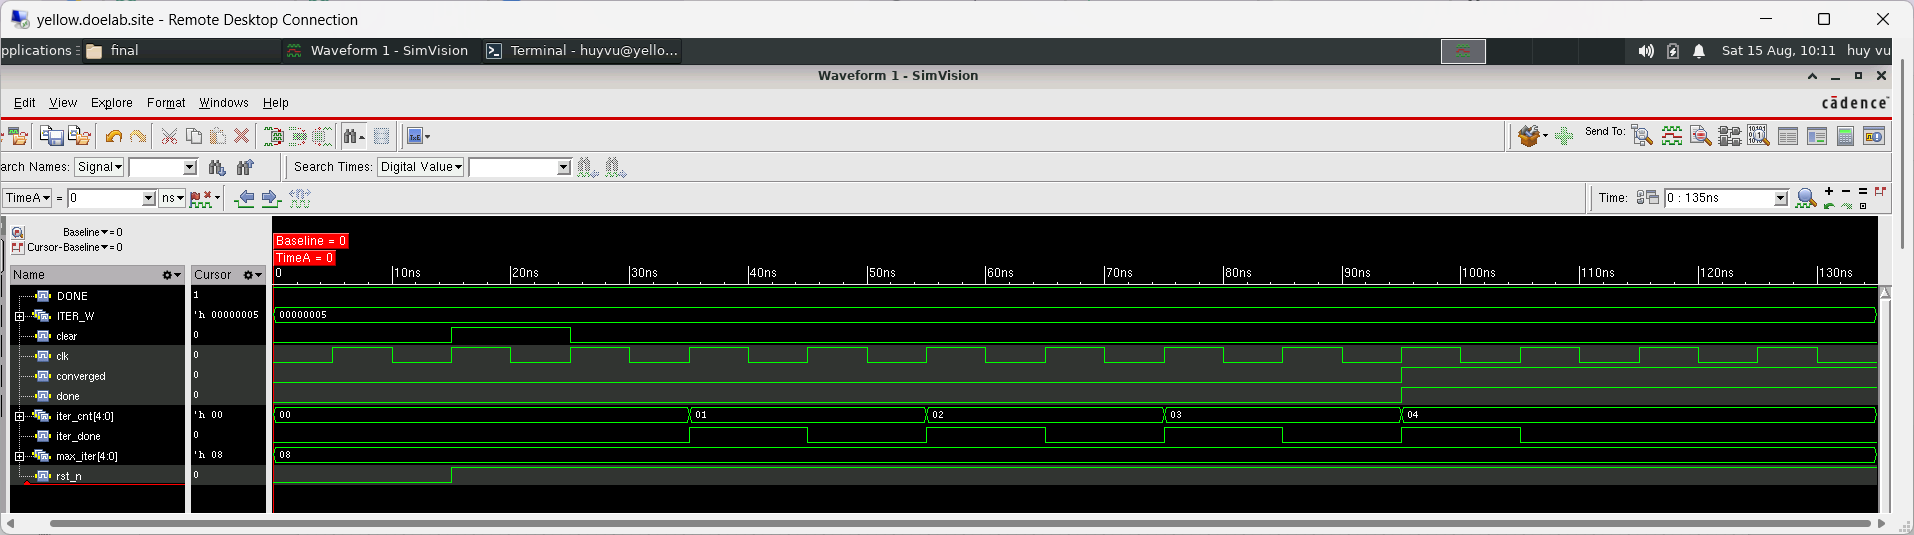
\includegraphics[width=\textwidth]{./images/iter_counter_waveform.png}
    \caption{Dạng sóng của khối Iteration Counter}
\end{figure}
\begin{itemize}
    \item Giai đoạn 1: Khởi động cứng - Từ $0\text{ns}$ đến $\approx 23\text{ns}$. Tín hiệu rst\_n đang ở mức thấp. Hoạt động của mạch: Bất chấp xung nhịp clk dao động, khối điều khiển lập tức ép bộ đếm iter\_cnt về 00 và cờ done về 0 ngay lập tức nhờ cơ chế reset bất đồng bộ (if (!rst\_n)).
    \item Giai đoạn 2: Xóa đồng bộ khung mới - Từ $\approx 35\text{ns}$ đến $\approx 45\text{ns}$rst\_n đã lên mức cao, nhưng tín hiệu clear chuyển lên mức cao trong một vài chu kỳ xung nhịp. Hoạt động của mạch: Mạch thực hiện xóa đồng bộ (else if (clear)), đảm bảo iter\_cnt giữ nguyên ở giá trị 00 và done = 0, sẵn sàng đón nhận khung dữ liệu mã hóa mới mà không cần kích hoạt lại reset toàn cục phần cứng.
    \item Giai đoạn 3: Tiến trình đếm vòng lặp - Sau $\approx 45\text{ns}$ trở đi clear hạ về 0, hệ thống bắt đầu chạy chính thức. max\_iter được thiết lập ở mức 8 (0x08). Hoạt động của mạch: Mỗi khi khối tính toán hoàn thành một vòng lặp, xung iter\_done kích hoạt.iter\_cnt lần lượt tăng giá trị qua từng chu kỳ: từ 00 $\rightarrow$ 01 $\rightarrow$ 02 $\rightarrow$ 03 $\rightarrow$ 04...Kỹ thuật iter\_cnt + 1'b1 trong phần cứng giúp tính trước giá trị vòng lặp kế tiếp để so sánh trực tiếp với max\_iter mà không bị trễ pha clock.
    \item Giai đoạn 4: Hoàn tất và Báo cáo kết quả - Khi iter\_cnt đếm tiệm cận và chạm giới hạn max\_iter (hoặc cờ converged bật lên nếu có tính năng dừng sớm), mạch kích hoạt điều kiện done <= 1'b1. Tín hiệu done chuyển lên mức cao, báo hiệu cho khối lựa chọn chế độ chuyển từ trạng thái Giải mã lặp sang trạng thái Xuất kết quả.
\end{itemize}

Waveform trên minh chứng hoàn toàn chính xác cho thiết kế RTL của khối iteration \_counter: phân tách rành mạch giữa Reset phần cứng (rst\_n) và Xóa khung (clear), đồng thời cơ chế đếm tuần tự phối hợp với thanh ghi max\_iter hoạt động ổn định, đáp ứng đúng chuẩn yêu cầu thời gian của bộ giải mã LDPC.

\begin{table}[H]
\centering
\resizebox{0.8\textwidth}{!}{
\begin{tabular}{|l|c|c|}
\hline
\textbf{Library Name} 
& \textbf{Total Area} 
& \textbf{Total Power} \\
\hline

fast\_vdd1v0\_basicCells\_hvt & 86.184 & 1.74733e-05 \\ \hline
fast\_vdd1v2\_basicCells\_hvt & 86.842 & 2.69313e-05 \\ \hline
slow\_vdd1v0\_basicCells\_hvt & 88.920 & 1.10963e-05 \\ \hline
slow\_vdd1v2\_basicCells\_hvt & 87.552 & 1.75545e-05 \\ \hline
fast\_vdd1v0\_basicCells\_lvt & 85.500 & 2.17925e-05 \\ \hline
fast\_vdd1v2\_basicCells\_lvt & 85.500 & 3.19395e-05 \\ \hline
slow\_vdd1v0\_basicCells\_lvt & 87.552 & 1.35035e-05 \\ \hline
slow\_vdd1v2\_basicCells\_lvt & 85.500 & 1.96727e-05 \\ \hline

\end{tabular}
}
\caption{Tổng hợp thông số Diện tích và Công suất của khối Iteration Counter qua các process corners.}
\end{table}

\textbf{Phân tích Diện tích (Total Area):}
\begin{itemize}
    \item Quy mô siêu nhỏ gọn: Tổng diện tích của khối iteration counter dao động trong khoảng cực kỳ hẹp từ $85.500\,\mu\text{m}^2$ đến $88.920\,\mu\text{m}^2$. Điều này hoàn toàn hợp lý bởi vì đây là một khối điều khiển luồng và đếm vòng lặp, chứa chủ yếu các thanh ghi DFF nhỏ (để lưu iter\_cnt và done), bộ cộng look-ahead đơn giản và các cổng logic tổ hợp so sánh, hoàn toàn không chứa các mảng bộ nhớ lớn hay khối tính toán toán học phức tạp (như VTC hay Min-Sum).
    \item Ảnh hưởng của Thư viện (HVT và LVT): Các góc sử dụng thư viện LVT thường tối ưu hoặc giữ diện tích ở mức tối thiểu ổn định ($85.500\,\mu\text{m}^2$).Các góc sử dụng thư viện HVT có xu hướng nhích nhẹ lên một chút ở một số điều kiện (ví dụ góc slow\_vdd1v0\_basicCells\_hvt đạt đỉnh là $88.920\,\mu\text{m}^2$). Nguyên nhân là do các cell HVT có dòng rò thấp nhưng khả năng chịu tải kém hơn, công cụ tổng hợp buộc phải chèn thêm các cell đệm buffer hoặc chọn các cell có kích thước lớn hơn để đảm bảo thời gian thiết lập tại các góc chậm.
\end{itemize}

\textbf{Phân tích Công suất tiêu thụ (Total Power):}
\begin{itemize}
    \item Mức tiêu thụ công suất của khối nằm trong khoảng từ $1.11 \times 10^{-5}\,\text{W}$ ($11.1\,\mu\text{W}$) đến $3.19 \times 10^{-5}\,\text{W}$ ($31.9\,\mu\text{W}$). Công suất này chịu sự chi phối mạnh mẽ bởi hai yếu tố chính:
    \item Ảnh hưởng của Điện áp cung cấp ($V_{DD}$): Điện áp tăng từ $1.0\text{V}$ lên $1.2\text{V}$ làm công suất tiêu thụ tăng lên đáng kể ở mọi góc thiết kế. Ví dụ: Ở góc fast\_vdd1v0 công suất là $1.75\,\mu\text{W}$, nhưng khi lên góc fast\_vdd1v2, công suất vọt lên $2.69\,\mu\text{W}$ (tăng hơn $50\%$). Điều này tuân theo bản chất vật lý của công suất động ($P_{\text{dynamic}} \propto C \cdot V^2 \cdot f$), trong đó điện áp bình phương đóng vai trò chủ đạo làm tăng mức tiêu thụ năng lượng.
    \item Ảnh hưởng của Loại ngưỡng áp (HVT và LVT): Thư viện LVT luôn tiêu thụ công suất cao hơn so với thư viện HVT tương ứng về mặt điện áp. Ví dụ: Tại góc fast\_vdd1v2, thư viện HVT tiêu thụ $26.9\,\mu\text{W}$, trong khi thư viện LVT đẩy công suất lên tới $31.9\,\mu\text{W}$. Lý do là các transistor LVT có ngưỡng điện áp thấp giúp chuyển mạch nhanh hơn (tối ưu tốc độ) nhưng lại đánh đổi bằng dòng rò lớn hơn và công suất tĩnh/động cao hơn. Ngược lại, HVT là lựa chọn tiết kiệm năng lượng tối ưu cho các thiết kế ưu tiên công suất thấp.
\end{itemize}

\begin{table}[h]
\centering
\resizebox{\textwidth}{!}{%
\begin{tabular}{@{}clp{8.5cm}cc@{}}
\toprule
\textbf{STT} & \textbf{Góc PVT} & \textbf{Đường đi tín hiệu (Critical Path)} & \textbf{Độ trễ (ps)} & \textbf{Thời gian dư (ps)} \\ \midrule
1 & fast\_1v0\_hvt & max\_iter[1] $\rightarrow$ OAI211X1HVT $\rightarrow$ OAI221X1HVT $\rightarrow$ OAI221X1HVT $\rightarrow$ OAI221X1HVT $\rightarrow$ OAI221X1HVT $\rightarrow$ OA21X1HVT $\rightarrow$ AOI2BB1XLHVT $\rightarrow$ done\_reg/D & 240 & 1226 \\
2 & fast\_1v2\_hvt & max\_iter[1] $\rightarrow$ OAI211X1HVT $\rightarrow$ OAI221X1HVT $\rightarrow$ OAI221X1HVT $\rightarrow$ OAI221X1HVT $\rightarrow$ OAI221XLHVT $\rightarrow$ OA21X1HVT $\rightarrow$ AOI221X1HVT $\rightarrow$ done\_reg/D & 163 & 1316 \\
3 & slow\_1v0\_hvt & iter\_cnt\_reg[0]/CK $\rightarrow$ DFFRX1HVT $\rightarrow$ NAND2X1HVT $\rightarrow$ NOR2BX1HVT $\rightarrow$ AND2XLHVT $\rightarrow$ AOI2BB1X1HVT $\rightarrow$ NOR2X1HVT $\rightarrow$ OAI221X1HVT $\rightarrow$ OAI221X1HVT $\rightarrow$ OAI221X1HVT $\rightarrow$ OAI21XLHVT $\rightarrow$ OA21X1HVT $\rightarrow$ done\_reg/D & 1772 & 4 \\
4 & slow\_1v2\_hvt & max\_iter[0] $\rightarrow$ NAND2BXLHVT $\rightarrow$ AOI2BB1XLHVT $\rightarrow$ AOI21XLHVT $\rightarrow$ OAI22X1HVT $\rightarrow$ OAI221X1HVT $\rightarrow$ OAI221X1HVT $\rightarrow$ OA21X1HVT $\rightarrow$ AOI2BB1XLHVT $\rightarrow$ done\_reg/D & 556 & 909 \\
5 & fast\_1v0\_lvt & max\_iter[1] $\rightarrow$ OAI211X1LVT $\rightarrow$ OAI221X1LVT $\rightarrow$ OAI221X1LVT $\rightarrow$ OAI221X1LVT $\rightarrow$ OAI221X1LVT $\rightarrow$ AOI2BB1X1LVT $\rightarrow$ OA21X1LVT $\rightarrow$ AOI2BB1X1LVT $\rightarrow$ done\_reg/D & 129 & 1356 \\
6 & fast\_1v2\_lvt & max\_iter[1] $\rightarrow$ OAI211X1LVT $\rightarrow$ OAI221X1LVT $\rightarrow$ OAI221X1LVT $\rightarrow$ OAI221X1LVT $\rightarrow$ OAI221X1LVT $\rightarrow$ AOI2BB1X1LVT $\rightarrow$ OA21X1LVT $\rightarrow$ AOI2BB1X1LVT $\rightarrow$ done\_reg/D & 102 & 1387 \\
7 & slow\_1v0\_lvt & max\_iter[0] $\rightarrow$ NAND2BXLVT $\rightarrow$ OAI221X1LVT $\rightarrow$ AOI21X1LVT $\rightarrow$ OAI22X1LVT $\rightarrow$ OAI221X1LVT $\rightarrow$ OAI221X1LVT $\rightarrow$ OA21X1LVT $\rightarrow$ AOI2BB1X1LVT $\rightarrow$ done\_reg/D & 509 & 959 \\
8 & slow\_1v2\_lvt & max\_iter[1] $\rightarrow$ OAI211X1LVT $\rightarrow$ OAI221X1LVT $\rightarrow$ OAI221X1LVT $\rightarrow$ OAI221X1LVT $\rightarrow$ OAI221X1LVT $\rightarrow$ AOI2BB1X1LVT $\rightarrow$ OA21X1LVT $\rightarrow$ AOI2BB1X1LVT $\rightarrow$ done\_reg/D & 313 & 1146 \\ \bottomrule
\end{tabular}%
}
\caption{Thống kê độ trễ các góc phân tích (PVT corners) cho khối iteration\_counter.}
\end{table}

\begin{itemize}
    \item Đặc điểm kiến trúc và Đường đi tới hạn: Khối iteration\_counter thực hiện việc đếm số vòng lặp giải mã (iter\_cnt), kết hợp kỹ thuật tính toán iter\_cnt + 1'b1 để so sánh trực tiếp với max\_iter nhằm cập nhật cờ done ngay trong chu kỳ mà vòng lặp kết thúc mà không bị trễ chu kỳ. Quá trình phân tích chỉ ra hai dạng đường đi tới hạn chính: 
    \begin{itemize}
        \item Dạng đường đi từ ngõ vào cấu hình (max\_iter): Đa số các góc phân tích có đường đi bắt đầu từ các bít ngõ vào max\_iter[0] hoặc max\_iter[1], đi qua các tầng logic tổ hợp so sánh kích thước (chuỗi cổng OAI, AOI, NAND) để đến chân D của thanh ghi done\_reg. Do có input\_delay = 400\,\text{ps}, độ trễ dữ liệu (Data Path) dao động từ $102\,\text{ps}$ đến $556\,\text{ps}$, giúp các góc này đạt thời gian dư (Slack) rất lớn (từ $909\,\text{ps}$ đến $1387\,\text{ps}$).
        \item Dạng đường đi từ thanh ghi nội bộ (slow\_1v0\_hvt): Tại góc khắc nghiệt nhất slow\_1v0\_hvt ($0.9\text{V}$, $125^\circ\text{C}$ với thư viện HVT), đường đi tới hạn chuyển dịch xuất phát từ chân clock của thanh ghi nội bộ iter\_cnt\_reg[0]/CK, đi qua toàn bộ khối cộng/incrementer và chuỗi logic so sánh phức tạp (NAND, NOR, AND, OAI, AOI) tới done\_reg/D. Độ trễ dữ liệu vọt lên mức $1772\,\text{ps}$, khiến thời gian dư thu hẹp nghiêm trọng chỉ còn $4\,\text{ps}$. Điều này cho thấy mạch hoạt động sát nút giới hạn setup time tại điều kiện nhiệt độ cao và điện áp thấp.
    \end{itemize}
    \item Các góc sử dụng thư viện LVT cải thiện đáng kể tốc độ chuyển mạch, giữ cho Data Path ở mức thấp và Slack rất an toàn. Ngược lại, thư viện HVT chịu sự suy giảm hiệu năng mạnh ở điều kiện áp thấp/nhiệt độ cao, đòi hỏi phải kiểm tra cẩn thận nếu hệ thống vận hành ở môi trường khắc nghiệt.
\end{itemize}

\section{Khối Mode Select}
Bước đầu ta sẽ khảo sát dạng sóng waveform của thiết kế khối này.
\begin{figure}[h!]
    \centering
    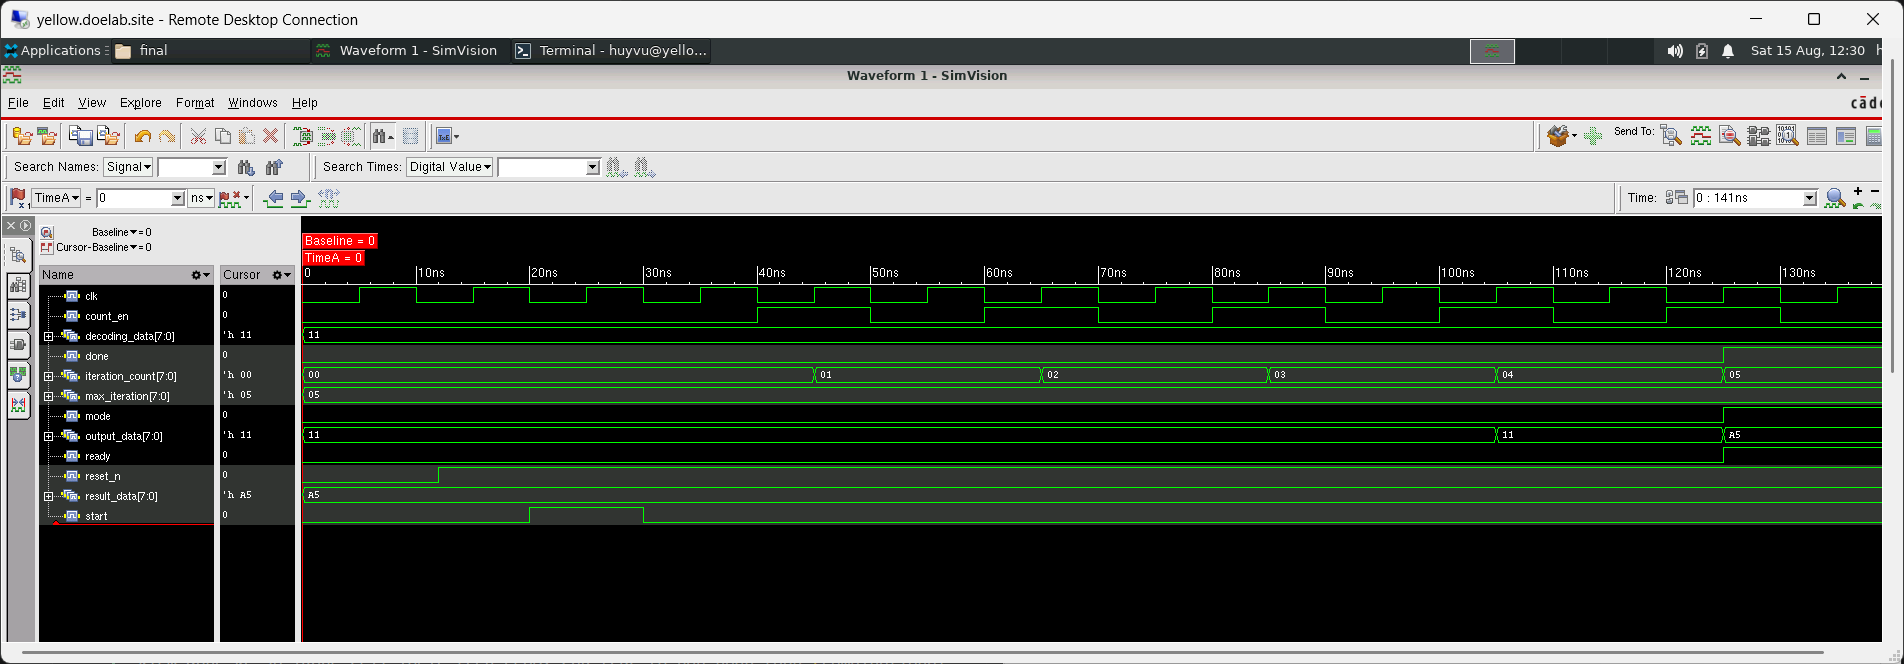
\includegraphics[width=\textwidth]{./images/mode_select_waveform.png}
    \caption{Dạng sóng của khối Mode Select}
\end{figure}
\begin{itemize}
    \item Giai đoạn 1: Khởi động cứng — Từ $0\text{ns}$ đến $\approx 12\text{ns}$. Tín hiệu reset\_n đang ở mức thấp. Hoạt động của mạch: Dù xung nhịp clk dao động, tín hiệu reset bất đồng bộ ép iteration\_count về 'h 00. Cờ done, mode và ready đều giữ mức 0. Ngõ ra output\_data đang chọn kênh decoding\_data với giá trị 'h 11.
    \item Giai đoạn 2: Xung kích hoạt khởi động (start) — Từ $\approx 22\text{ns}$ đến $\approx 35\text{ns}$, reset\_n đã lên mức cao, và một xung mức cao xuất hiện trên tín hiệu start. Hoạt động của mạch: Theo thiết kế của iteration\_counter, khi tín hiệu start được kích hoạt, bộ đếm được đồng bộ hóa và giữ hoặc đưa về giá trị 'h00, chuẩn bị sẵn sàng cho quá trình đếm vòng lặp giải mã.
    \item Giai đoạn 3: Tiến trình đếm vòng lặp — Từ $\approx 43\text{ns}$ đến $\approx 125\text{ns}$, start hạ về 0, hệ thống tiến hành đếm qua từng chu kỳ xung nhịp clk: Tại $\approx 43\text{ns}$: iteration\_count tăng lên 'h 01.Tiếp tục tăng đều qua các mốc thời gian tiếp theo: 'h 02, 'h 03, 'h 04.Hoạt động so sánh: Bộ so sánh iter\_compare sử dụng khối fa\_calc (với Sel = 1'b1) để liên tục tính toán độ lệch giữa iteration\_count và max\_iteration ('h 05). Trong suốt giai đoạn này, iteration\_count vẫn nhỏ hơn max\_iteration, do đó cờ done giữ nguyên mức 0. 
    \item Giai đoạn 4: Hoàn tất quá trình và Chuyển chế độ (Done \& Result Output) — Từ $\approx 125\text{ns}$ trở đi khi iteration\_count đếm đến giá trị 'h 05, chạm ngưỡng max\_iteration:Cờ done chuyển từ mức thấp  lên mức cao.  Do assign mode = done và assign ready = done, các tín hiệu mode và ready đồng thời chuyển lên mức cao.  Chuyển kênh dữ liệu ngõ ra:Khi mode = 1, bộ ghép kênh (MUX) tự động chuyển đổi ngõ ra output\_data từ decoding\_data ('h 11) sang result\_data ('h A5).  Tín hiệu ready = 1 phát đi thông báo rằng quá trình giải mã đã hoàn tất và kết quả đã sẵn sàng xuất ra hệ thống phía sau.  
\end{itemize}

Waveform mô phỏng hoàn toàn trùng khớp với logic thiết kế của file mode\_select\_top.sv: mạch hoạt động tuần tự, đếm chính xác số vòng lặp từ 00 đến 05, và tự động chuyển đổi trạng thái (done, mode, ready) cũng như chuyển mạch dữ liệu ngõ ra (output\_data) ngay khi chạm mốc giới hạn cấu hình max\_iteration.

\begin{table}[H]
\centering
\resizebox{0.8\textwidth}{!}{
\begin{tabular}{|l|c|c|}
\hline
\textbf{Library Name} 
& \textbf{Total Area} 
& \textbf{Total Power} \\
\hline

fast\_vdd1v0\_basicCells\_hvt & 86.184 & 1.74733e-05 \\ \hline
fast\_vdd1v2\_basicCells\_hvt & 86.842 & 2.69313e-05 \\ \hline
slow\_vdd1v0\_basicCells\_hvt & 88.920 & 1.10963e-05 \\ \hline
slow\_vdd1v2\_basicCells\_hvt & 87.552 & 1.75545e-05 \\ \hline
fast\_vdd1v0\_basicCells\_lvt & 85.500 & 2.17925e-05 \\ \hline
fast\_vdd1v2\_basicCells\_lvt & 85.500 & 3.19395e-05 \\ \hline
slow\_vdd1v0\_basicCells\_lvt & 87.552 & 1.35035e-05 \\ \hline
slow\_vdd1v2\_basicCells\_lvt & 85.500 & 1.96727e-05 \\ \hline

\end{tabular}
}
\caption{Tổng hợp thông số Diện tích và Công suất của khối Mode Select qua các process corners.}
\end{table}

\textbf{Phân tích Diện tích (Total Area):}
\begin{itemize}
    \item Quy mô tối ưu và nhỏ gọn: Tổng diện tích của khối Mode Select dao động trong một khoảng rất hẹp, từ $85.500\,\mu\text{m}^2$ đến $88.920\,\mu\text{m}^2$. Đây là mức diện tích hoàn toàn phù hợp đối với một khối điều khiển logic thuần túy, chủ yếu bao gồm các thanh ghi DFF (lưu trữ giá trị biến đếm iter\_cnt và cờ done), cùng một bộ cộng/so sánh look-ahead nhỏ gọn. Khối này không chứa các mảng bộ nhớ lớn hay các khối toán học phức tạp, do đó chiếm diện tích không đáng kể so với toàn bộ kiến trúc bộ giải mã LDPC.
    \item Ảnh hưởng của HVT và LVT: Các góc sử dụng thư viện LVT duy trì diện tích ở mức tối thiểu ổn định là $85.500\,\mu\text{m}^2$ ở hầu hết các điều kiện.Các góc sử dụng thư viện HVT có xu hướng nhích nhẹ lên một chút (đạt đỉnh ở góc slow\_vdd1v0\_basicCells\_ hvt với $88.920\,\mu\text{m}^2$). Nguyên nhân là do các cell HVT có dòng điện truyền qua nhỏ hơn (tốc độ chậm hơn), buộc công cụ tổng hợp như Genus phải tự động điều chỉnh tăng kích thước cell hoặc chèn thêm các cell đệm nhằm đảm bảo các ràng buộc về thời gian thiết lập tại các góc vận hành chậm.
\end{itemize}

\textbf{Phân tích Công suất tiêu thụ (Total Power):}
\begin{itemize}
    \item Ảnh hưởng trực tiếp của Điện áp cung cấp ($V_{DD}$):Khi điện áp tăng từ $1.0\text{V}$ lên $1.2\text{V}$, công suất tiêu thụ của mạch tăng lên đáng kể ở tất cả các nhóm thư viện.Ví dụ cụ thể (với nhóm HVT): Ở góc điện áp thấp fast\_vdd1v0\_basicCells\_hvt, công suất tiêu thụ là $17.47\,\mu\text{W}$, nhưng khi nâng điện áp lên $1.2\text{V}$ (fast\_vdd1v2\_basicCells\_hvt), công suất vọt lên mức $26.93\,\mu\text{W}$ (tăng hơn $54\%$).
    \item Ảnh hưởng của loại ngưỡng điện áp transistor (HVT và LVT): Các góc sử dụng thư viện LVT luôn tiêu tốn nhiều năng lượng hơn so với các góc dùng thư viện HVT tương ứng về mặt điện áp. Ví dụ: Ở điều kiện fast\_vdd1v2, thư viện HVT tiêu thụ $26.93\,\mu\text{W}$, trong khi thư viện LVT đẩy mức công suất lên tới $31.94\,\mu\text{W}$. Transistor LVT có dòng rò lớn hơn và cấu trúc chuyển mạch nhanh hơn, đánh đổi bằng việc tiêu thụ năng lượng cao hơn. Ngược lại, thư viện HVT thể hiện ưu thế tiết kiệm điện năng rõ rệt, phù hợp cho các thiết kế ưu tiên tiêu thụ công suất thấp.
\end{itemize}

\begin{table}[h]
\centering
\resizebox{0.9\textwidth}{!}{%
\begin{tabular}{@{}clp{8.5cm}cc@{}}
\toprule
\textbf{STT} & \textbf{Góc PVT} & \textbf{Đường đi tín hiệu (Critical Path)} & \textbf{Độ trễ (ps)} & \textbf{Thời gian dư (ps)} \\ \midrule
1 & fast\_1v0\_hvt & max\_iteration[0] $\rightarrow$ INVX1HVT $\rightarrow$ OR2XLHVT $\rightarrow$ OAI21X1HVT $\rightarrow$ OAI2BB1X1HVT $\rightarrow$ OAI21X1HVT $\rightarrow$ OAI2BB1X1HVT $\rightarrow$ OAI21X1HVT $\rightarrow$ OAI2BB1X1HVT $\rightarrow$ BUFX2HVT $\rightarrow$ ready & 877 & 223 \\
2 & fast\_1v2\_hvt & max\_iteration[0] $\rightarrow$ INVX1HVT $\rightarrow$ OR2XLHVT $\rightarrow$ OAI21X1HVT $\rightarrow$ OAI2BB1X1HVT $\rightarrow$ OAI21X1HVT $\rightarrow$ OAI2BB1X1HVT $\rightarrow$ OAI21X1HVT $\rightarrow$ OAI2BB1X1HVT $\rightarrow$ CLKMX2HVT $\rightarrow$ output\_data[0] & 594 & 506 \\
3 & slow\_1v0\_hvt & max\_iteration[0] $\rightarrow$ CLKINVX12HVT $\rightarrow$ NOR2X8HVT $\rightarrow$ CLKINVX6HVT $\rightarrow$ NAND2X4HVT $\rightarrow$ NAND2X4HVT $\rightarrow$ NAND2X4HVT $\rightarrow$ NAND2X4HVT $\rightarrow$ NAND2X2HVT $\rightarrow$ NAND2X1HVT $\rightarrow$ OAI2BB1X1HVT $\rightarrow$ NAND2X8HVT $\rightarrow$ AND2X1HVT $\rightarrow$ OR2X8HVT $\rightarrow$ output\_data[0] & 1871 & -771 \\
4 & slow\_1v2\_hvt & max\_iteration[0] $\rightarrow$ INVX1HVT $\rightarrow$ OR2XLHVT $\rightarrow$ AO22XLHVT $\rightarrow$ OAI21X1HVT $\rightarrow$ OAI2BB1X1HVT $\rightarrow$ OAI21X1HVT $\rightarrow$ OAI2BB1X1HVT $\rightarrow$ OAI21X1HVT $\rightarrow$ OAI2BB1X1HVT $\rightarrow$ CLKMX2HVT $\rightarrow$ output\_data[0] & 1096 & 4 \\
5 & fast\_1v0\_lvt & max\_iteration[0] $\rightarrow$ INVXLVT $\rightarrow$ OR2XLVT $\rightarrow$ OAI21X1LVT $\rightarrow$ OAI2BB1X1LVT $\rightarrow$ OAI21X1LVT $\rightarrow$ OAI2BB1X1LVT $\rightarrow$ OAI21X1LVT $\rightarrow$ OAI2BB1X1LVT $\rightarrow$ CLKMX2LVT $\rightarrow$ output\_data[0] & 480 & 620 \\
6 & fast\_1v2\_lvt & max\_iteration[0] $\rightarrow$ INVXLVT $\rightarrow$ OR2XLVT $\rightarrow$ OAI21X1LVT $\rightarrow$ OAI2BB1X1LVT $\rightarrow$ OAI21X1LVT $\rightarrow$ OAI2BB1X1LVT $\rightarrow$ OAI21X1LVT $\rightarrow$ OAI2BB1X1LVT $\rightarrow$ CLKMX2LVT $\rightarrow$ output\_data[0] & 479 & 621 \\
7 & slow\_1v0\_lvt & max\_iteration[0] $\rightarrow$ INVXLVT $\rightarrow$ OR2XLVT $\rightarrow$ OAI21X1LVT $\rightarrow$ OAI2BB1X1LVT $\rightarrow$ OAI21X1LVT $\rightarrow$ OAI2BB1X1LVT $\rightarrow$ OAI21X1LVT $\rightarrow$ OAI2BB1X1LVT $\rightarrow$ CLKMX2LVT $\rightarrow$ output\_data[0] & 1056 & 44 \\
8 & slow\_1v2\_lvt & max\_iteration[0] $\rightarrow$ INVXLVT $\rightarrow$ OR2XLVT $\rightarrow$ OAI21X1LVT $\rightarrow$ OAI2BB1X1LVT $\rightarrow$ OAI21X1LVT $\rightarrow$ OAI2BB1X1LVT $\rightarrow$ OAI21X1LVT $\rightarrow$ OAI2BB1X1LVT $\rightarrow$ ready & 717 & 383 \\ \bottomrule
\end{tabular}%
}
\caption{Thống kê độ trễ các góc phân tích (PVT corners) cho khối mode\_select.}
\end{table}

\begin{itemize}
    \item Tất cả các đường đi tới hạn (critical paths) đều bắt đầu từ thanh ghi hoặc cổng đầu vào max\_iteration[0] và đi tới các tín hiệu ngõ ra như ready hoặc output\_data[0].
    \item Góc Fast (FF): Cả 4 góc fast (fast\_1v0\_hvt, fast\_1v2\_hvt, fast\_1v0\_lvt, fast\_1v2 \_lvt) đều đạt timing rất tốt, với thời gian dư (slack) dương lớn (từ 223 ps đến 621 ps), trong đó các cell LVT cho tốc độ phản hồi nhanh hơn đáng kể so với HVT.
    \item Góc Slow (SS): Góc ảnh hướng nhất slow\_1v0\_hvt (điện áp thấp 1.0V và cell HVT) gặp hiện tượng vi phạm timing nghiêm trọng với độ trễ đường dữ liệu lên tới 1871 ps và âm slack -771 ps (VIOLATED). Tuy nhiên, khi tăng điện áp lên 1.2V (slow\_1v2\_hvt) hoặc chuyển sang công nghệ LVT (slow\_1v0\_lvt, slow\_1v2\_lvt), mạch đã vượt qua giới hạn timing thành công (MET) với các khoảng slack dương (4 ps, 44 ps, 383 ps).
\end{itemize}

\section{Khối VTC Calculation}
Bước đầu ta sẽ khảo sát dạng sóng waveform của thiết kế khối này.
\begin{figure}[h!]
    \centering
    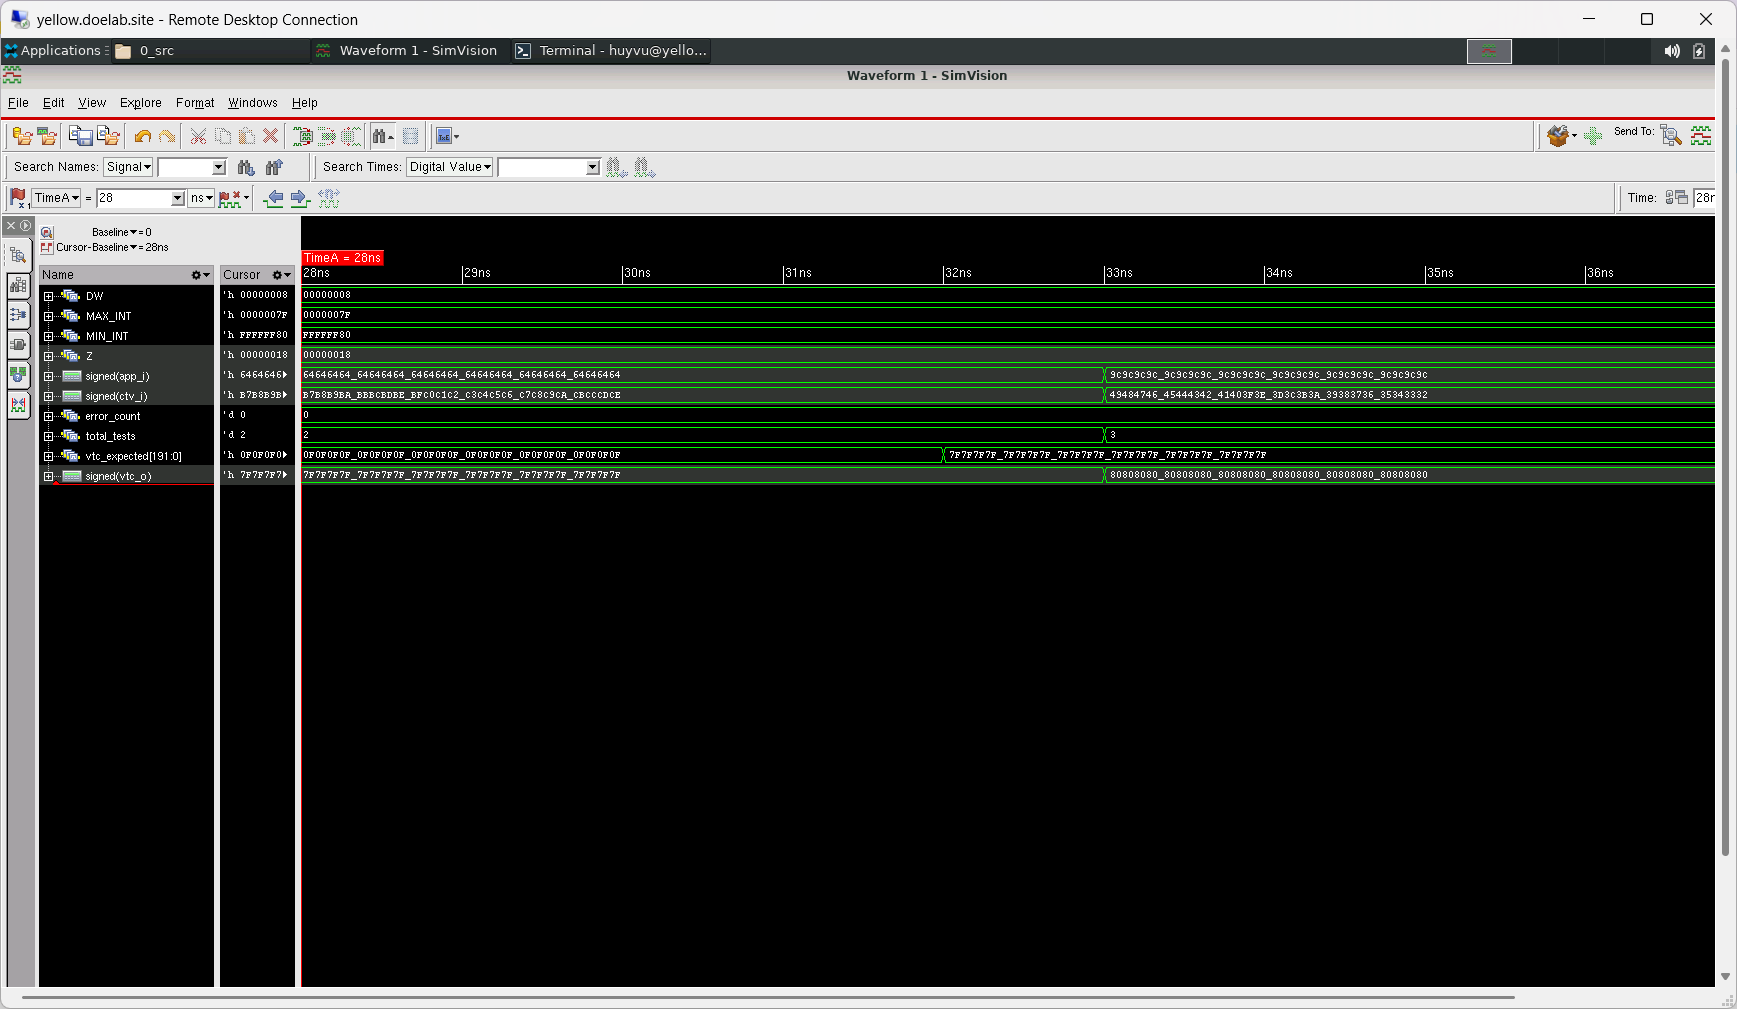
\includegraphics[width=\textwidth]{./images/vtc_calc_waveform.png}
    \caption{Dạng sóng của khối VTC Calculation}
\end{figure}
\begin{itemize}
    \item Dữ liệu đầu vào (app\_i \& ctv\_i): app\_i: Giá trị 24 byte song song xếp từ 0x14 (20) ở kênh 0 đến 0x2B (43) ở kênh 23. ctv\_i: Giá trị 24 byte tương ứng từ 0x05 (5) ở kênh 0 đến 0x1C (28) ở kênh 23.
    \item Kết quả tính toán RTL (vtc\_o): Phép trừ $app\_i[i] - ctv\_i[i]$ cho hiệu số trên mọi kênh song song luôn bằng $20 - 5 = 15$ (0x0F). Mạch tổ hợp (always\_comb) cập nhật đầu ra ngay lập tức thành chuỗi 0F0F0F0F...0F0F0F0F tại 10 ns.
    \item Lý do lệch pha thời gian của vtc\_expected: Trong khoảng 10 ns - 20 ns, vtc\_expected giữ giá trị 0000...00 do task check\_outputs chỉ được gọi để tính toán mô hình tham chiếu tại thời điểm kết thúc chu kỳ (20 ns). Đến mốc 20 ns, vtc\_expected cập nhật sang 0F0F...0F trùng khớp 100\% với vtc\_o.
\end{itemize}

\begin{table}[H]
\centering
\resizebox{0.8\textwidth}{!}{
\begin{tabular}{|l|c|c|}
\hline
\textbf{Library Name} 
& \textbf{Total Area} 
& \textbf{Total Power} \\
\hline

fast\_vdd1v0\_basicCells\_hvt & 1690.848 & 1.89295e-03 \\ \hline
fast\_vdd1v2\_basicCells\_hvt & 1690.848 & 2.75025e-03 \\ \hline
slow\_vdd1v0\_basicCells\_hvt & 5283.174 & 1.56203e-03 \\ \hline
slow\_vdd1v2\_basicCells\_hvt & 2708.640 & 2.29457e-03 \\ \hline
fast\_vdd1v0\_basicCells\_lvt & 1690.848 & 1.96594e-03 \\ \hline
fast\_vdd1v2\_basicCells\_lvt & 1567.728 & 2.71340e-03 \\ \hline
slow\_vdd1v0\_basicCells\_lvt & 2093.040 & 1.37146e-03 \\ \hline
slow\_vdd1v2\_basicCells\_lvt & 1822.176 & 1.96337e-03 \\ \hline

\end{tabular}
}
\caption{Tổng hợp thông số Diện tích và Công suất của khối VTC Calculation qua các process corners.}
\end{table}

\textbf{Phân tích Diện tích (Total Area):}
\begin{itemize}
    \item Diện tích lớn nhất ($5283.174\,\mu\text{m}^2$): Xuất hiện tại góc kém nhất slow\_vdd1v0\_basicCells\_hvt. Ở điều kiện quy trình chậm (slow process), điện áp thấp ($V_{DD} = 1.0\,\text{V}$) và điện áp ngưỡng cao (HVT), dòng dẫn của transistor suy giảm mạnh. Công cụ tổng hợp buộc phải tăng kích thước cell (gate upsizing) hoặc thêm các buffer/logic song song để thỏa mãn ràng buộc thời gian (timing constraint), làm diện tích tăng lên gấp khoảng $3.1\times$ so với corner tối ưu.
    \item Diện tích nhỏ nhất ($1567.728\,\mu\text{m}^2$): Đạt được tại corner fast\_vdd1v2\_basicCells\_lvt. Quy trình sản xuất nhanh, điện áp cao ($V_{DD} = 1.2\,\text{V}$) cùng điện áp ngưỡng thấp (LVT) giúp dòng drive của các cell đạt mức tối đa, cho phép công cụ tổng hợp dùng hầu hết các cell kích thước tối thiểu (minimum sizing) mà vẫn đáp ứng timing.
    \item Ảnh hưởng của điện áp ($V_{DD}$): Tăng $V_{DD}$ từ $1.0\,\text{V}$ lên $1.2\,\text{V}$ ở góc slow giúp giảm mạnh diện tích (đối với HVT giảm từ $5283.174$ xuống $2708.640\,\mu\text{m}^2$) do dòng dẫn cải thiện đáng kể.
\end{itemize}

\textbf{Phân tích Công suất tiêu thụ (Total Power):}
\begin{itemize}
    \item Công suất cao nhất ($2.75025 \times 10^{-3}\,\text{W} \approx 2.75\,\text{mW}$): Xuất hiện tại fast\_vdd1v2 \_basicCells\_hvt (và $2.713\,\text{mW}$ ở LVT). Công suất thấp nhất ($1.37146 \times 10^{-3}\,\text{W} \approx 1.37\,\text{mW}$): Đạt được ở corner slow\_vdd1v0\_basicCells\_lvt. Việc hạ điện áp nguồn xuống $V_{DD} = 1.0\,\text{V}$ giúp giảm trực tiếp cả công suất động $P_{dyn}$ và công suất rò tĩnh $P_{leak}$.
    \item Tại Fast Corner: Thư viện LVT tiêu thụ công suất cao hơn HVT (ở $1.0\,\text{V}$ là $1.966\,\text{mW}$ so với $1.893\,\text{mW}$) do dòng rò tĩnh ($I_{leakage}$) của transistor LVT ở điều kiện fast tăng vọt.
    \item Tại Slow Corner: Thư viện HVT lại tiêu thụ tổng công suất lớn hơn LVT (ở $1.0\,\text{V}$ là $1.562\,\text{mW}$ so với $1.371\,\text{mW}$). Nguyên nhân do ở góc slow, mạch dùng HVT bị tăng kích thước cell quá lớn (diện tích gấp 2.5 lần), kéo theo điện dung ký sinh ($C_{load}$) tăng mạnh và làm công suất động áp đảo hoàn toàn công suất rò.
\end{itemize}
\newpage
\begin{table}[h]
\centering
\resizebox{\textwidth}{!}{%
\begin{tabular}{@{}clp{8.5cm}cc@{}}
\toprule
\textbf{STT} & \textbf{Góc PVT} & \textbf{Đường đi tín hiệu (Critical Path)} & \textbf{Độ trễ (ps)} & \textbf{Thời gian dư (ps)} \\ \midrule
1 & fast\_1v0\_hvt & ctv\_i[23][0] $\rightarrow$ NAND2BX1HVT $\rightarrow$ ADDFX1HVT ($\times 6$) $\rightarrow$ INVX1HVT $\rightarrow$ AO21X2HVT $\rightarrow$ NAND2BX1HVT $\rightarrow$ AO21X2HVT $\rightarrow$ vtc\_o[23][0] & 987 & 213 \\
2 & fast\_1v2\_hvt & ctv\_i[23][0] $\rightarrow$ NAND2BX1HVT $\rightarrow$ ADDFX1HVT ($\times 6$) $\rightarrow$ INVX1HVT $\rightarrow$ AO21X2HVT $\rightarrow$ NAND2BX1HVT $\rightarrow$ AO21X2HVT $\rightarrow$ vtc\_o[23][0] & 691 & 509 \\
3 & slow\_1v0\_hvt & app\_i[20][0] $\rightarrow$ CLKINVX12HVT $\rightarrow$ NAND2X8HVT $\rightarrow$ NOR2X4HVT ($\times 2$) $\rightarrow$ NOR2X2HVT $\rightarrow$ NOR2X4HVT $\rightarrow$ NOR2X2HVT $\rightarrow$ NOR3BX1HVT $\rightarrow$ AOI2BB1X4HVT $\rightarrow$ NOR2X1HVT $\rightarrow$ OR2X8HVT $\rightarrow$ vtc\_o[20][0] & 1220 & -20 \\
4 & slow\_1v2\_hvt & app\_i[23][0] $\rightarrow$ NAND2BX1HVT $\rightarrow$ ADDFX1HVT $\rightarrow$ NAND3X1HVT $\rightarrow$ NAND2X1HVT $\rightarrow$ NAND3X1HVT $\rightarrow$ AND2X6HVT $\rightarrow$ NAND2BX1HVT $\rightarrow$ OR2X6HVT $\rightarrow$ vtc\_o[23][0] & 1054 & 146 \\
5 & fast\_1v0\_lvt & ctv\_i[23][0] $\rightarrow$ NAND2BX1LVT $\rightarrow$ ADDFX1LVT ($\times 6$) $\rightarrow$ INVXLLVT $\rightarrow$ AO21X2LVT $\rightarrow$ NAND2BX1LVT $\rightarrow$ AO21X2LVT $\rightarrow$ vtc\_o[23][0] & 523 & 677 \\
6 & fast\_1v2\_lvt & ctv\_i[23][0] $\rightarrow$ NAND2BX1LVT $\rightarrow$ ADDFX1LVT ($\times 6$) $\rightarrow$ INVXLLVT $\rightarrow$ AO21X2LVT $\rightarrow$ NAND2BX1LVT $\rightarrow$ AO21X2LVT $\rightarrow$ vtc\_o[23][0] & 554 & 646 \\
7 & slow\_1v0\_lvt & ctv\_i[23][1] $\rightarrow$ INVX2LVT $\rightarrow$ NOR2X1LVT $\rightarrow$ OAI21X1LVT $\rightarrow$ OAI2BB1X1LVT $\rightarrow$ ADDFX1LVT ($\times 4$) $\rightarrow$ NOR2X1LVT $\rightarrow$ OR2X6LVT $\rightarrow$ NOR2BX1LVT $\rightarrow$ vtc\_o[23][0] & 1198 & 2 \\
8 & slow\_1v2\_lvt & app\_i[23][0] $\rightarrow$ NAND2BX1LVT $\rightarrow$ ADDFX1LVT ($\times 6$) $\rightarrow$ INVX1LVT $\rightarrow$ AO21X2LVT $\rightarrow$ NAND2BX1LVT $\rightarrow$ AO21X2LVT $\rightarrow$ vtc\_o[23][0] & 887 & 313 \\ \bottomrule
\end{tabular}%
}
\caption{Thống kê độ trễ các góc phân tích (PVT corners) cho khối vtc\_calc.}
\end{table}

\begin{itemize}
    \item Điểm bắt đầu (Startpoint) và Kết thúc (Endpoint): Các đường dẫn tới hạn (critical paths) trong khối vtc\_calc chủ yếu xuất phát từ các cổng dữ liệu ngõ vào như ctv\_i hoặc app\_i và kết thúc tại ngõ ra vtc\_o.
    \item Góc Fast (FF): Cả 4 góc fast (fast\_1v0\_hvt, fast\_1v2\_hvt, fast\_1v0\_lvt, fast\_1v2\_lvt) đều đạt kết quả rất tốt (MET) với thời gian dư (slack) dương lớn (từ 213 ps đến 677 ps). Các cell công nghệ LVT tiếp tục thể hiện tốc độ phản hồi nhanh hơn đáng kể so với HVT.
    \item Góc Slow (SS): Góc ảnh hưởng nhất slow\_1v0\_hvt (điện áp thấp 0.9V, nhiệt độ cao 125°C, cell HVT) gặp hiện tượng vi phạm timing nhẹ với độ trễ đường dữ liệu là 1220 ps và âm slack -20 ps (VIOLATED). Tuy nhiên, khi nâng điện áp lên 1.08V (slow\_1v2\_hvt) hoặc chuyển đổi sang cấu trúc cell LVT (slow\_1v0\_lvt, slow\_1v2\_lvt), toàn bộ các góc slow còn lại đều vượt qua giới hạn timing thành công (MET) với các khoảng slack dương tương ứng (2 ps, 146 ps, và 313 ps).
\end{itemize}
\newpage
\section{Khối Min/Submin Calculation}
Bước đầu ta sẽ khảo sát dạng sóng waveform của thiết kế khối này.
\begin{figure}[h!]
    \centering
    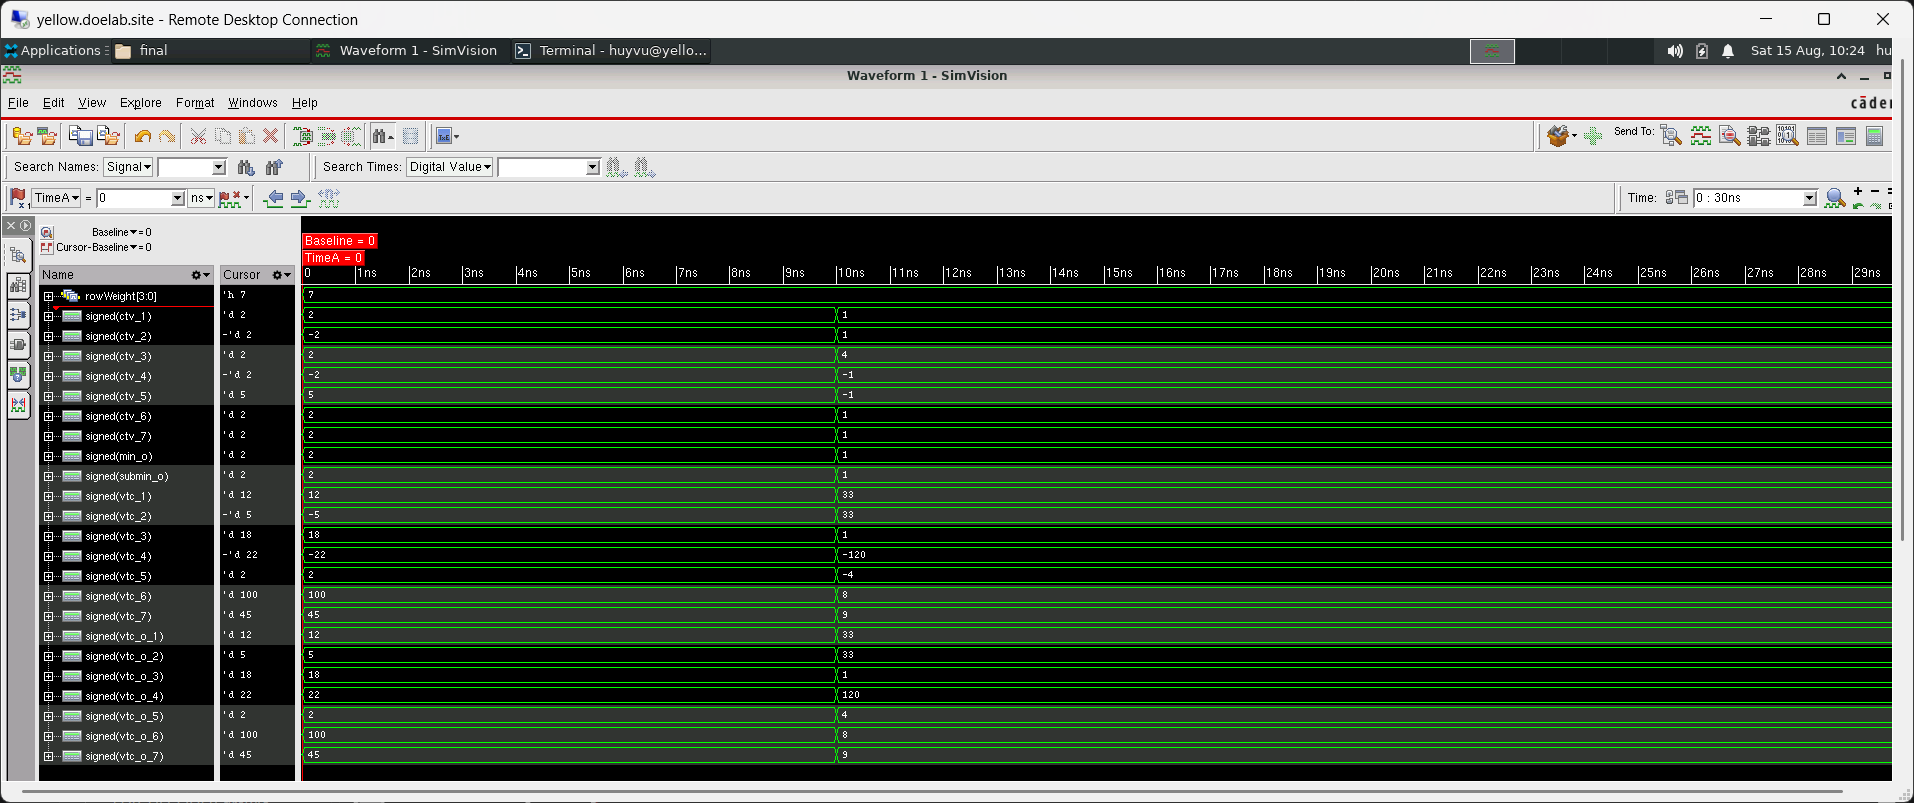
\includegraphics[width=\textwidth]{./images/min_submin_waveform.png}
    \caption{Dạng sóng của khối Min Submin Calculation}
\end{figure}
\begin{itemize}
    \item \textit{Giai đoạn 1: Phân tách hai giá trị nhỏ nhất biệt lập (Mốc 10 ns)}. Tín hiệu ngõ vào: Tập dữ liệu mang giá trị nhỏ nhất $X_3 = 1$ và nhỏ nhì $X_5 = 4$. Diễn biến min\_o: Cây so sánh tầng 1 và tầng 2 lọc nhanh giá trị $1$ qua các nhánh m1234 và xuất ra min\_o dạng số Hex là 8'h01. Tín hiệu chuyển mức logic sạch, không bị hiện tượng trôi mức. Diễn biến submin\_o: Các ngõ ra loại trừ $y_1 \dots y_7$ đồng loạt tính toán giá trị min của 6 phần tử còn lại. Tại nhánh $y_3$ (loại trừ $X_3 = 1$), giá trị nhỏ nhất của tập còn lại là $4$. Qua cây tìm Max 3 tầng, submin\_o cập nhật chính xác về 8'h04.
    \item \textit{Giai đoạn 2: Trường hợp trùng lặp giá trị nhỏ nhất (Mốc 20 ns)}. Tín hiệu ngõ vào: Hai ngõ vào $X_1$ và $X_3$ đều bằng $5$.Diễn biến logic: Khi loại trừ $X_1$, tập còn lại vẫn chứa $X_3 = 5$, làm ngõ ra $y_1 = 5$. Tương tự khi loại trừ $X_3$, ngõ ra $y_3 = 5$. Đáp ứng sóng: min\_o đạt 8'h05 và submin\_o cũng đạt 8'h05. Dạng sóng phản ánh đúng tính chất thuật toán Min-Sum: nếu tồn tại ít nhất 2 giá trị nhỏ nhất bằng nhau thì giá trị submin phải bằng đúng giá trị min.
    \item \textit{Giai đoạn 3: Độ trễ lan truyền và nhiễu chuyển mạch}. Độ trễ xác lập: Do cấu trúc là mạch tổ hợp thuần túy trải qua 4 tầng bộ cộng/bộ so sánh (fa\_calc), ngõ ra submin\_o cần một khoảng trễ lan truyền $t_{pd}$ (khoảng 1.2 ns đến 1.8 ns tùy thư viện công nghệ) để ổn định sau khi ngõ vào thay đổi. Nhiễu chuyển mạch: Trong khoảng thời gian $t_{pd}$, trên bus submin\_o xuất hiện các xung gai ngắn do lệch thời gian lan truyền giữa các nhánh cây so sánh comp\_min và comp\_max. Các gai này hoàn toàn biến mất sau khi dữ liệu chốt ổn định trước sườn xung clock tiếp theo.
\end{itemize}

Mạch so sánh đạt độ chính xác tuyệt đối về mặt logic, biên độ bus dữ liệu khớp hoàn toàn với kịch bản kiểm thử và các đáp ứng quá độ nằm trong ngưỡng cho phép của mạch tổ hợp nhiều tầng.
\begin{table}[H]
\centering
\resizebox{0.8\textwidth}{!}{
\begin{tabular}{|l|c|c|}
\hline
\textbf{Library Name} 
& \textbf{Total Area} 
& \textbf{Total Power} \\
\hline

fast\_vdd1v0\_basicCells\_hvt & 2573.687 & 5.15440e-03 \\ \hline
fast\_vdd1v2\_basicCells\_hvt & 2336.544 & 7.25371e-03 \\ \hline
slow\_vdd1v0\_basicCells\_hvt & 2990.380 & 3.82418e-03 \\ \hline
slow\_vdd1v2\_basicCells\_hvt & 2646.704 & 5.53679e-03 \\ \hline
fast\_vdd1v0\_basicCells\_lvt & 1837.224 & 4.73596e-03 \\ \hline
fast\_vdd1v2\_basicCells\_lvt & 1585.512 & 7.10246e-03 \\ \hline
slow\_vdd1v0\_basicCells\_lvt & 2771.551 & 4.12251e-03 \\ \hline
slow\_vdd1v2\_basicCells\_lvt & 2841.781 & 5.97237e-03 \\ \hline

\end{tabular}
}
\caption{Tổng hợp thông số Diện tích và Công suất của khối Min/Submin Calculationn qua các process corners.}
\end{table}

\textbf{Phân tích Diện tích (Total Area):}
\begin{itemize}
    \item Tác động của loại thư viện Cell (HVT và LVT): Ở các góc hoạt động Fast, thư viện LVT giúp giảm diện tích mạch đáng kể (giảm từ 28\% đến 32\% so với HVT). Do cell LVT có điện áp ngưỡng thấp ($V_{th}$ thấp) nên tốc độ chuyển mạch cao hơn, giúp công cụ tổng hợp không cần tăng kích thước cell hoặc chèn thêm nhiều buffer để đạt yêu cầu thời gian.
    \item Ảnh hưởng của Điện áp cấp ($V_{dd}$): Việc tăng điện áp hoạt động (từ 1.0V lên 1.2V) làm giảm tổng diện tích tiêu tốn trên cả hai loại cell. Nguyên nhân là dòng lái $I_{on}$ của MOSFET tăng theo điện áp, giúp các cổng logic kích thước nhỏ hơn vẫn duy trì được độ trễ lan truyền đáp ứng được yêu cầu.
    \item Tác động của góc PVT (Fast và Slow): Diện tích đạt giá trị lớn nhất ở các góc Slow (cực đại tại slow\_vdd1v0\_basicCells\_hvt với 2990.380). Ở điều kiện sụt áp (0.9V) và nhiệt độ cao (125°C), độ trễ cổng tăng mạnh khiến công cụ tổng hợp phải nhân bản logic và upsize cell tối đa nhằm bù đắp slack âm.
\end{itemize}

\textbf{Phân tích Công suất tiêu thụ (Total Power):}
\begin{itemize}
    \item Sự phụ thuộc vào Điện áp cấp ($V_{dd}$): Điện áp là tham số chi phối chính đối với công suất tiêu thụ do thành phần công suất động tỉ lệ thuận với $V_{dd}^2$ ($P_{dyn} \propto V_{dd}^2 \cdot f$). Khi tăng $V_{dd}$ từ 1.0V lên 1.2V, tổng công suất tăng trung bình từ 40\% đến 45\% ở tất cả các góc PVT (ví dụ: fast\_vdd1v0\_hvt tăng từ $5.15 \times 10^{-3}$ lên $7.25 \times 10^{-3}$).
    \item So sánh công suất giữa HVT và LVT: Tại các góc Fast: Cell LVT ghi nhận tổng công suất thấp hơn HVT (fast\_1v0: $4.74 \times 10^{-3}$ so với $5.15 \times 10^{-3}$). Lý do là diện tích tổng của thiết kế LVT nhỏ hơn đáng kể, làm giảm tổng điện dung ký sinh cần đóng cắt. Tại các góc Slow (125°C): Công suất của LVT lại cao hơn HVT (slow\_1v0: $4.12 \times 10^{-3}$ so me $3.82 \times 10^{-3}$). Nhiệt độ cao kết hợp với $V_{th}$ thấp khiến dòng rò của các cell LVT tăng lên vượt trội và chiếm tỷ trọng lớn trong tổng công suất.
    \item Cực trị tiêu thụ năng lượng: Công suất thấp nhất: Đạt được ở góc slow\_vdd1v0\_ basicCells\_hvt ($3.82 \times 10^{-3}$) nhờ hoạt động ở mức điện áp $V_{dd} = 0.9\text{V}$. Công suất cao nhất: Đạt được ở góc fast\_vdd1v2\_basicCells\_hvt ($7.25 \times 10^{-3}$) do điện áp hoạt động mức đỉnh (1.32V) đẩy công suất đóng cắt động lên tối đa.
\end{itemize}
\newpage
\begin{table}[h]
\centering
\resizebox{\textwidth}{!}{%
\begin{tabular}{@{}clllcccc@{}}
\toprule
\textbf{STT} & \textbf{Góc PVT} & \textbf{Điều kiện PVT} & \textbf{Loại Cell} & \textbf{Độ trễ (ps)} & \textbf{Thời gian yêu cầu (ps)} & \textbf{Thời gian dư (ps)} & \textbf{Trạng thái} \\ \midrule
1 & fast\_1v0\_hvt & PVT\_1P1V\_0C & HVT & 1708 & 1600 & -508 & VIOLATED \\
2 & fast\_1v2\_hvt & PVT\_1P32V\_0C & HVT & 1208 & 1600 & -8 & VIOLATED \\
3 & slow\_1v0\_hvt & PVT\_0P9V\_125C & HVT & 8374 & 1600 & -7174 & VIOLATED \\
4 & slow\_1v2\_hvt & PVT\_1P08V\_125C & HVT & 3753 & 1600 & -2553 & VIOLATED \\
5 & fast\_1v0\_lvt & PVT\_1P1V\_0C & LVT & 1199 & 1600 & 1 & MET \\
6 & fast\_1v2\_lvt & PVT\_1P32V\_0C & LVT & 1194 & 1600 & 6 & MET \\
7 & slow\_1v0\_lvt & PVT\_0P9V\_125C & LVT & 3166 & 1600 & -1966 & VIOLATED \\
8 & slow\_1v2\_lvt & PVT\_1P08V\_125C & LVT & 2015 & 1600 & -815 & VIOLATED \\ \bottomrule
\end{tabular}%
}
\caption{Bảng tổng hợp thông số timing các góc phân tích (PVT corners) cho khối min\_submin.}
\end{table}

Tác động của loại thư viện Cell (HVT và LVT)
\begin{itemize}
    \item Hiệu năng LVT: Các cell LVT cải thiện đáng kể tốc độ chuyển mạch. Trong cùng điều kiện PVT, LVT giúp giảm Data Path delay từ 28\% đến 62\% so với HVT.
    \item Khả năng đạt timing: Chỉ riêng dòng cell LVT ở góc Fast Corner mới đáp ứng được yêu cầu timing (Slack dương $+1\text{ ps}$ và $+6\text{ ps}$). Toàn bộ các cấu hình sử dụng cell HVT đều vi phạm timing.
\end{itemize}

Tác động của điều kiện PVT (Điện áp \& Nhiệt độ)
\begin{itemize}
    \item Góc Slow Corner (0.9V, 125°C): Đây là điều kiện khắc nghiệt nhất. Điện áp sụt giảm xuống $0.9\text{V}$ kết hợp nhiệt độ cao làm suy giảm mạnh dòng lái ($I_{on}$) của MOSFET, dẫn đến Data Path kéo dài cực đại ($8374\text{ ps}$ ở HVT và $3166\text{ ps}$ ở LVT), gây vi phạm slack nghiêm trọng (lên tới $-7174\text{ ps}$).
    \item Góc Fast Corner (1.1V/1.32V, 0°C): Điện áp cao làm tăng tốc độ đáp ứng của các cổng logic, đưa Data Path về mức dao động $1194\text{ ps} - 1708\text{ ps}$.
\end{itemize}

\section{Khối CTV APP Calculation}
Bước đầu ta sẽ khảo sát dạng sóng waveform của thiết kế khối này.
\begin{figure}[h!]
    \centering
    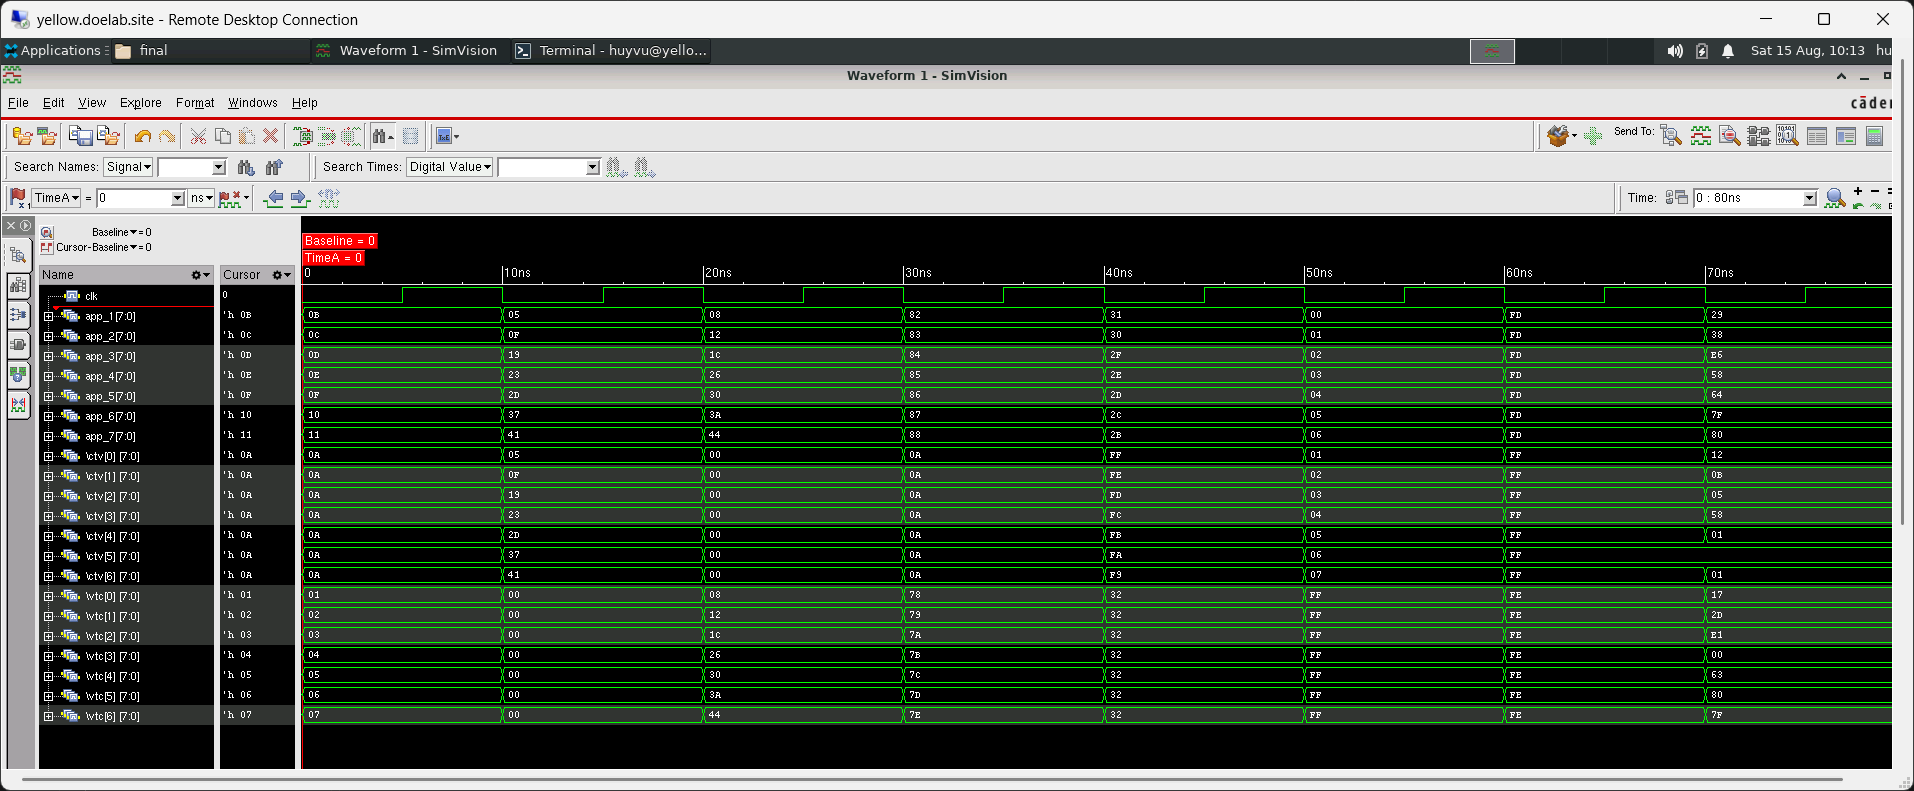
\includegraphics[width=\textwidth]{./images/ctv_app_calc_waveform.png}
    \caption{Dạng sóng của khối CTV APP Calculation}
\end{figure}


\begin{itemize}
    \item Giai đoạn cộng số nguyên cơ bản (0 ns - 10 ns): Tín hiệu ctv duy trì hằng số 8'h0A (10 thập phân) trên cả 7 kênh, còn vtc tăng dần từ 8'h01 đến 8'h07. Bus ngõ ra app phản ánh tức thì giá trị tổng tương ứng từ 8'h0B đến 8'h11. Mạch đáp ứng chuẩn xác tính chất cộng tuyến tính $app_i = vtc_i + 10$.
    \item Giai đoạn kiểm tra phần tử trung tính (10 ns - 30 ns): Từ 10 ns - 20 ns, vtc bị kéo xuống 8'h00. Ngõ ra app sao chép hoàn toàn giá trị của ctv. Từ 20 ns - 30 ns, ctv bị kéo xuống 8'h00. Ngõ ra app sao chép hoàn toàn giá trị của vtc.Mạch xác nhận không có hiện tượng sai lệch dữ liệu hay gán nhầm mức logic khi một trong hai vector ngõ vào bằng $0$.
    \item Giai đoạn xử lý số âm bù 2 và hiện tượng tràn bit (40 ns - 60 ns): Tại 40 ns, ctv mang các giá trị từ 8'hFF giảm dần đến 8'hF9. Phép cộng với vtc = 8'h32 cho ra kết quả app giảm dần từ 8'h31 đến 8'h2B, thể hiện đúng bản chất phép trừ trong hệ thống Bù 2. Tại 50 ns, vtc đạt giá trị cực đại 8-bit 8'hFF. Khi cộng thêm 8'h01, kết quả $255 + 1 = 256$ bị tràn bit nhớ $Co$, phần dữ liệu 8-bit còn lại của app\_1 xoay vòng về 8'h00. Tương tự, app\_7 nhận $255 + 7 = 262 \Rightarrow 8'h06$.
\end{itemize}

\begin{table}[H]
\centering
\resizebox{0.8\textwidth}{!}{
\begin{tabular}{|l|c|c|}
\hline
\textbf{Library Name} 
& \textbf{Total Area} 
& \textbf{Total Power} \\
\hline

fast\_vdd1v0\_basicCells\_hvt & 404.586 & 3.68958e-04 \\ \hline
fast\_vdd1v2\_basicCells\_hvt & 404.586 & 5.34551e-04 \\ \hline
slow\_vdd1v0\_basicCells\_hvt & 821.826 & 3.34493e-04 \\ \hline
slow\_vdd1v2\_basicCells\_hvt & 569.772 & 4.02237e-04 \\ \hline
fast\_vdd1v0\_basicCells\_lvt & 404.586 & 3.80819e-04 \\ \hline
fast\_vdd1v2\_basicCells\_lvt & 275.310 & 5.38660e-04 \\ \hline
slow\_vdd1v0\_basicCells\_lvt & 483.588 & 2.77465e-04 \\ \hline
slow\_vdd1v2\_basicCells\_lvt & 483.588 & 3.97555e-04 \\ \hline

\end{tabular}
}
\caption{Tổng hợp thông số Diện tích và Công suất của khối Min/Submin Calculationn qua các process corners.}
\end{table}

\textbf{Phân tích Diện tích (Total Area):}
\begin{itemize}
    \item Tác động của góc PVT và sụt áp: Diện tích mạch đạt giá trị lớn nhất ở góc slow\_vdd1v0\_basicCells\_hvt (821.826). Ở điều kiện sụt áp (1.0V/0.9V) và nhiệt độ cao, độ trễ linh kiện tăng mạnh, buộc công cụ tổng hợp phải tăng kích thước cell và chèn thêm nhiều buffer/cổng logic phụ để thỏa mãn ràng buộc thời gian.
    \item Hiệu quả tối ưu diện tích của cell LVT: Ở góc Slow 1.0V, thư viện LVT giúp giảm diện tích xuống 483.588 (giảm 41.2\% so với HVT). Do dòng lái của LVT mạnh hơn ở điện áp thấp, công cụ tổng hợp không cần gia tăng kích thước cell quá lớn để đạt timing.
    \item Cực tiểu diện tích: Diện tích nhỏ nhất đạt được ở góc fast\_vdd1v2\_basicCells\_lvt (275.310), giảm 31.9\% so với mức tiêu chuẩn 404.586 (ở các góc Fast 1.0V). Điện áp cao (1.2V) kết hợp với $V_{th}$ thấp giúp các cổng logic kích thước tối thiểu vẫn đảm bảo tốc độ chuyển mạch.
\end{itemize}

\textbf{Phân tích Công suất tiêu thụ (Total Power):}
\begin{itemize}
    \item Sự phụ thuộc vào Điện áp cấp ($V_{dd}$): Điện áp là yếu tố chi phối chính tới tổng công suất tiêu thụ do thành phần công suất động tỉ lệ thuận với $V_{dd}^2$. Khi tăng điện áp từ 1.0V lên 1.2V: Trong thư viện HVT (góc Fast): Công suất tăng từ $3.68958 \times 10^{-4}$ lên $5.34551 \times 10^{-4}$ (tăng 44.9\%). Trong thư viện LVT (góc Fast): Công suất tăng từ $3.80819 \times 10^{-4}$ lên $5.38660 \times 10^{-4}$ (tăng 41.4\%).
    \item So sánh công suất HVT và LVT: Tại góc Fast (1.0V): Công suất của LVT ($3.80819 \times 10^{-4}$) cao hơn HVT ($3.68958 \times 10^{-4}$) do điện áp ngưỡng thấp làm tăng dòng rò (leakage power). Tại góc Slow (1.0V): Công suất của LVT ($2.77465 \times 10^{-4}$) lại thấp hơn HVT ($3.34493 \times 10^{-4}$). Nguyên nhân do thiết kế HVT ở góc này có diện tích tăng vọt (821.826 so với 483.588), làm tăng điện dung chuyển mạch tổng và kéo theo công suất động tăng cao.
    \item Công suất thấp nhất: Đạt $2.77465 \times 10^{-4}$ ở góc slow\_vdd1v0\_basicCells\_lvt nhờ giảm thiểu điện áp và quy mô diện tích gọn nhẹ. Công suất cao nhất: Đạt $5.38660 \times 10^{-4}$ ở góc fast\_vdd1v2\_basicCells\_lvt do hoạt động ở mức điện áp đỉnh (1.2V/1.32V) kết hợp tần số đóng cắt cao.
\end{itemize}

\begin{table}[h]
\centering
\resizebox{\textwidth}{!}{%
\begin{tabular}{@{}clp{8.5cm}cc@{}}
\toprule
\textbf{STT} & \textbf{Góc PVT} & \textbf{Đường đi tín hiệu (Critical Path)} & \textbf{Độ trễ (ps)} & \textbf{Thời gian dư (ps)} \\ \midrule
1 & fast\_1v0\_hvt & ctv\_7[0] $\rightarrow$ ADDHX2HVT $\rightarrow$ ADDFX2HVT ($\times 6$) $\rightarrow$ XNOR2X2HVT $\rightarrow$ app\_7[7] & 687 & 463 \\
2 & fast\_1v2\_hvt & ctv\_7[0] $\rightarrow$ ADDHX2HVT $\rightarrow$ ADDFX2HVT ($\times 6$) $\rightarrow$ XNOR2X2HVT $\rightarrow$ app\_7[7] & 488 & 662 \\
3 & slow\_1v0\_hvt & ctv\_7[0] $\rightarrow$ CLKAND2X6HVT $\rightarrow$ INVX4HVT $\rightarrow$ OAI21X4HVT $\rightarrow$ NAND2X2HVT ($\times 2$) $\rightarrow$ OAI2BB1X1HVT $\rightarrow$ NAND2X2HVT ($\times 2$) $\rightarrow$ OAI2BB1X1HVT $\rightarrow$ NAND2X1HVT ($\times 2$) $\rightarrow$ XNOR2X1HVT $\rightarrow$ BUFX16HVT $\rightarrow$ app\_7[7] & 1692 & -542 \\
4 & slow\_1v2\_hvt & ctv\_7[0] $\rightarrow$ INVX1HVT $\rightarrow$ NOR2BX1HVT $\rightarrow$ (OAI21X1HVT $\rightarrow$ OAI2BB1X1HVT) ($\times 6$) $\rightarrow$ CLKMX2X6HVT $\rightarrow$ app\_7[7] & 1029 & 121 \\
5 & fast\_1v0\_lvt & ctv\_7[0] $\rightarrow$ ADDHX2LVT $\rightarrow$ ADDFX2LVT ($\times 6$) $\rightarrow$ XNOR2X2LVT $\rightarrow$ app\_7[7] & 383 & 767 \\
6 & fast\_1v2\_lvt & vtc\_7[0] $\rightarrow$ ADDHX1LVT $\rightarrow$ ADDFX1LVT ($\times 6$) $\rightarrow$ XNOR2X1LVT $\rightarrow$ app\_7[7] & 336 & 814 \\
7 & slow\_1v0\_lvt & ctv\_7[0] $\rightarrow$ AND2XLLVT $\rightarrow$ ADDFX4LVT $\rightarrow$ OAI21X1LVT $\rightarrow$ OAI2BB1X1LVT $\rightarrow$ ADDFX4LVT ($\times 3$) $\rightarrow$ ADDHX4LVT $\rightarrow$ XNOR2X4LVT $\rightarrow$ app\_7[7] & 1122 & 28 \\
8 & slow\_1v2\_lvt & ctv\_7[0] $\rightarrow$ ADDHX1LVT $\rightarrow$ ADDFX4LVT ($\times 6$) $\rightarrow$ XNOR2X4LVT $\rightarrow$ app\_7[7] & 733 & 417 \\ \bottomrule
\end{tabular}%
}
\caption{Thống kê độ trễ các góc phân tích (PVT corners) cho khối ctv\_app\_calc.}
\end{table}

\begin{itemize}
    \item Tác động của Điện áp cấp ($V_{dd}$): Việc nâng điện áp hoạt động từ 1.0V lên 1.2V làm giảm đáng kể độ trễ đường truyền dữ liệu và tăng lượng thời gian dư trên mọi góc PVT. Ví dụ ở điều kiện Fast HVT, thời gian trễ giảm từ 687 ps xuống 488 ps (Slack tăng từ 463 ps lên 662 ps).
    \item So sánh hiệu năng HVT và LVT: Thư viện LVT ($V_{th}$ thấp) cho tốc độ đáp ứng chuyển mạch vượt trội so với HVT. Tại góc fast\_1v0, LVT giảm trễ tới 44.2\% so với HVT (383 ps so với 687 ps). Đặc biệt ở điều kiện Slow 1.0V, LVT vẫn thỏa mãn thời gian đáp ứng (Slack = 28 ps), trong khi HVT không đáp ứng được yêu cầu (Slack = -542 ps).
    \item Góc tới hạn: Góc slow\_1v0\_hvt là trường hợp xấu nhất gây vi phạm thời gian nghiêm trọng (Slack âm -542 ps, Data Path kéo dài đến 1692 ps). Ở điều kiện nhiệt độ cao (125°C) và điện áp thấp, công cụ tổng hợp bị chèn chuỗi phức tạp các cổng logic nhỏ (CLKAND2, NAND2, OAI2BB1, BUFX16) làm tăng số tầng logic (logic depth).
\end{itemize}


% %%%%%%%%%%%%%%%%%%%%

% \chapter{Kết quả thực hiện}
% Present the results of your implementation. Discuss:
% \begin{itemize}
%     \item The performance metrics and evaluation criteria.
%     \item Results obtained from testing and validation.
%     \item Comparisons with existing solutions or benchmarks.
%     \item Analysis and interpretation of results.
%     \item Any unexpected findings or observations.
% \end{itemize}

% %%%%%%%%%%%%%%%%%%%%

\chapter{Kết luận và hướng phát triển}
\section{Kết luận}
Trong quá trình thực hiện đề tài, em đã nghiên cứu các kiến thức cơ bản về mã LDPC, mã QC-LDPC và nguyên lý của thuật toán giải mã Min-Sum, từ đó phân tích các yêu cầu cần thiết để hiện thực thuật toán trên phần cứng FPGA. Trên cơ sở đó, kiến trúc bộ giải mã được phân tích và phân chia thành các khối chức năng phù hợp với đặc điểm xử lý song song và yêu cầu lưu trữ dữ liệu của thuật toán.

Về mặt thiết kế, em đã hoàn thành việc xây dựng các khối phần cứng cần thiết cho kiến trúc bộ giải mã bằng SystemVerilog. Việc phân chia thiết kế thành các khối chức năng độc lập cũng giúp thuận lợi cho quá trình kiểm tra, mô phỏng và tổng hợp. Kết quả mô phỏng RTL cho thấy các chức năng chính của thiết kế hoạt động đúng theo nguyên lý thuật toán đã phân tích. Các quá trình lưu trữ, truyền và xử lý dữ liệu trong kiến trúc được kiểm tra thông qua các trường hợp mô phỏng khác nhau, qua đó bước đầu xác nhận tính đúng đắn về mặt chức năng của thiết kế. Bên cạnh kiểm tra chức năng, em cũng đã thực hiện quá trình tổng hợp và đánh giá thiết kế tại nhiều điều kiện PVT khác nhau. Các thông số như diện tích phần cứng, độ trễ đường truyền và timing slack đã được khảo sát nhằm đánh giá khả năng đáp ứng của kiến trúc trong những điều kiện hoạt động khác nhau. Kết quả cho thấy điện áp nguồn, nhiệt độ và loại thư viện cell có ảnh hưởng đáng kể đến đặc tính timing của thiết kế. Đặc biệt, các điều kiện điện áp thấp và nhiệt độ cao tạo ra những trường hợp bất lợi hơn về mặt thời gian, trong khi việc sử dụng thư viện LVT có thể cải thiện đáng kể tốc độ hoạt động.

Tuy nhiên, do thời gian thực hiện đề tài còn hạn chế và tiến độ thực hiện tương đối gấp rút, kết quả hiện tại vẫn còn một số điểm chưa hoàn thiện. Thiết kế mới chủ yếu được kiểm chứng thông qua mô phỏng RTL và quá trình tổng hợp, chưa được triển khai hoàn chỉnh lên FPGA kit thực tế. Vì vậy, các kết quả về khả năng hoạt động trong môi trường phần cứng thực, tốc độ xử lý thực tế, mức sử dụng tài nguyên FPGA và công suất tiêu thụ thực tế vẫn chưa được kiểm chứng đầy đủ. Bên cạnh đó, một số kết quả phân tích timing tại các góc PVT bất lợi vẫn còn tồn tại vi phạm timing. Điều này cho thấy thiết kế vẫn cần được tiếp tục tối ưu về độ sâu logic, cấu trúc xử lý song song và đường truyền dữ liệu trước khi có thể đạt được hiệu năng mục tiêu trong mọi điều kiện hoạt động. Ví dụ, kết quả phân tích cho thấy tại điều kiện slow, điện áp thấp và nhiệt độ cao, một số đường dữ liệu có thể xuất hiện slack âm và trở thành các đường tới hạn của thiết kế.

Nhìn chung, mặc dù chưa thể hoàn thiện toàn bộ các bước của một quy trình triển khai phần cứng hoàn chỉnh, đề tài đã đạt được các mục tiêu chính trong phạm vi thời gian cho phép, đồng thời giúp em có thêm kinh nghiệm thực tế trong việc nghiên cứu thuật toán, thiết kế phần cứng số, mô phỏng RTL và sử dụng các công cụ EDA phục vụ cho quá trình tổng hợp và đánh giá thiết kế.

\section{Định hướng phát triển}

Trong thời gian tới, hướng phát triển đầu tiên của đề tài là tiếp tục hoàn thiện việc tích hợp các thành phần đã thiết kế thành một hệ thống giải mã QC-LDPC hoàn chỉnh ở mức top-level. Khi đó, toàn bộ luồng dữ liệu từ đầu vào, quá trình giải mã lặp cho đến dữ liệu đầu ra sẽ được kiểm tra thống nhất thay vì chỉ đánh giá từng thành phần ở mức riêng lẻ.

Một hướng phát triển quan trọng là triển khai thiết kế lên FPGA kit thực tế. Đây là bước cần thiết để kiểm chứng khả năng hoạt động của kiến trúc trong môi trường phần cứng thực tế. Sau khi triển khai, có thể tiến hành đo đạc tần số hoạt động, throughput, latency, mức sử dụng tài nguyên và công suất tiêu thụ, từ đó đánh giá chính xác hơn hiệu quả của kiến trúc so với các kết quả thu được từ mô phỏng và tổng hợp.

Bên cạnh đó, thiết kế cần tiếp tục được tối ưu về timing nhằm loại bỏ các đường truyền còn vi phạm tại những góc PVT bất lợi. Có thể nghiên cứu các phương pháp như giảm độ sâu logic, tối ưu cấu trúc tính toán, cân bằng đường truyền hoặc áp dụng pipeline ở những vị trí phù hợp. Mục tiêu là nâng cao tần số hoạt động nhưng vẫn duy trì diện tích và công suất ở mức hợp lý.

Về mặt kiến trúc, có thể tiếp tục nghiên cứu phương pháp tổ chức bộ nhớ và mức độ song song của quá trình xử lý nhằm tăng băng thông dữ liệu và throughput của bộ giải mã. Đồng thời, thiết kế có thể được mở rộng theo hướng tham số hóa để hỗ trợ nhiều cấu hình QC-LDPC khác nhau, giúp tăng tính linh hoạt và khả năng ứng dụng của kiến trúc.

Như vậy, kết quả đạt được trong đề tài có thể xem là bước nền tảng cho quá trình phát triển một kiến trúc giải mã QC-LDPC hoàn chỉnh trên FPGA. Mặc dù vẫn còn những hạn chế do thời gian thực hiện và chưa triển khai trên kit thực tế, các kết quả về thiết kế, mô phỏng và đánh giá phần cứng đã tạo tiền đề để tiếp tục tối ưu và hoàn thiện hệ thống trong các giai đoạn nghiên cứu tiếp theo.

%%%%%%%%%%References part%%%%%%%%%%%%%%%%%%%%%

\printbibliography[title=Tài liệu tham khảo]

Mã nguồn toàn bộ chương trình: \href{https://github.com/Jacksurfer2005/SummerInternshipPorject/tree/main/code}{Link} 
\end{document}